\def\year{2021}\relax
%File: formatting-instructions-latex-2021.tex
%release 2021.2
\documentclass[letterpaper]{article} % DO NOT CHANGE THIS
\usepackage{aaai21}  % DO NOT CHANGE THIS
\usepackage{times}  % DO NOT CHANGE THIS
\usepackage{helvet} % DO NOT CHANGE THIS
\usepackage{courier}  % DO NOT CHANGE THIS
\usepackage[hyphens]{url}  % DO NOT CHANGE THIS
\usepackage{graphicx} % DO NOT CHANGE THIS
\urlstyle{rm} % DO NOT CHANGE THIS
\def\UrlFont{\rm}  % DO NOT CHANGE THIS
\usepackage{natbib}  % DO NOT CHANGE THIS AND DO NOT ADD ANY OPTIONS TO IT
\usepackage{caption} % DO NOT CHANGE THIS AND DO NOT ADD ANY OPTIONS TO IT
\frenchspacing  % DO NOT CHANGE THIS
\setlength{\pdfpagewidth}{8.5in}  % DO NOT CHANGE THIS
\setlength{\pdfpageheight}{11in}  % DO NOT CHANGE THIS
%\nocopyright
%PDF Info Is REQUIRED.
% For /Author, add all authors within the parentheses, separated by commas. No accents or commands.
% For /Title, add Title in Mixed Case. No accents or commands. Retain the parentheses.
\pdfinfo{
/Title (AAAI Press Formatting Instructions for Authors Using LaTeX -- A Guide)
/Author (AAAI Press Staff, Pater Patel Schneider, Sunil Issar, J. Scott Penberthy, George Ferguson, Hans Guesgen, Francisco Cruz, Marc Pujol-Gonzalez)
/TemplateVersion (2021.2)
} %Leave this
% /Title (Conversational Neuro-Symbolic Commonsense Reasoning)
% Put your actual complete title (no codes, scripts, shortcuts, or LaTeX commands) within the parentheses in mixed case
% Leave the space between \Title and the beginning parenthesis alone
% /Author (Forough Arabshahi, Jennifer Lee, Mikayla Gawarecki, Kathryn Mazaitis, Amos Azaria, Tom Mitchell)
% Put your actual complete list of authors (no codes, scripts, shortcuts, or LaTeX commands) within the parentheses in mixed case.
% Each author should be only by a comma. If the name contains accents, remove them. If there are any LaTeX commands,
% remove them.

% DISALLOWED PACKAGES
% \usepackage{authblk} -- This package is specifically forbidden
% \usepackage{balance} -- This package is specifically forbidden
% \usepackage{color (if used in text)
% \usepackage{CJK} -- This package is specifically forbidden
% \usepackage{float} -- This package is specifically forbidden
% \usepackage{flushend} -- This package is specifically forbidden
% \usepackage{fontenc} -- This package is specifically forbidden
% \usepackage{fullpage} -- This package is specifically forbidden
% \usepackage{geometry} -- This package is specifically forbidden
% \usepackage{grffile} -- This package is specifically forbidden
% \usepackage{hyperref} -- This package is specifically forbidden
% \usepackage{navigator} -- This package is specifically forbidden
% (or any other package that embeds links such as navigator or hyperref)
% \indentfirst} -- This package is specifically forbidden
% \layout} -- This package is specifically forbidden
% \multicol} -- This package is specifically forbidden
% \nameref} -- This package is specifically forbidden
% \usepackage{savetrees} -- This package is specifically forbidden
% \usepackage{setspace} -- This package is specifically forbidden
% \usepackage{stfloats} -- This package is specifically forbidden
% \usepackage{tabu} -- This package is specifically forbidden
% \usepackage{titlesec} -- This package is specifically forbidden
% \usepackage{tocbibind} -- This package is specifically forbidden
% \usepackage{ulem} -- This package is specifically forbidden
% \usepackage{wrapfig} -- This package is specifically forbidden
% DISALLOWED COMMANDS
% \nocopyright -- Your paper will not be published if you use this command
% \addtolength -- This command may not be used
% \balance -- This command may not be used
% \baselinestretch -- Your paper will not be published if you use this command
% \clearpage -- No page breaks of any kind may be used for the final version of your paper
% \columnsep -- This command may not be used
% \newpage -- No page breaks of any kind may be used for the final version of your paper
% \pagebreak -- No page breaks of any kind may be used for the final version of your paperr
% \pagestyle -- This command may not be used
% \tiny -- This is not an acceptable font size.
% \vspace{- -- No negative value may be used in proximity of a caption, figure, table, section, subsection, subsubsection, or reference
% \vskip{- -- No negative value may be used to alter spacing above or below a caption, figure, table, section, subsection, subsubsection, or reference

\setcounter{secnumdepth}{2} %May be changed to 1 or 2 if section numbers are desired.

% The file aaai21.sty is the style file for AAAI Press
% proceedings, working notes, and technical reports.
%

% Title

% Your title must be in mixed case, not sentence case.
% That means all verbs (including short verbs like be, is, using,and go),
% nouns, adverbs, adjectives should be capitalized, including both words in hyphenated terms, while
% articles, conjunctions, and prepositions are lower case unless they
% directly follow a colon or long dash

\title{Conversational Neuro-Symbolic Commonsense Reasoning}

% \author{submission 8179}

\author{Forough Arabshahi\textsuperscript{\rm 1}\footnote{work done when FA and JL were at Carnegie Mellon University.}, Jennifer Lee\textsuperscript{\rm 1}, Mikayla Gawarecki\textsuperscript{\rm 2}\\ Kathryn Mazaitis\textsuperscript{\rm 2}, Amos Azaria\textsuperscript{\rm 3}, Tom Mitchell\textsuperscript{\rm 2}\\ % All authors must be in the same font size and format. Use \Large and \textbf to achieve this result when breaking a line
}

\affiliations{
\textsuperscript{\rm 1}Facebook,
\textsuperscript{\rm 2}Carnegie Mellon University, \textsuperscript{\rm 3}Ariel University\\
\{forough, jenniferlee98\}@fb.com, \{mgawarec, krivard\}@cs.cmu.edu,\\ amos.azaria@ariel.ac.il, tom.mitchell@cs.cmu.edu} 
 

% \title{AAAI Press Formatting Instructions \\for Authors Using \LaTeX{} --- A Guide }
% \author{
%     %Authors
%     % All authors must be in the same font size and format.
%     Written by AAAI Press Staff\textsuperscript{\rm 1}\thanks{With help from the AAAI Publications Committee.}\\
%     AAAI Style Contributions by Pater Patel Schneider,
%     Sunil Issar,  \\
%     J. Scott Penberthy,
%     George Ferguson,
%     Hans Guesgen,
%     Francisco Cruz,
%     Marc Pujol-Gonzalez
%     \\
% }
% \affiliations{
%     %Afiliations
%     \textsuperscript{\rm 1}Association for the Advancement of Artificial Intelligence\\
%     %If you have multiple authors and multiple affiliations
%     % use superscripts in text and roman font to identify them.
%     %For example,

%     % Sunil Issar, \textsuperscript{\rm 2}
%     % J. Scott Penberthy, \textsuperscript{\rm 3}
%     % George Ferguson,\textsuperscript{\rm 4}
%     % Hans Guesgen, \textsuperscript{\rm 5}.
%     % Note that the comma should be placed BEFORE the superscript for optimum readability

%     2275 East Bayshore Road, Suite 160\\
%     Palo Alto, California 94303\\
%     % email address must be in roman text type, not monospace or sans serif
%     publications21@aaai.org

%     % See more examples next
% }
% \iffalse
% %Example, Single Author, ->> remove \iffalse,\fi and place them surrounding AAAI title to use it
% \title{My Publication Title --- Single Author}
% \author {
%     % Author
%     Author Name \\
% }

% \affiliations{
%     Affiliation \\
%     Affiliation Line 2 \\
%     name@example.com
% }
% \fi

% \iffalse
% %Example, Multiple Authors, ->> remove \iffalse,\fi and place them surrounding AAAI title to use it
% \title{My Publication Title --- Multiple Authors}
% \author {
%     % Authors
%     First Author Name,\textsuperscript{\rm 1}
%     Second Author Name, \textsuperscript{\rm 2}
%     Third Author Name \textsuperscript{\rm 1} \\
% }
% \affiliations {
%     % Affiliations
%     \textsuperscript{\rm 1} Affiliation 1 \\
%     \textsuperscript{\rm 2} Affiliation 2 \\
%     firstAuthor@affiliation1.com, secondAuthor@affilation2.com, thirdAuthor@affiliation1.com
% }
% \fi



 
%%%%%%%%%%%%%%%%%%%%%%%%%%%%%%%%%%%%%%%%%%%%%%%%%%%%%%%%
% Recommended, but optional, packages for figures and better typesetting:
\usepackage{microtype}
\usepackage{booktabs} % for professional tables
%%%%%%%%%%%%%%%%%%%%%%%%%%%%%%%%%%%%%%%%%%%%%%%%%%%%%%%%
\usepackage{soul}
\usepackage{epsf,psfrag,amssymb,amsfonts,latexsym,bm,xcolor,array}
\usepackage{subcaption}
\usepackage{caption}
\captionsetup[table]{skip=3pt}
\usepackage{verbatim}
\usepackage[mathscr]{eucal}
\usepackage[tbtags]{mathtools}
\usepackage{multirow}
\usepackage{amsmath}
\usepackage{enumitem}
\usepackage{thmtools,thm-restate}
% \usepackage{algorithmicx}
\usepackage{algorithm}
\usepackage{algpascal}
\usepackage{algc}
\usepackage{algcompatible}
\usepackage[noend]{algpseudocode}
\usepackage[utf8]{inputenc}
\usepackage[english]{babel}
% \usepackage{authblk}
%\usepackage{titling}
% \usepackage{wrapfig}
\usepackage{tabularx}
% \usepackage{subcaption}
% \usepackage{multicol}
\usepackage{url}
% \usepackage{natbib}
\usepackage{listings}
\usepackage{makecell}
% \usepackage{cite}
% \usepackage[cal=zapfc,calscaled=1.15,bb=fourier,bbscaled=.96]{mathalfa}
\usepackage{bbold}
% \usepackage{lineno}

% Addition by kmm for system diagram:
\usepackage{tikz}
\usetikzlibrary{
shapes,
shapes.geometric,
shapes.misc,
arrows.meta,
quotes,
graphs,
positioning}
% end diagram additions


% \newcommand{\citet}[1]{\citeauthor{#1}~\shortcite{#1}} 
% \newcommand{\citep}{\cite} \newcommand{\citealp}[1]{\citeauthor{#1}~\citeyear{#1}}
% \newcommand{\cite}[1]{\citeauthor{#1}~\shortcite{#1}} 
%%%%%%%%%%%%%%%%%%%%%%%%%%%%%%%%%%%%%%%%%%%%%%%%%%%%%%%%
% algorithm commands
\algnewcommand\algorithmicinput{\textbf{Input:}}
\algnewcommand\Input{\item[\algorithmicinput]}
\algnewcommand\algorithmicoutput{\textbf{Output:}}
\algnewcommand\Output{\item[\algorithmicoutput]}

%%%%%%%%%%%%%%%%%%%%%%%%%%%%%%%%%%%%%%%%%%%%%%%%%%%%%%%%
% colors

\definecolor{bondiblue}{rgb}{0.0, 0.58, 0.71}
\definecolor{antiquefuchsia}{rgb}{0.57, 0.36, 0.51}
\definecolor{orange}{rgb}{1,0.5,0}
\definecolor{brickred}{rgb}{0.8, 0.25, 0.33}
\definecolor{gray(x11gray)}{rgb}{0.75, 0.75, 0.75}
\definecolor{lavendergray}{rgb}{0.77, 0.76, 0.82}
\definecolor{lightgray}{rgb}{0.83, 0.83, 0.83}
\definecolor{snow}{rgb}{1.0, 0.98, 0.98}
\definecolor{splashedwhite}{rgb}{1.0, 0.99, 1.0}
\definecolor{timberwolf}{rgb}{0.86, 0.84, 0.82}
\definecolor{seashell}{rgb}{1.0, 0.96, 0.93}
\definecolor{whitesmoke}{rgb}{0.96, 0.96, 0.96}
\definecolor{platinum}{rgb}{0.9, 0.89, 0.89}
\definecolor{pearl}{rgb}{0.94, 0.92, 0.84}
\definecolor{palepink}{rgb}{0.98, 0.85, 0.87}
\definecolor{oldlace}{rgb}{0.99, 0.96, 0.9}
\definecolor{mistyrose}{rgb}{1.0, 0.89, 0.88}
\definecolor{magnolia}{rgb}{0.97, 0.96, 1.0}
\definecolor{lavenderblush}{rgb}{1.0, 0.94, 0.96}
\definecolor{atomictangerine}{rgb}{1.0, 0.6, 0.4}
\definecolor{babyblue}{rgb}{0.54, 0.81, 0.94}
\definecolor{celadon}{rgb}{0.67, 0.88, 0.69}
\definecolor{darkpastelpurple}{rgb}{0.59, 0.44, 0.84}
\definecolor{flamingopink}{rgb}{0.99, 0.56, 0.67}
\definecolor{bluebell}{rgb}{0.64, 0.64, 0.82}
\definecolor{lavenderblue}{rgb}{0.8, 0.8, 1.0}
\definecolor{amethyst}{rgb}{0.6, 0.4, 0.8}
\definecolor{ao(english)}{rgb}{0.0, 0.5, 0.0}
\definecolor{cadmiumorange}{rgb}{0.93, 0.53, 0.18}
\definecolor{darkorange}{rgb}{1.0, 0.55, 0.0}
\definecolor{flame}{rgb}{0.89, 0.35, 0.13}
\definecolor{internationalorange}{rgb}{1.0, 0.31, 0.0}
\definecolor{alizarin}{rgb}{0.82, 0.1, 0.26}
\definecolor{cadmiumred}{rgb}{0.89, 0.0, 0.13}
\sethlcolor{lavenderblush}
\definecolor{candyapplered}{rgb}{1.0, 0.03, 0.0}
\definecolor{carminered}{rgb}{1.0, 0.0, 0.22}
\definecolor{carminepink}{rgb}{0.92, 0.3, 0.26}
\definecolor{coralred}{rgb}{1.0, 0.25, 0.25}
%%%%%%%%%%%%%%%%%%%%%%%%%%%%%%%%%%%%%%%%%%%%%%%%%%%%%%%%

\newcommand{\facomment}[1]{\noindent{\textcolor{magenta}{\textbf{\#\#\# FA:} \textsf{#1} \#\#\#}}} % Forough
\newcommand{\tmcomment}[1]{\noindent{\textcolor{olive}{\textbf{\#\#\# TM:} \textsf{#1} \#\#\#}}} % Tom
% \newcommand{\comment}[1]{\noindent{\textcolor{olive}{\textbf{\#\#\# TM:} \textsf{#1} \#\#\#}}} % Tom
% \newcommand{\aacomment}[1]{\noindent{\textcolor{blue}{\textbf{\#\#\# AA:} \textsf{#1} \#\#\#}}}
\newcommand{\amoscomment}[1]{\noindent{\textcolor{blue}{\textbf{\#\#\# AA:} \textsf{#1} \#\#\#}}} %Amos: I wasn't sure if I was supposed to use the 'AA', so I created another one.
\newcommand{\kmcomment}[1]{\noindent{\textcolor{orange}{\textbf{\#\#\# KM:} \textsf{#1} \#\#\#}}}
\newcommand{\mgcomment}[1]{\noindent{\textcolor{brown}{\textbf{\#\#\# MG:} \textsf{#1} \#\#\#}}}

\newcommand{\textGoal}{{\fontfamily{lmtt}\selectfont goal\,}}
\newcommand{\textAction}{{\fontfamily{lmtt}\selectfont action\,}}
\newcommand{\textState}{{\fontfamily{lmtt}\selectfont state\,}}
\newcommand{\art}{\fontfamily{pzc}\selectfont ART}
\newcommand{\CORGI}{CORGI}


\newcommand{\goal}{G(Z)}
\newcommand{\action}{A(Y)}
\newcommand{\state}{S(X)}
\newcommand{\KB}{$\mathcal{K}$}
\newcommand{\blank}{\textcolor{red}{$(\,\cdot^{^{\!\!\mkern-2mu\downarrow}})$}}
\newcommand{\nodelabel}[1]{\textcolor{red}{#1}}

\newcommand{\prologTerm}[1]{{\fontfamily{lmss}\selectfont \hl{#1}}}

\newcommand{\orangeTemplate}[2][atomictangerine]{ {\sethlcolor{#1} \hl{#2}} }
\newcommand{\blueTemplate}[2][babyblue]{ {\sethlcolor{#1} \hl{#2}} }
\newcommand{\greenTemplate}[2][celadon]{ {\sethlcolor{#1} \hl{#2}} }
\newcommand{\pinkTemplate}[2][flamingopink]{ {\sethlcolor{#1} \hl{#2}} }
\newcommand{\purpleTemplate}[2][lavenderblue]{ {\sethlcolor{#1} \hl{#2}} }
\newcommand{\redTemplate}[2][coralred]{ {\sethlcolor{#1} \hl{#2}} }

\newcommand{\comet}{$\mathbb{COMET}$}

\newcommand{\largeGap}{\qquad \qquad \qquad \qquad \qquad \qquad \quad}
%%%%%%%%%%%%%%%%%%%%%%%%%%%%%%%%%%%%%%%%%%%%%%%%%%%%%%%%

\begin{document}
% \linenumbers
\maketitle

\begin{abstract}
%Prior works in image conditioned text generation rely on end-to-end training with annotated caption data, which is expensive and computationally intensive.

% chatgpt refined
% Large-scale pre-trained language models (e.g.,GPT) have shown remarkable conversational and reasoning capabilities across many domains. 
% Recent studies has demonstrated the potential of leveraging CLIP latents to extend the capabilities of large language models to vision language tasks(e.g. image captioning) with text-only training. 
% Despite promising results of previous works, there remains a lack of a comprehensive and unified explanation of the prior approaches used and how CLIP latents can be fully leveraged in these applications.

Image captioning aims at generating descriptive and meaningful textual descriptions of images, enabling a broad range of vision-language applications. Prior works have demonstrated that harnessing the power of Contrastive Image Language Pre-training (CLIP) offers a promising approach to achieving zero-shot captioning, eliminating the need for expensive caption annotations. However, the widely observed modality gap in the latent space of CLIP harms the performance of zero-shot captioning by breaking the alignment between paired image-text features. To address this issue, we conduct an analysis on the CLIP latent space which leads to two findings. Firstly, we observe that the CLIP's visual feature of image subregions can achieve closer proximity to the paired caption due to the inherent information loss in text descriptions. In addition, we show that the modality gap between a paired image-text can be empirically modeled as a zero-mean Gaussian distribution. Motivated by the findings, we propose a novel zero-shot image captioning framework with text-only training to reduce the modality gap. In particular, we introduce a subregion feature aggregation to leverage local region information, which produces a compact visual representation for matching text representation. Moreover, we incorporate a noise injection and CLIP reranking strategy to boost captioning performance. We also extend our framework to build a zero-shot VQA pipeline, demonstrating its generality. Through extensive experiments on common captioning and VQA datasets such as MSCOCO, Flickr30k and VQAV2, we show that our method achieves remarkable performance improvements. Code is available at https://github.com/Artanic30/MacCap.

\end{abstract}
\section{Introduction}
% \vspace{-1em}
Despite the remarkable success of artificial intelligence (AI) and machine learning in the last few decades, commonsense reasoning remains an unsolved problem at the heart of AI \cite{levesque2012winograd,davis2015commonsense,sakaguchi2019winogrande}. 
Common sense allows us humans to engage in conversations with one another and to convey our thoughts efficiently, without the need to specify much detail \cite{grice1975logic}. For example, if Alice asks Bob to ``wake her up early whenever it snows at night'' so that she can get to work on time, Alice assumes that Bob will wake her up only if it snows enough to cause traffic slowdowns, and only if it is a working day. Alice does not explicitly state these conditions since Bob makes such \emph{presumptions} without much effort thanks to his common sense.
%does not need to explicitly mention that it needs to snow enough to cause traffic slowdowns and that it needs to be a working day for Bob to wake her up early; Bob makes these presumptions without much effort thanks to his common sense. 
A study, in which we collected such {\bf if(state)-then(action)} commands
% (similar to the previous example)
from human subjects, revealed that humans often under-specify conditions in their statements; perhaps because they are used to speaking with other humans who possess the common sense needed to infer their more specific intent by making presumptions about their statement.
% relying on the presumptions that their fellow humans would make about the statements. 
% Computers are currently unable to make these presumptions, making it challenging for them to engage in natural sounding conversations with humans.

The inability to make these presumptions makes it challenging 
% is one of the main reasons why 
%Amos: you can save some space by replacing "is one of the main reasons why it" with "makes it challenging..."
% it is challenging 
for computers to engage in natural sounding conversations with humans. While conversational AI systems such as Siri, Alexa, and others are entering our daily lives, their conversations with us humans remains limited to a set of pre-programmed tasks.
% Now is the right time to address this problem since conversational agents such as Siri, Alexa, and others are entering our daily lives yet their conversations with us humans remains limited to a set of pre-programmed tasks. %Amos: also here you can save some space by replacing "now is the right time to address this problem since" with "While conversational..." and remove "but"
We propose that handling unseen tasks requires conversational agents to develop common sense. % conversational agents need to develop common sense to handle unseen commands. %If we want to have conversational agents that resemble intelligent conversational interactions, then our conversational agents should be able to understand and execute   %The reason is that our conversational agents currently do not have the technology to correctly understand and execute new out-of-domain commands. We propose that one of the main reasons for this lack of understanding is that conversational agents lack commonsense reasoning. 
% into our daily lives in the past few years makes addressing this problem a timely contribution. This is becoming a prominent problem for computers in the recent years since computers are increasing their conversational interactions with humans

% \tmcomment{this is the problem we focus on in this paper. In the next parag we can say the problem more precisedly (Tom's sentence in the doc)} 
% In an attempt to enable this, 
Therefore, we propose a new commonsense reasoning benchmark for conversational agents where the task is to
% relevant to
% We consider a specific type of common sense reasoning relevant to
% understanding the intent of
infer \emph{commonsense presumptions} in commands of the form ``If \textState~holds Then perform \textAction~Because I want to achieve \textGoal.'' The {\bf if-(state), then-(action)} clause arises when humans instruct new conditional tasks to conversational agents \cite{azaria2016instructable, labutov2018lia}. 
The reason for including the \textbf{because-(goal)} clause in the commands is that some presumptions are ambiguous without knowing the user's purpose, or goal. For instance, if Alice's goal in the previous example was to see snow for the first time, Bob would have presumed that even a snow flurry would be excuse enough to wake her up. Since humans frequently omit details when stating such commands, a computer possessing common sense
% our interest lies in how computers
should be able to infer the hidden \emph{presumptions}; that is, the additional unstated conditions on the If and/or Then portion of the command. Please refer to Tab.~\ref{tab:statement_stats} for some examples. %although the presumptions in the above example are more natural, other scenarios can also occur:
% \vspace{-0.4em}
% \begin{itemize}
%     \item[$\mathcal{A}$)] Whenever it snows at night, then wake me up early, because I want to get to work on time.
%     \vspace{-0.4em}
%     \item[$\mathcal{B}$)] Whenever it snows at night, then wake me up early, because I have never seen snow before.
% \end{itemize}
% \vspace{-0.3em}
% A computer possessing common sense should be able to presume that a snow flurry does not trigger scenario $\mathcal{A}$ but triggers scenario $\mathcal{B}$. 
% For the above example, although that interpretation is more natural it is possible to have another scenario.
%which specify the goal of each if-then statement.
% The following is an example of two of the statements in our data set.

% in scenario $\mathcal{A}$ the speaker does not want to wake up early on a weekend, whereas in scenario $\mathcal{B}$ the speaker wants to wake up early regardless of the day. 
% It should also be able to presume that 

%   The under-specified statements in our data set are annotated with the presumptions that humans would make to fill in the unspoken details (Tab.~\ref{tab:statement_stats}).

% We consider in particular
\begin{table*}[t]
% \begin{minipage}[t][1in][t]{0.2\textwidth}
    \caption{Statistics of \textbf{if-(state), then-(action), because-(goal)} commands collected from a pool of human subjects. The table shows four distinct types of \emph{because}-clauses we found, the count of commands of each type, examples of each and their corresponding commonsense presumption annotations. {\em Restricted domain} includes commands whose \textState is limited to checking email, calendar, maps, alarms, and weather. {\em Everyday domain} includes commands concerning more general day-to-day activities. Annotations are tuples of (index, presumption) where index shows the starting word index of where the missing presumption should be in the command, highlighted with a red arrow. Index starts at 0 and is calculated for the original command.
    % Each type is accompanied by an example statement.
    }
    \label{tab:statement_stats}
    \centering
    \resizebox{0.85\textwidth}{!}{%
    \begin{tabular}{|cccc|lc|c|}
    \toprule
    \textbf{Domain} & 
        \parbox[b]{3em}{\centering \textbf{\textit{if} clause}} & 
        \parbox[b]{3em}{\centering \textbf{\textit{then} clause}} & 
        \parbox[b]{3em}{\textbf{\textit{because} clause}} & \textbf{Example} &  \parbox[b]{15em}{\centering \textbf{\textit{Annotation:}\\ Commonsense Presumptions}} & \textbf{Count} \\
        \midrule 
                  %LIA-compatible &  &  &  & 83 \\
         Restricted domain & state & action & goal & \thead[l]{If it's going to rain in the afternoon \blank \\ then remind me to bring an umbrella \blank \\ because I want to remain dry} & \thead{(8, and I am outside) \\ (15, before I leave the house)}  & 76\\
         Restricted domain & state & action & anti-goal & \thead[l]{If I have an upcoming bill payment \blank \\ then remind me to pay it \blank \\ because I don’t want to pay a late fee} & \thead{(7, in the next few days) \\	(13, before the bill payment deadline)} & 3\\
         Restricted domain & state & action & modifier & \thead[l]{If my flight \blank~is from 2am to 4am \\ then book me a supershuttle \blank \\ because it will be difficult to find ubers.} & \thead{(3, take off time) \\ (13, for 2 hours before my flight take off time)} & 2\\
         Restricted domain & state & action & conjunction & \thead[l]{If I receive emails about sales on basketball shoes \blank \\ then let me know \blank \\ because I need them and I want to save money.} & \thead{(9, my size) \\ (13, there is a sale)} & 2\\
%         \cline{1-1} \cline{5-5}
%\hline
         SUM &\ & & & & & 83\\
         \midrule
        %  & & & & & \\%\hline
         %Open domain  &  &  &  & 77\\
         Everyday domain & state & action & goal & \thead[l]{If there is an upcoming election  \blank \\ then remind me to register \blank~and vote \blank \\ because I want my voice to be heard.} & \thead{(6, in the next few months) \\ (6, and I am eligible to vote) \\ (11, to vote), (13, in the election)} & 55\\
         Everyday domain & state & action & anti-goal & \thead[l]{If it's been two weeks since my last call with my mentee \\ and I don't have an upcoming appointment with her \blank \\ then remind me to send her an email \blank \\ because we forgot to schedule our next chat} & \thead{(21, in the next few days) \\ (29, to schedule our next appointment)} & 4\\
         Everyday domain & state & action & modifier & \thead[l]{If I have difficulty sleeping \blank \\ then play a lullaby \\ because it soothes me.} & (5, at night) & 12 \\
         Everyday domain & state & action & conjunction &  \thead[l]{If the power goes out \blank \\ then when it comes back on remind me to restart the house furnace \\ because it doesn't come back on by itself and I want to stay warm} & (5, in the Winter) & 6 \\
%                  \cline{1-1} \cline{5-5}
%\hline
          SUM &  &  &  &  &  & 77\\
          \bottomrule 
    \end{tabular}
    }
    % \vspace{-1em}
\end{table*}
% \end{minipage}
%  \facomment{put an arrow for where the text should go. add more info. the different types of the because-clauses we have found (then point to the text)}

% % NO ANNOTATION
% \begin{table}[t]
%     \centering
%     \resizebox{0.7\textwidth}{!}{%
%     \begin{tabular}{|cccc|l|c|}
%     \toprule
%     \textbf{Domain} & 
%         \parbox[b]{3em}{\centering \textbf{\textit{if} clause}} & 
%         \parbox[b]{3em}{\centering \textbf{\textit{then} clause}} & 
%         \parbox[b]{3em}{\textbf{\textit{because} clause}} & \textbf{Example} & \textbf{Size} \\
%         \midrule 
%                   %LIA-compatible &  &  &  & 83 \\
%          Restricted domain & state & action & goal & \thead[l]{If it's going to rain in the afternoon \\ then remind me to bring an umbrella \\ because I want to remain dry} & 76\\
%          Restricted domain & state & action & anti-goal & \thead[l]{If I have an upcoming bill payment \\ then remind me to pay it \\ because I don’t want to pay a late fee} & 3\\
%          Restricted domain & state & action & modifier & \thead[l]{If my flight is from 2am to 4am \\ then book me a supershuttle \\ because it will be difficult to find ubers.} & 2\\
%          Restricted domain & state & action & conjunction & \thead[l]{If I receive emails about sales on basketball shoes \\ then let me know \\ because I need them and I want to save money.} & 2\\
% %         \cline{1-1} \cline{5-5}
% %\hline
%          SUM &\ & & & & 83\\
%          \midrule
%         %  & & & & & \\%\hline
%          %Open domain  &  &  &  & 77\\
%          Everyday domain & state & action & goal & \thead[l]{If there is an upcoming election \\ then remind me to register and vote \\ because I want my voice to be heard.} & 55\\
%          Everyday domain & state & action & anti-goal & \thead[l]{If it's been two weeks since my last call with my mentee \\ and I don't have an upcoming appointment with her \\ then remind me to send her an email \\ because we forgot to schedule our next chat} & 4\\
%          Everyday domain & state & action & modifier & \thead[l]{If I have difficulty sleeping \\ then play a lullaby \\ because it soothes me.} & 12 \\
%          Everyday domain & state & action & conjunction &  \thead[l]{If the power goes out \\ then when it comes back on remind me to restart the house furnace \\ because it doesn't come back on by itself and I want to stay warm} & 6 \\
% %                  \cline{1-1} \cline{5-5}
% %\hline
%           SUM &  &  &  &  & 77\\
%           \bottomrule 
%     \end{tabular}
%     }
%     \caption{Statistics of if-then-because statements collected from a pool of human subjects. The table shows the different types of \emph{because}-clauses we have found, the size of each, examples of each type and their corresponding commonsense presumption annotations. Restricted domain includes statements whose \textState is limited to checking email, calendar, maps, alarms, and weather. Everyday domain are statement concerning day-to-day activities.}
%     \label{tab:statement_stats}
% \end{table}
% \vspace{-0.8em}
In this paper, in addition to the proposal of this novel task and the release of a new dataset to study it, we propose a novel initial approach that infers such missing presumptions, by
extracting %completing
a chain of reasoning that shows how the commanded \textAction will achieve the desired \textGoal when the \textState holds. Whenever any additional reasoning steps appear in this reasoning chain, 
% presumptions are required to complete this chain of reasoning, 
they are output by our system as assumed implicit presumptions associated with the command. For our reasoning method we propose a neuro-symbolic interactive, conversational approach, in which the computer combines its own commonsense knowledge with conversationally evoked knowledge provided by a human user. The reasoning chain is extracted using our neuro-symbolic theorem prover that learns sub-symbolic representations (embeddings) for logical statements, making it robust to variations of natural language encountered in a conversational interaction setting. 
%To the best of our knowledge, no work in the literature studies this aspect of commonsense reasoning.
% \tmcomment{we consider here one form of commonsense reasoning that is used to }

% We release the if-then statements collected in our study as a benchmark for evaluating machine common sense. 
% The goal of the because explanation is to help disambiguate the above two scenarios.
% intentions of the user? The data is annotated with the gold under-specifications. \tmcomment{say that the condition is under-specified and the annotations are gold annotations that indicate what the condition should be [intended conditions/implicit condition] -> define this early on and then use these}
% In contrast to our task design, almost all the commonsense reasoning benchmarks such as \cite{levesque2012winograd,sakaguchi2019winogrande,roemmele2011choice,mostafazadeh2017lsdsem} are designed in a multi-choice manner. It has been shown that some incorrect answers in these benchmarks could be ruled out due to biases that are easily detectable by language models \cite{trinh2018simple, sakaguchi2019winogrande} resulting in an over-estimation of machine commonsense. %Tab.~\ref{tab:statement_stats} shows examples of our data.
% The task that we propose has a more open domain and a harder structure \facomment{reword, why is this exactly?}

% using soft logical reasoning.
% \facomment{motivate why logic? Why not directly use natural language reasoning chains? e.g. why not do: \cite{clark2020transformers}}.
% Our neuro-symbolic reasoning system is
% We propose a neuro-symbolic commonsense reasoning framework that uncovers commonsense presumptions in a given statement. It has a soft logic theorem prover at its heart that extracts chains of reasoning given an input if-then-because statement. For example, given statement $\mathcal{A}$ it extracts the following reasoning chain: $(1)$ if it snows more than two inches, then there will be traffic, $(2)$ if there is traffic, then my commute time to work increases, $(3)$ if my commute time to work increases then I need to leave the house earlier to ensure I get to work on time. Using this reasoning chain, it presumes that the speaker probably needs to wake up early only when it snows more than two inches. % This reasoning chain fills in the underspecified details in the original statement. For example, the amount of snow needed to cause traffic slowdowns, which is not explicitly mentioned in the statement.

% The first challenge that our theorem prover addresses is dealing with variations of natural language. These variations result in different logical surface forms for semantically similar statements. For example, ``it is going to snow at night'' is semantically similar to ``the forecast is calling for snow tonight'' but these have very different logical representations. Our theorem prover learns sub-symbolic representations (embeddings) that reflect the similarity between such phrases.

% \tmcomment{make it clear that we are referring to conversation}
% and either query it or propose automated knowledge base completion methods for it.
% The second challenge in performing reasoning is that the computer needs to have access to commonsense knowledge about the world. Most of the literature on reasoning relies on extracting the largest possible snapshot of world knowledge. However, there is currently no technology that has the capacity to store and query the sum total of all human knowledge, making current knowledge bases incomplete. Mimicking a human's strategy of accumulating knowledge, we argue that it is necessary to equip reasoning engines with a conversational interaction strategy facilitating the extraction of just-in-time information needed for reasoning. The advent of conversational agents like Siri, Alexa and others into our daily lives has made leveraging conversational interactions, a realistic and plausible opportunity.
% \tmcomment{make it clear that we are conversing with the user and not crawling the web e.g.} 
% This is \tmcomment{remove} because there is currently no technology that has the capacity to store and query the sum total of all human knowledge.
\paragraph{Contributions}
This paper presents three main contributions. 1) We propose a benchmark task for commonsense reasoning in conversational agents and release a data set containing \textbf{if-(state), then-(action), because-(goal)} commands, annotated with commonsense presumptions.
% \tmcomment{gold under-specifications -> not clear}.
2) We present CORGI (COmmonsense ReasoninG by Instruction), a system that performs soft logical inference. CORGI uses our proposed neuro-symbolic theorem prover and applies it to extract a multi-hop reasoning chain that reveals commonsense presumptions. %full condition.
3) We equip CORGI with a conversational interaction mechanism that enables it to collect just-in-time commonsense knowledge from humans.
% when encountering missing background knowledge. 
Our user-study shows (a) the plausibility of relying on humans to evoke commonsense knowledge and (b) the effectiveness of our theorem prover, enabling us to extract reasoning chains for up to 45\% of the studied tasks\footnote{The code and data are available here: https://github.com/ForoughA/CORGI}.

% Commonsense reasoning refers to our ability of making sense of the world around us and reasoning about it in our everyday life. \hl{give an example}. The hardest problem in commonsense reasoning is that when we humans talk to one another, we make assumptions about each other's world knowledge and therefore, under-specify many terms knowing that the other party will understand it, and that if they don't they will just ask for more explanation. 

% For example, if a human tells another human ``'' Many of the failures of AI systems today can be tracked back to the lack of commonsense \cite{}. For example, \hl{give some examples}. Therefore, it is becoming more and more important to develop machine learning algorithms that are capable of doing commonsense reasoning and take care of some of the problems that is so obvious to us humans todate. \facomment{bad wording need to rephrase everything}

% We argue in this paper, that one way of approaching commonsense is developing reasoning systems that are capable of extracting multi-hop chains of inference, similar to how humans logically think in their every day lives when they encounter ``trivial to us but hard for computers'' scenarios. we could cite \cite{battaglia2018relational} here.

% A trivial method for this is to represent knowledge in terms of first order logic (FOL) and then do logical inference to extract these reasoning chains. Logic inference systems are powerful and were designed and optimized for this task, but one major drawback of logical inference is that it is hard to generalize to unseen logic statements. In order to deal with this flaw, we propose a neuro-symbolic logical inference algorithm that learns sub-symbolic representations for logic statements.

% Neuro-symbolic models have recently gained widespread attention \cite{lamb2020graph,rocktaschel2017end,evans2018learning,arabshahi2018combining}. The symbolic aspect of these models provide structure while their neural aspect provide flexibility and these models use the best of both worlds allowing them to generalize to unseen problems in a systematic way \cite{battaglia2018relational, lake2017generalization, arabshahi2018combining, allamanis2017learning} These models bring in a symbolic flavor to conventional neural networks. The result is that these models leverage the power of symbolic computing, which is a major research focus ever since the formation of artificial intelligence, and overcome its main challenge which is dealing with noise and uncertainty. In this paper, we propose a neuro-symbolic automated theorem prover for the problem of commonsense reasoning.

% Commonsense reasoning is a challenging open problem in Artificial Intelligence. Despite the efforts of researchers \cite{levesque2012winograd,bosselut2019comet,sakaguchi2019winogrande}, computers are still far from perfect when it comes to commonsense. We study commonsense reasoning in the context of natural language if-then statements. For example, ``If it snows at night then wake me up 30 minutes earlier''. If a human encounters this statement, they will probably think ``this person is likely concerned about the fact that if it snows a lot, then there will be traffic and that if there is traffic they will need to wake up earlier to account for traffic and get to work on time''. In this paper, we study the possibility of the computer extracting the same thought process as a human by reducing commonsense reasoning to first order logical inference. The result of this is a multi-hop reasoning chain that resembles a human's thought process when making sense of the encountered statement. 

% The first challenge is performing such a reduction is the fact that natural language is highly noisy and ambiguous. Specifically, semantically similar natural language statements could have completely different structures and surface forms making FOL inference fail at solving this task. Therefore, we propose a neuro-symbolic inference algorithm that learns embeddings for logical statements that allows the system to overcome this challenge.



% We collected a data set of if-then statements from humans that we release with this paper and can be used as a benchmark for evaluating commonsense reasoning abilities. An interesting insight we have added when we collect these statements was to ask humans for the reason they want to perform an if-then task. In order to show why this is important consider the following two statements: ``If it snows tonight then wake me up early because I don't want to be late to work.'', v.s. ``If it snows tonight then wake me up early because I have never seen snow before.'' Comparing these two statements reveals the very different implications of each resulting is very different reasoning chains. To make it concrete, statements have a general format of ``if state $S$ occurs then do action $A$ because I want to achieve goal $G$'' and commonsense reasoning is the task of identifying how performing action $A$ in state $S$ allows one to achieve goal $G$. We would like to note that these are free-form natural language spoken text, and there is no specific template according to which these were collected other than being tied to the state/action/goal structure.


% \vspace{-1em}
\subsection{Related Work} %Amos: I guess there is no room for a section? I find paragraph a little odd, since there are multiple paragraphs here.
% Commonsense reasoning has been studied since the birth of AI 
The literature on commonsense reasoning dates back to the very beginning of the field of AI
\cite{winograd1972understanding,mueller2014commonsense,davis2015commonsense} and is studied in several contexts. 
One aspect focuses on building a large knowledge base (KB) of commonsense facts. %Examples are p
Projects like CYC \cite{lenat1990cyc}, ConceptNet \cite{liu2004conceptnet,havasi2007conceptnet, speer2017conceptnet} and ATOMIC \cite{sap2018atomic,rashkin2018event2mind} are examples of such KBs (see \cite{davis2015commonsense} for a comprehensive list). Recently, \citet{bosselut2019comet} proposed \comet{}, a neural knowledge graph that generates knowledge tuples by learning on examples of structured knowledge.
% trained on ConceptNet and ATOMIC, that generates commonsense facts. 
These KBs provide background knowledge for tasks that require common sense. % are developed to be used in other systems whose down stream task requires common sense. %Amos: does "this research effort" refer to \cite{bosselut2019comet} or to our paper? Forough: it refers to all the works in this paragraph
% Although it is important to have access to large knowledge bases in reasoning,
However, it is known that knowledge bases are incomplete, and most have ambiguities and inconsistencies \cite{davis2015commonsense} that must be clarified
% on the spot when being used 
for particular reasoning tasks. %Amos: I don't like the expression "on the spot" maybe "at the moment of"? Forough: is it better?
Therefore, we argue that 
% even with access to a knowledge base, 
reasoning engines can benefit greatly from a \emph{conversational interaction strategy} to ask humans about their missing or inconsistent knowledge. 
% We show here that it is reasonable to rely on humans for knowledge extraction. 
Closest in nature to this proposal is the work by \citet{hixon2015learning} on relation extraction through conversation for question answering and \citet{wu2018learning}'s system that learns to form simple concepts through interactive dialogue with a user. 
% \facomment{not sure if we should keep the following}
The advent of intelligent agents and advancements in natural language processing have given learning from conversational interactions a good momentum in the last few years
% Due to advances in natural language processing and the development of recent intelligent assistants, learning through conversational interactions has gained momentum in the past few years 
\citep{azaria2016instructable,labutov2018lia,srivastava2018teaching,goldwasser2014learning,christmann2019look,guo2018dialog,li2018appinite,li2017programming,li2017sugilite}.
% \cite{srivastava2017parsing,srivastava2017joint,}.
%Another counterpart of this type of learning is teaching by demonstration \citep{li2018appinite,li2017programming,li2017sugilite}. The reinforcement learning community has also seen recent interest in using natural language statements as instruction \citep{hu2019hierarchical,luketina2019survey,wang2016learning}.

A current challenge in commonsense reasoning is lack of benchmarks \cite{davis2015commonsense}. Benchmark tasks in commonsense reasoning include the Winograd Schema Challenge (WSC) \cite{levesque2012winograd}, its variations \cite{kocijan2020review}, and its recently scaled up counterpart, Winogrande \cite{sakaguchi2019winogrande} 
% (see \cite{kocijan2020review} for a comprehensive list of all variants of the WSC)
; ROCStories \cite{mostafazadeh2017lsdsem}, COPA \cite{roemmele2011choice}, Triangle COPA \cite{maslan2015one}, and {\art} \cite{bhagavatula2019abductive}, where the task is to choose a plausible outcome, cause or explanation for an input scenario; and the TimeTravel benchmark \cite{qin2019counterfactual} where the task to revise a story to make
it compatible with a given counterfactual
event. 
% in which given a story and two possible endings, the computer should indicate a plausible ending; and COPA \cite{roemmele2011choice} in which the computer should correctly choose the plausible cause of a given premise among two alternatives. Recently, \cite{bhagavatula2019abductive} released a challenge data set for abductive commonsense reasoning. 
Other than TimeTravel, most of these benchmarks have a multiple choice design format. 
% and it has been shown that some are prone to biases easily detectable by language models \cite{sakaguchi2019winogrande}. 
However, in the real world the computer is usually not given multiple choice questions.
% \tmcomment{if need to save space, delete next sentence.} Moreover, some incorrect answers in these benchmarks could be ruled out due to biases easily detectable by language models \cite{trinh2018simple, sakaguchi2019winogrande} resulting in an over-estimation of machine commonsense. 
None of these benchmarks targets the extraction of unspoken details in a natural language statement, which is a challenging task for computers known since the 1970's \cite{grice1975logic}. Note than inferring commonsense presumptions is different from intent understanding \cite{janivcek2010abductive,tur2011spoken} where the goal is to understand the intent of a speaker when they say, e.g., ``pick up the mug''. It is also different from implicature and presupposition \cite{sbisa1999presupposition,simons2013conversational,sakama2016abduction} which are concerned with what can be presupposed or implicated by a text.
% save space: Our proposed task has a more realistic design and is more challenging for computers. %\tmcomment{add that this benchmark is more realistic}
% Therefore, we propose a new benchmark for commonsense reasoning: extracting hidden commonsense presumptions given a natural language statement. 
% Commonsense reasoning has also been studied in textual and visual QA \cite{saeidi2018interpretation, yi2018neural,wu2018chain,zellers2019recognition,hudson2018compositional,narasimhan2018out,johnson2017inferring}, but an in depth review of these falls out of the scope of this work.

% We propose a neuro-symbolic solution (CORGI) that uncovers hidden presumptions in a given natural language statement using an extracted multi-hop reasoning chain. 
CORGI has a neuro-symbolic logic theorem prover. Neuro-symbolic systems are hybrid models that leverage the robustness of connectionist methods and the soundness of symbolic reasoning to effectively integrate learning and reasoning \cite{garcez2015neural,besold2017neural}. They have shown promise in different areas of logical reasoning ranging from classical logic to propositional logic, probabilistic logic, abductive logic, and inductive logic \cite{mao2019neuro, manhaeve2018deepproblog,dong2019neural,marra2019integrating,zhou2019abductive,evans2018learning}. To the best of our knowledge, neuro-symbolic solutions for commonsense reasoning have not been proposed before. Examples of commonsense reasoning engines are: AnalogySpace \cite{speer2008analogyspace,havasi2009digital} that uses dimensionality reduction
% such as PCA
and \citet{mueller2014commonsense} that uses the event calculus formal language. 
% Recently, \cite{wang2019satnet} proposed a differentiable maximum satisfiability solver for learning logical structures from data. The goal of works such as \cite{tran2016deep,hu2016harnessing}, which use logical rules in deep learning, is to improve the interpretability or performance of neural networks and are of less relevance here.
% In another line of research, logical rules have been used in deep learning to improve the interpretability or performance of neural networks \cite{tran2016deep,hu2016harnessing}. The goal of these works is not to directly address reasoning problems and is rather to improve the performance of neural networks by constraining their learning using a set of logical rules 
% essentially jointly learning using examples and rules 
% and is of less relevance to our work. %Although more recently \cite{wang2019satnet} proposed a maxSAT solver
% CORGI finds a chain of reasoning in a given commonsense knowledge base containing FOL facts and rules.
% Multi-hop reasoning is more challenging and indicates a higher capacity in performing reasoning
% Multi-hop reasoning for question answering has recently been explored and challenging benchmark data sets have been created in the community for it \citep{weston2015towards,welbl2018constructing,johnson2017clevr}. %\kmcomment{capacity for what? 'reasoning' is a bit circular}
% Chain of reasoning can be performed through logical inference and there are several interesting works that attempt to bridge the gap between symbolic reasoning and the recent advances in AI and machine learning \cite{liang2018symbolic,wang2019satnet}. %\cite{besold2017neural,}
% Another method that performs reasoning through logical inference is
TensorLog \citep{cohen2016tensorlog} converts a first-order logical database into a factor graph and proposes a differentiable strategy for belief propagation over the graph. DeepProbLog \cite{manhaeve2018deepproblog} developed a probabilistic logic programming language 
% and introduces the concept of a neural predicate. DeepProbLog 
that is suitable for applications containing categorical variables. %Amos: I think that the remainder of this section can be better organized.
Contrary to our approach, both these methods do not learn embeddings for logical rules that are needed
to make CORGI robust to natural language variations. 
Therefore, we propose an end-to-end differentiable solution that uses a Prolog \cite{colmerauer1990introduction} proof trace to learn rule embeddings from data. Our proposal is closest to the neural programmer interpreter \citep{reed2015neural} that uses the trace of algorithms such as addition and sort to learn their execution. 
The use of Prolog for performing multi-hop logical reasoning has been studied in \citet{rocktaschel2017end} and \citet{weber2019nlprolog}.
% where neural networks are integrated into Prolog to perform soft unification in backward chaining. 
% In these works, the authors propose differentiable ``AND'' and ``OR'' operations that convert unification to a differentiable process. 
These methods perform Inductive Logic Programming to learn rules from data, and are not applicable to our problem. 
% In order to address the scalability issues of \cite{rocktaschel2017end}, NLprolog \cite{weber2019nlprolog} proposes a non end-to-end differentiable solution. 
% a program \tmcomment{what program are they using?} to learn program execution.
DeepLogic \cite{cingillioglu2018deeplogic}, \citet{rocktaschel2014low}, and  \citet{wang2016blearning} also learn representations for logical rules using neural networks. 
% Other examples of works that learn low-dimensional embeddings for logic are 
%are %is [kmm- rephrase]
% \citep{rocktaschel2014low,wang2016blearning}. 
% \facomment{also cite: \cite{manhaeve2018deepproblog}}
Very recently, transformers were used for temporal logic \cite{finkbeiner2020teaching} and to do multi-hop reasoning \cite{clark2020transformers} using logical facts and rules stated in natural language. 
% Although the results are interesting, 
A purely connectionist approach to reasoning suffers from some limitations. For example, the input token size limit of transformers restricts \citet{clark2020transformers} to small knowledge bases. Moreover, generalizing to arbitrary number of variables or an arbitrary inference depth is not trivial for them. 
% it is not clear if the framework is able to handle more than one variable in a single rule. Lastly, generalizing to a larger unseen inference depth is not trivial for them. 
Since symbolic reasoning can inherently handle all these challenges, a hybrid approach to reasoning takes the burden of handling them off of the neural component. 
% \vspace{-1em}
% One of these is the literature on knowledge base construction and completion where the goal is to construct a large commonsense knowledge base and develop automated completion methods for it \cite{lenat1990cyc,liu2004conceptnet,havasi2007conceptnet,sap2018atomic,rashkin2018event2mind,bosselut2019comet}. Serafini et al. \cite{serafini2016logic} perform logical reasoning using neural networks for knowledge base completion. Another line of work is on ``if-then'' reasoning in which given a snapshot observation of an event, the computer reasons about the unobserved causes and effects of the event similar to humans
% \cite{sap2018atomic,rashkin2018event2mind}. %Amos: can remove "In our work" if it helps saving some space
% In our work, in contrast to these studies, we start from a small amount of knowledge. We hypothesize that since no computing system has the capacity to store the sum total of all human commonsense knowledge, we need to develop methods that extract commonsense knowledge on a need-driven basis through conversation. Closest in nature to our proposal is Hixon et al.,'s work \cite{hixon2015learning} on relation extraction through conversation for question answering.
%\citeauthor{gerber2010open} extract commonsense knowledge from open-domain text using discourse parsing.

% Abductive commonsense reasoning and abductive reasoning has been studied recently \cite{bhagavatula2019abductive, zhou2019abductive}.

% commonsense reasoning engines. AnalogySpace \cite{speer2008analogyspace,havasi2009digital} of conceptNet and CYC \cite{lenat1990cyc} of Cycorp

% benchmark tasks in commonsense reasoning include the Winograd Schema Challenge \cite{levesque2012winograd} and its scaled up Winogrande \cite{sakaguchi2019winogrande}. Another example is ROCstories \cite{mostafazadeh2017lsdsem} in which given a story and two possible endings the computer should indicate a plausible ending and COPA \cite{roemmele2011choice} the choice of plausible alternatives that evaluates machine commonsense in the scenario where given a premise, the computer should correctly choose the plausible cause of the premise among two alternatives.

% There is also literature on visual commonsense reasoning \cite{zellers2019recognition}.

% Commonsense reasoning is also studied in the question answering and visual question answering (VQA) literature. Saeidi et al. \cite{saeidi2018interpretation} perform question answering for a dialog assistant that attempts to understand the context of the dialog and initiates clarifying question with the user to answer questions effectively.
%\citeauthor{trinh2018simple} 
%scores % [kmm- if this refers to 'attempts' it should be 'score'; if it refers to {trinh2018simple} then 'scores' is most clear] [fa- when we use \citeaithor it inserts a name + et. al. Would that be singular still?]
%multiple choice question answers to find the correct answer to commonsense reasoning questions.
%However, this method relies on eliminating wrong answers rather than finding the correct answer. 
% The literature on commonsense reasoning for visual question answering is also vast \cite{yi2018neural,wu2018chain}. Hudson et al. \cite{hudson2018compositional} 
% study %study [kmm- 'a work' is singular, but 'the authors of a work' is plural; not sure which is meant here][-fa: i think this should be study because we are referring to the authors?]
% VQA using end-to-end differentiable methods. %\cite{narasimhan2018out,johnson2017inferring}
% However, more recently there have %has [kmm- attempts->have]
% been more attempts at commonsense  
% Commonsense reasoning is also defined as question answering and 

%A parallel literature studies the reasoning capabilities of neural networks in general. For example \citeauthor{barrett2018measuring} measure the abstract reasoning capabilities of neural networks and \citeauthor{saxton2019analysing} analyze the mathematical reasoning capabilities of neural networks.





% In general, There seems to be a shift in interest towards neural symbolic methods. For a survey take a look at \cite{besold2017neural}.
% Our work is in essence similar to the works that tend to bridge the gap between symbolic reasoning and data intensive machine learning. Recent examples of such endeavours are works such as \cite{liang2018symbolic,chen2019deep,zhou2019abductive,wang2019satnet}

%In almost all these papers, it is assumed that the logical query is given as input. However, in this work we have an extra step of extracting the logical query out of a natural language utterance.
%Researchers have worked on extracting horn clauses and logical forms from natural language statements \citep{banko2007open,levy2017zero}. Moreover there are many works that use statistical learning methods for introducing logical predicates \citep{kok2007statistical}. In this paper, we use a dependency parser to extract the predicate and the arguments of the predicate and construct if then rules using this strategy from input natural language utterances. %\cite{davis2007change,}

% fa - I think these are not relevant as much so I am omitting the text in bracets: {
% in this work \citep{wang2015efficient} the authors propose a fast method for inference over logical statements that is more efficient than markov logic networks \citep{richardson2006markov}.

% Explanation based learning and its probabilistic counterparts are marginally relevant to this work \citep{dejong2012investigating,kimmig2007probabilistic}.

% Inductive logic programming reference \citep{muggleton1994inductive}.

% IFTTT: https://ifttt.com/ to motivate if this then that }






% Semantic parsing is also another realm where natural language statements are mapped to the logical form 
% representations %representation [kmm- statements->representations]
% of their meaning, usually in the form of lambda calculus expressions \citep{zettlemoyer2012learning,dong2016language}

% We are familiar with \citep{hixon2015learning} that performs knowledge base completion using human dialogs. %Amos: you spell dialogue as dialog earlier, please be consistent. 


% Developing commonsense reasoning for machines remains an open challenge in the field of artificial intelligence and machine learning. Currently, almost all the reasoning engines rely on gathering the largest possible knowledge base and querying it to extract commonsense knowledge. It has been shown that no matter how large the gathered knowledge bases are, there are still instances where they fail at performing the simplest reasoning for a specific user. Therefore, in this paper, we test the hypothesis in which we start from a very small amount of knowledge that contains basic background knowledge about the world. Whenever a commonsense fails, we initiate a conversation with the user and extract just-in-time information from them that completes the missing knowledge and performs reasoning. This will also grow the agent's knowledge in due time as interactions with the user increase. 

% \facomment{"Children develop their knowledge of the world around them as they interact with their environment directly and indirectly. The direct experiences children have in their homes, schools and communities certainly provide the greatest amount of input to the world knowledge base. Much of this knowledge base is developed incidentally without direct instruction. -- argue maybe that reasoning engines will need to have both the ability to query a large knowledge base AND the ability to interact with the world and other humans to build their commonsense reasoning and discuss that our work is a step towards that... We believe that this is a component missing from current reasoning engines and mention that they need to have a method to interact with the world around them and extract information on top of having access to a big background knowledge}

% \section{Introduction}
Justice et al. \cite{justiceguide} state in their book that ``Children develop their knowledge of the world around them as they interact with their environment directly and indirectly. The direct experiences children have in their homes, schools and communities certainly provide the greatest amount of input to the world knowledge base.''. This knowledge arises from both physical and conversational interactions. In this paper, we test the hypothesis that just like a human child, machines need interaction to acquire world knowledge and develop commonsense reasoning abilities, and we study the effect of conversational interactions on this knowledge acquisition. Most of the literature on commonsense reasoning 
relies %rely [kmm- most-> relies]
on extracting the largest possible snapshot of 
%the [kmm- removed]
world knowledge and either 
query %query [kmm- on-> extracting and querying]
it or 
propose %propose [kmm- most-> proposes][could also parse as 'relies on-> proposing' or 'querying or proposing', may be better to restructure the sentence][fa- it was the later, so i restructured]
automated knowledge base completion methods for it. We argue that it is necessary to equip reasoning engines with an interaction strategy facilitating the extraction of just-in-time information needed for reasoning. 
%, through conversation with a human user [kmm- removed; conversation is covered by 'interaction' earlier in the sentence]
In this paper, we 
take up %take a few steps towards [kmm- rephrase (take steps/take steps repetitive)]
this grand goal, %[kmm- comma added]
and although we do not solve the whole challenge, we take the first steps needed for addressing it. 
Specifically, here we propose a ``soft'' commonsense reasoning engine and solve targeted knowledge base completion problems based on the information provided by the user through a conversational interface.

% We state this as our overarching grand research goal and mention carefully that we are taking a few steps towards this grand goal. Although it does not solve all of it but it is a step towards achieving this goal. This is just a first step however its a part of a very well reasoned and ambitious project. Then we also carefully describe the limitations of the project
% In other words, our overarching goal is having a human construct a reasoning system that does not have commonsense and extract commonsense from the user through conversation.
% \amoscomment{I think that it might be better saying something like: this work takes the first step towards ... I think that the paper could also benefit from adding a few sentences at the beginning.} \facomment{Is this resolved now?}

We believe that this is the right time for this proposal specifically since conversational agents such as Siri, Google home, Alexa and Cortana among others are starting to enter our daily lives. Therefore, it is plausible to assume that 
such agents %we [kmm- rephrase]
have access to conversation with a human for extracting commonsense knowledge. In this paper, we work with the Learning by Instruction Agent (LIA) \citep{azaria2016instructable,labutov2018lia} and develop a commonsense reasoning system for her called CORGI (\textbf{CO}mmonsense \textbf{R}easonin\textbf{G} by \textbf{I}nstruction). In what follows, we present our definition of commonsense reasoning for LIA after briefly introducing her. % It is worth noting, however, that the proposed method is not limited to a specific conversational agent. 
% \kmcomment{Anthropomorphizing LIA (referring to the agent as 'her') is a somewhat political choice -- it's okay to make it, but make it consciously.}

LIA is an intelligent agent that operates on 
a user's smartphone. %the phone [kmm- rephrase (you do not call LIA; there are other agents where you call in so it's important to make the distinction)]
%and can be taught new commands through user instructions. [kmm- removed (covered in the very next sentence)]
End users add new functionalities to LIA through verbal instructions and teach her how to perform new tasks. For example, the user can tell LIA, ``whenever it snows at night, wake me up 30 minutes early''. If LIA does not understand how to perform this task, she will ask the user to instruct her by breaking the task down into a set of steps in a teaching session. In this case, the user can say, ``(first) open the weather app, (second) see if the night weather condition is snow, (third) if true then adjust my alarm to 30 minutes earlier''. After this teaching session, LIA can perform this task. 

One phenomenon we have noticed in collecting these types of ``Whenever $S$ occurs, then do $A$'' instructions is that people often {\em underspecify} the precondition $S$. For example, one instructor might want to wake up early when it snows because they are concerned about getting to work on time.  For this user, the implied precondition is not really ``whenever it snows,'' but instead ``whenever it snows enough to cause traffic slowdowns, and it's a workday.'' The point is %Amos: I think that "the point is" doesn't sound good. How about "Naturally,"?
that people often fail to specify  such detailed conditions, perhaps because they are used to speaking to other people who possess the common sense needed to infer the more specific intent of the speaker.

Our goal for LIA is to use background commonsense knowledge to reason about the user's more specific intent, and to discuss this with the user in order to create the correct preconditions for the recommended action.  Therefore, we assume LIA can obtain statements from the user that fit the logical template ``Whenever $S$ occurs, do $A$ because I want to achieve goal $G$.''\footnote{Note in LIA's conversational setting, if the user gives an instruction of the form ``Whenever $S$ occurs, do $A$.'' and omits the reason, then LIA can simply respond ``Why do you want to do that?'' in order to prompt for the missing reason $G$.}
%LIA then generalizes from this statement to other actions. For example, if the user says, ``if the weather is rainy tomorrow then set an alarm for 1 hour later'', LIA can perform this action without needing to be taught again. However, this generalization has some limitations which 
%stem %stems [kmm- limitations->stem]
%from the lack of reasoning capabilities in LIA. 
For example consider the following two statements: %, [kmm- colon replaces comma]
\begin{itemize}
\item Whenever it snows at night, wake me up 30 minutes early because I don't want to be late to work
\item Whenever it snows at night, wake me up 30 minutes early because I have never seen the snow before 
\end{itemize}
Note that in the first statement, the user will not want to wake up early on a weekend or a holiday (assuming that they do not work then) whereas in the second scenario, the user will want to wake up early regardless of the date in order to see snow for the first time -- but might not want to wake up early once she has seen snow for the first time.

In CORGI, the role of commonsense reasoning is to derive the intended condition to use in place of the stated $S$ given an ``If $S$ then do $A$ because $G$'' statement from the user. Its general approach is to derive an explanation of how action $A$, performed in state $S$ will achieve goal $G$, and then to derive the intended precondition $S$ by collecting the preconditions on $S$ that allow this explanation to hold.  CORGI has access to a limited amount of general background knowledge about the world, represented in a logic programming language. Reasoning reduces to using this background knowledge to perform multi-hop logical inference. If no reasoning path is found, CORGI initiates a conversation with the user to extract relevant background knowledge and adds it to its underlying understanding of the world.  This newly acquired background knowledge will be used in future user interactions with CORGI. In essence, we are performing knowledge base completion through conversation, on a need-driven basis. Note that in earlier work Hixon et al. \cite{hixon2015learning} perform relation extraction using human interaction for question answering. Although the general idea of using human interaction is similar to our proposal, the information extraction method and the problem studied in \cite{hixon2015learning} differs from our setting. To the best of our knowledge, CORGI is the first conversational assistant that targets completing reasoning paths.
% \amoscomment{'their' seems like a typo, not sure what you are saying} --> resolved
% Therefore, our reasoning system is a commonsense reasoning by instruction engine. 

% \amoscomment{I find it hard to understand when 'LIA' refers to the agent from previous work, and when it refers to new capabilities added by this work.} \facomment{is this resolved now, Amos?} %Yes, Thanks!

% In this paper we develop a reasoning system for LIA that is capable of commonsense reasoning in order to generalize correctly given if-then user commands through the because statement.

CORGI's main reasoning component is the multi-hop inference system. Since the knowledge is represented in a logic programming language, the underlying inference algorithm is backward chaining. However, backward chaining in its traditional form is not robust to variations in natural language. This is specifically of importance since CORGI allows open-domain dialog with the user
to reduce the startup cost of the user having to learn a %so that the user is not limited to a [kmm- is this rephrase correct?]
specific grammar or vocabulary. Therefore, there is no parsing algorithm to resolve these variations. For example, in 
%the [kmm- removed]
traditional backward chaining, the statements ``if the forecast is snow tonight'' and ``if the weather is snowy tonight'' are thought of as two different statements whereas we want them both to map to the same representation. In order to address this, we propose a ``soft backward chaining'' algorithm that learns continuous representations or embeddings of the logical statements in the background knowledge. This will allow CORGI to indicate the equivalence of semantically similar statements based on the distance of their learned representations in the vector space. This soft backward chaining allows us to bridge a gap between symbolic AI and neural approaches using the best of both worlds.

% CORGI's soft backward chaining algorithm is end-to-end differentiable and is trained by looking at the proof traces of similar 

% kmm: resolve AA's confusion here with "compatible with deep-learning techniques"

% . This multi-hop reasoning system is end-to-end differentiable and supports soft multi-hop reasoning to account for natural language variations. \amoscomment{I might be missing something, but what does it mean being end-to-end differentiable, are you referring to differentiable functions (those that have a derivative), is this required in order to train the system? Or do you mean that the system obtains knowledge piece by piece. I guess you mean the former, but I did struggle with this.}

% \tmcomment{There are two main themes: 1. claiming that the reasoning can help get the generalization right, 2. how to do the reasoning in a way that is correct}

% \tmcomment{why are we doing reasoning this way and how can we make sure we can do it successfully. we need to compare it with the approximate inference and probabilistic inference methods for performing reasoning}

% \tmcomment{Our contributions are two fold. one is that we are proposing a reasoning strategy through conversation and are proposing to extract the missing information just in time to perform the correct reasoning. No one has the capacity to store the world's largest kb and until now everyone has tries to maintain the largest knowledge bases that there are. However, we are proposing a new way of doing this and it is to extract the correct part of the missing knowledge from the user. This is our grand goal and we have performed a set of small steps towards it... [layout the steps]. Another contribution is the soft unification part. In order to make this work we need to combine symbolic AI with neural approaches to bridge the gap and use the best of both worlds.}

% \tmcomment{reviewer question: How do we know if our method scales? No one has a large enough knowledge base that contains all the information there is in the world. And currently everyone in the field is trying to do this. However, we are proposing a method for extracting the right information just in time needed to perform the reasoning}

% \tmcomment{We do not know the user will give us the right answer even if we ask the right question} \kmcomment{Focus less on ``right'' answer/question here; there are many-to-many possible question/answer pairs that will give a good result. Make a definition of what success means in this context.}

% \tmcomment{Our goal is to have a conversation with the user and the main goal is to have the user give us the missing part of the information and in a funny/not so funny way this is a feature of the system}

% \tmcomment{consider the problem of learning procedures including triggers by conversation. When humans give instructions they are imprecise. In this project we are interested in having the human construct a reasoning system that does not have the commonsense and we want to use conversation to extract the commonsense from the user. We state this as our overarching grand research goal and mention carefully that we are taking a few steps towards this grand goal. Although it does not solve all of it but it is a step towards achieving this goal. This is just a first step however its a part of a very well reasoned and ambitious project. Then we also carefully describe the limitations of the project.}
\section{Summarizing Agent Behaviors}
\label{sec:problem}
%To help people better understand the capabilities of agents, we propose to generate summaries of an agent's behavior. 
%Because in most settings it will not be feasible to describe the agent's behavior in each of the possible states. 
Our formalization of the summarization problem assumes that the agent uses a Markov Decision Process (MDP), where $A$ is the set of actions available to the agent, $S$ is the set of states, $R$: $S \times A \rightarrow \mathbb{R}$ is the reward function, which maps each state and action to a reward, and $Tr$ is the transition probability function, i.e., $Tr(s', a, s)$ defines the probability of reaching state $s'$, when taking action $a$ in state $s$. The agent has a policy $\pi$ which specifies which action to take in each of the states. 

We formalize the problem of summarizing an agent's behavior as follows: from execution traces of an agent, choose a set $T = \langle t_{1},...,t_{k} \rangle$ of trajectories to include in the summary, where each trajectory is composed of a sequence of $l$ consecutive states and the actions taken in those states $\langle(s_{i},a_{i}),...,(s_{i+l-1},a_{i+l-1})\rangle$. We consider trajectories rather than single states because seeing what action was taken by the agent in a specific state might not be meaningful without a broader context (e.g., watching a self-driving car for one second will not reveal much useful information). Because it is infeasible that people will be able to review the behavior of an agent in all possible states, we assume a limited budget $k$ for the size of the summary, such that $|T| = k$. This budget limits the amount of time and cognitive effort that a person needs to invest in reviewing the agent's behavior. We discuss alternative formulations of the summarization problem in Section~\ref{sec:disc}. 

There are several factors that could be considered when deciding which states to include in a summary, such as the effect of taking a different action in that state, the diversity of the states that are included in the summary and the frequency at which states are likely to be encountered by the agent. In this paper, we focus on the first factor, which we refer to as the ``importance'' of a state. Intuitively, a good summary should provide a person reviewing the summary with a sense of the agent's behavior in states that the person considers important (e.g., when making a mistake would be very costly). The importance of states included in the summary could substantially affect the ability of a person to assess an agent's capabilities. For example, imagine a summary of self-driving car that only shows the car driving on a highway with no interruptions. This summary would provide people with very little understanding of how the car might act in other, more important, scenarios (e.g., when another car drives into its lane, when there is road construction). In contrast, a summary showing the self-driving car in a range on more interesting situations (e.g., overtaking another car, breaking when a person enters the road) would convey more useful information to people reviewing it. 

In Section~\ref{sec:alg} we describe an algorithm that generates summaries based on this state importance criteria. We then extend the algorithm to also take into consideration the diversity of the states included in the summary (described in Section~\ref{sec:algDiv}). That is, instead of considering each state in isolation when deciding whether to include it in the summary, the decision will also depend on the other states that are currently included in the summary. We discuss other possible desired summary properties in Section~\ref{sec:disc}. 

%Intuitively, a good summary should provide a person reviewing the summary with a sense of the agent's behavior in states that the person considers important (e.g., when making a mistake would be very costly). The choice of trajectories to include in the summary could substantially affect the ability of a person to assess an agent's capabilities. For example, imagine a summary of self-driving car that only shows the car driving on a highway with no interruptions. Such summary would provide people with very little understanding of how the car might act in other scenarios (e.g., when another car drives into its lane, when there is road construction). In contrast, a summary showing the self-driving car in a range on more interesting situations would likely convey more useful information to people reviewing it. 

%Second, we might want to produce a summary that is diverse, in the sense that it describes the behavior of the agent in a scenarios that differ from one another. 

\section{Commonsense for Zero-Shot NLVL}
\label{sec:proposedSection}

\subsection{Problem Formulation}
We denote an input video as $V$, and its grounding annotations as \(\left( Q,V_{\text{span}}\right) \), where $Q$ is the query representation and \(V_{\text{span}}\!=\!\left( t_{s},t_{e}\right)\) is the corresponding video moment span annotation, with \(t_{s}\) and \(t_{e}\) representing the start and end timestamps, respectively. Learning to localize a video moment conditioned on a query entails maximizing the expected log-likelihood of the model parameterized by \(\theta\). In its typical setting, this can be formulated as follows:
\begin{equation}
\label{eq:groundingOriginal}
    \theta ^{\ast }=\arg \max _{\theta } \mathbb{E}\left[ \log p_{\theta }\left(  V_{\text{span}} | V,Q\right) \right]. 
\end{equation}
In the zero-shot setting, the goal is to learn this task without parallel video-query annotations. Hence, the query and video moment annotations are derived from $V$, using a dynamic video moment proposal method followed by a pseudo-query generation mechanism. Formally,  \(V_{\text{span}}\,\!{=}\!\,f_{\text{span}}(V)\) and \(Q\,\!{=}\!\,f_{pq}(V_{\text{span}})\), where $f_{\text{span}}$ and $f_{\text{pq}}$ are video moment proposal and pseudo-query generation mechanisms, respectively. Given that $f_{\text{span}}$ and $f_{\text{pq}}$ are responsible for generating the annotations, the performance of the localization model heavily depends on the quality of these modules. Existing methods face challenges in aligning \(Q\) to \(V_{\text{span}}\) due to noise introduced by ungrounded pseudo-query generation mechanisms. 
To address this, we simplify \(f_{\text{pq}}\) while augmenting cross-modal understanding by leveraging external information in the form of a commonsense graph \(G_{C}(C, E)\) with \(n_c\) nodes, where \(C\!=\!\left\{c_{1}, c_{2}, \dots, c_{n_{C}}\right\}\) are the concept node vector representations and \(E\) is the set of weighted directed edges, respectively. Accordingly, learning can be formulated as
\begin{equation}
\label{eq:groundingOurs}
    \theta ^{\ast }=\arg \max _{\theta } \mathbb{E}\left[ \log p_{\theta }\left(  V_{\text{span}}| V,Q,G_{C}\right) \right].
\end{equation}

\noindent Figure \ref{fig:approach} shows both training and inference flows.
\subsection{Pseudo-supervised Setup}
\modelname first processes a raw video with a video moment proposal $f_{\text{span}}$ module that extracts important video segments capturing key events, and a pseudo-query generation $f_{\text{pq}}$ that generates text query annotations corresponding to the extracted video segments.

\paragraph{Dynamic Video Moment Proposal ($f_{\text{span}}$).}
We adopt the dynamic video moment proposal approach proposed by \citet{nam_zero-shot_2021}. Specifically, $f_{\text{span}}$ primarily comprises a k-means clustering mechanism that groups semantically similar and temporally proximal video frame features together to extract atomic moments. To obtain frame features, we consider the columns of a frame-wise similarity matrix derived from the CNN features of individual frames. We enforce temporal proximity by concatenating the frame index to the features. Composite video moments are then formed by combining neighboring atomic moments, and a subset of all possible combinations is sampled uniformly at random. The resulting set of video moments corresponds to $V_{\text{span}}$.

\paragraph{Pseudo-query Generation ($f_{\text{pq}}$).} The pseudo-query is constructed as a collection of objects present in the video. To generate the pseudo-query, we employ an off-the-shelf object detector, enabling the extraction of pertinent objects in \(V_{\text{span}}\). We adopt a top-$k$ strategy to sample the $k$ most probable object predictions associated with the query \query.

\paragraph{Video Encoder.}
We uniformly sample $T$ frames from $V$ and extract their CNN (\eg, I3D~\cite{qian_locate_2022}) features. These features are contextually encoded using a video encoder ${\phi}_{v}$ to yield frame features ${\phi}_{v}(V)\!=\!\left\{ v_{1},v_{2},\ldots,v_{T}\right\}$ where $v_{i}\in\mathbb{R}^{d}$, and $d$ is the common video/query encoding dimension. We implement ${\phi}_{v}$ as a GRU-based encoder.

\paragraph{Query Encoder.}
Our pseudo-query $Q$, composed of up to $k$ tokens, is encoded using a query encoder ${\phi}_{q}$ that generates query embeddings ${\phi}_{q}(Q)\!=\!\left\{ q_{1},q_{2},\ldots,q_{k}\right\}$, for the top-$k$ detected objects extracted from the pseudo-query generation. Here, $q_{i}\in \mathbb{R}^{d}$ and $d$ is the common video/query encoding dimension. We implement ${\phi}_{q}$ as a bi-directional GRU-based encoder preceded by a trainable embedding layer. 

\subsection{Commonsense Enhancement Module}
\label{sec:cem}
To enrich the encoded video and query features with information grounded in commonsensical knowledge, we introduce a Commonsense Enhancement Module (CEM), pictorially described in Figure~\ref{fig:cem}. This enhancement helps inject necessary information into video and query representations, which can not just help bridge the gap between the available visual and textual cues but also provide rich information to the downstream span localization module. 

\begin{figure}[t!]
    \centering
    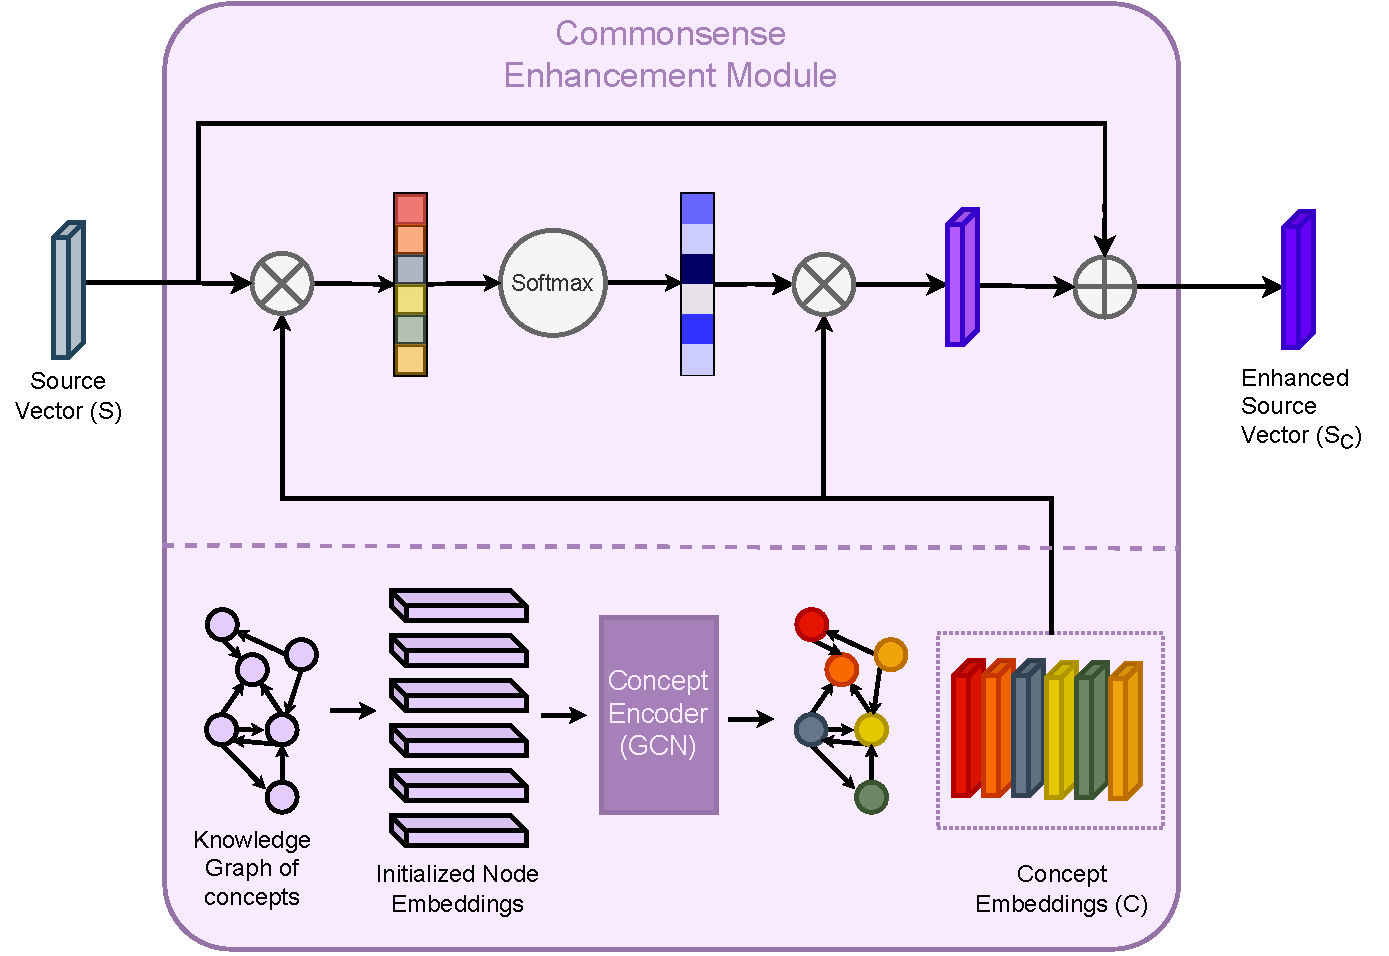
\includegraphics[width=0.8\linewidth]{figures/figure_files/Cem.pdf}
    \caption{\modelname Commonsense Enhancement Module (CEM). CEM comprises a concept encoder and an enhancement mechanism that uses the previously encoded concept vectors to update a given input vector (video/query vectors). The concept encoder employs a Graph Convolution Network for encoding the nodes (concepts) of \(G_C\). 
    }
  \label{fig:cem}
\end{figure}

CEM includes a set \(C\!=\!\left\{c_{1}, c_{2}, \dots, c_{n_{C}}\right\}\) of \(n_{C}\) concept vectors, where \(c_{i} \in \mathbb{R}^{d}\) and \(d\) is the concept feature dimension (same dimension as $\forall v_i \in V$ and $\forall q_i \in Q$). In general, given source feature vectors $S\!=\!\left\{ s_{1},s_{2},\ldots,s_{n}\right\}$ with individual feature vectors $s_{i \in [1,n]} \in \mathbb{R}^{d}$, the enhanced feature vectors $S_{C}$ are obtained using a commonsense enhancement mechanism $\phi_{C}$.
We implement this commonsense enhancement step $\phi_{C}$ as a cross-attention mechanism that enriches source input features, attending over $S$ guided by the commonsense concept vectors $C$, \ie, 
\begin{equation}
\label{eq:cenhance}
\scalemath{1}{
    }
    S_{C} = S + \phi_{C}(S) = S + \sigma \left( \frac{SW_{Q}(CW_{K})^{T}}{\sqrt{d}} \right) C W_{V},
\end{equation}
where $\sigma$ is a softmax activation, \(W_{Q}\), \(W_{K}\), \(W_{V}\) are trainable matrices and \(d\) is the common dimension of the vectors \(S\) and \(C\). In our setting, the source feature vectors $S$ are either video $V$ or pseudo-query $Q$ features. We build separate enhancement mechanisms for $V$ and $Q$, \ie, the projection matrices \(W_{Q}\), \(W_{K}\), \(W_{V}\) are not shared between $Q$ and $V$. We elaborate more on the rationale in the appendix.
The enriched video and pseudo-query features are denoted as \(V_{C}\!=\!\phi_{C_{\text{vid}}}(V)\) and \(Q_{C}\!=\!\phi_{C_{\text{pq}}}(Q)\), respectively.

\paragraph{Concept Encoder.}
The concept vectors \(C\) mentioned above are feature representations that internally form the nodes of the commonsense graph, \(G_C\). Accordingly, graph \(G_{C}\) is represented as a matrix, where \(G_{C(i,j)}\) represents the total number of directed relational edges between \(c_{i},c{j} \in C\) that start at \(c_i\) and end at \(c_j\). To encode the commonsense information, we employ Graph Convolutional Networks (GCN) \cite{hammond_wavelets_2011}. The concept encoder is composed of $L$ graph convolution layers, each of which performs a convolution step
\begin{equation}
\scalemath{1}{
    C^{\left(l+1\right)}=\sigma \left( AC^{\left(l\right) }W^{\left( l\right) }\right),
    }
\end{equation}
where $C^{\left(l\right)}$ are node (concept) features and $W^{\left( l\right)}$ trainable weight matrix of layer $l \in [1, L]$, $\sigma$ is a nonlinear activation function, and $A$ is the adjacency matrix obtained by normalizing graph $G_C$ with the degree matrix $D$. Since $G_C$ is a directed graph, normalization can be formulated as $A\!=\!D^{-1}G_{C}$.

\paragraph{Commonsense Information.}
We use ConceptNet \cite{speer_conceptnet_2017}, a popular knowledge graph that provides information spanning various types of relationships such as physical, spatial, behavioral, \etc To ensure that the ConceptNet information utilized is relevant to themes found in the video data, we consider the set of objects available in pseudo-queries and include the top-$k$ most frequently occurring objects to be the seed concept set \(C\). We extract the  ConceptNet subgraph that includes all edges incident between the concepts in \(C\). 
We filter the edge types based on a pre-determined relation set \(R\), which is compiled to involve relations that are relevant to the nature of the video localization task, \eg, spatial (\textit{AtLocation}, \etc) and temporal (\textit{HasSubevent}, \etc) relations are useful for video understanding, while \textit{RelatedTo} and \textit{Synonym} are fairly generic relations that add little information to the localization task. Table \ref{tab:relations} shows the relations included in \(G_C\).

\paragraph{Cross-Modal Interaction Module.} The commonsense enriched video and query features, \(V_{C}\) and \(Q_{C}\), are fused with a multi-modal cross-attention mechanism. We employ a two-step fusion process. First, Query-guided Video Attention (QVA) is applied to attend over video $V_C$, and Video-guided Query Attention (VQA) attends over query $Q_C$ guided by video $V_C$, resulting in updated features $V_C'$ and $Q_C'$, respectively. Both QVA and VQA utilize Attention Dynamic Filters~\cite{rodriguez_proposal-free_2020} that adaptively modify video features, dynamically adjusting them in response to the query, and vice versa. Next, the attended features are fused using a cross-attention mechanism over $V_C'$ guided by $Q_C'$, resulting in localized video features $V_{C_{\text{loc}}}$.

\paragraph{Temporal Regression Module.}
The final step involves a regression layer that approximates $\hat{V}_{\text{span}}$. We employ attention-guided temporal regression to estimate the span of the target video moment. To find important temporal segments relevant to the query, the fused features $V_{C_{\text{loc}}}$ are temporally attended based on the query features to obtain $V_{\text{ta}}$. Then, the span boundaries are localized using a regressor implemented as a Multi-Layer Perceptron (MLP).

\begin{align}
{o}_i = \sigma\left({W}_{1} V_{C_{\text{loc}_i}} + {b}_{{1}}\right) \\
V_{\text{ta}} = \sum_{i=1}^{T} o_i V_{C_{\text{loc}_{i}}} \\
[\hat{t}_s, \hat{t}_e] = {W}_2 {V}_{\text{ta}} + {b}_{2}.
\end{align}
Here, ${W}_{1}$ and ${b}_1$ are the weight matrix and bias vector of the temporal attention MLP, $\sigma$ represents the sigmoid activation function, $V_{C_{\text{loc}_i}}$ stands for the encoded localized video features, ${V}_{\text{ta}}$ represents the temporally attended video features, ${W}_2$ and ${b}_2$ denote the weight matrix and bias vector of the regression MLP, and $[\hat{t}_s, \hat{t}_e]$ correspond to the start and end timestamps of the predicted video span $\hat{V}_{\text{span}}$.

\begin{table}[t!]
\centering
\resizebox{\linewidth}{!}{
\begin{tabular}{ll}
\toprule
\textbf{Category} & \textbf{Relations}                                                                                         \\ \toprule
Spatial           & AtLocation, LocatedNear                                                                                    \\ \midrule
Temporal          & \begin{tabular}[c]{@{}l@{}}HasSubevent, HasFirstSubevent, HasLastSubevent, HasPrerequisite\end{tabular} \\ \midrule
Functional        & UsedFor                                                                                                    \\ \midrule
Causal            & Causes                                                                                                     \\ \midrule
Motivation        & MotivatedByGoal,  ObstructedBy                                                                             \\ \midrule
Other             & CreatedBy, MadeOf                                                                                          \\ \midrule
Physical          & \begin{tabular}[c]{@{}l@{}}HasA, HasProperty, Antonym, SimilarTo\end{tabular}                      
\\ \bottomrule
\end{tabular}
}

\caption{Relations in the Commonsense Enhancement Module (CEM) grouped by categories.}
\label{tab:relations}

\end{table}
\subsection{Training and Inference}
The training objective is 
$\mathcal{L}_{loc} = \mathcal{L}_{treg}+\lambda \mathcal{L}_{ta},$ where \(\lambda\) is a balancing hyperparameter, \(\mathcal{L}_{ta}\) is a temporal attention guided loss and \(\mathcal{L}_{treg}\) is the regression loss.  The temporal attention-guided loss is defined as
\begin{equation}
\label{tatt}
\mathcal{L}_{ta} = \frac{\sum^{T}_{i=1}g_{i}\log \left( a_{i}\right)}{\sum^{T}_{i=1}g_{i}},
\end{equation}
where \(a_{i}\) is the attention weight for video frame \(v_{i}\) and \(g_{i}\) is the attention mask for \(v_{i}\), that is assigned to \(1\) if \(v_{i}\) is inside the target video segment, and \(0\) otherwise. 
This objective encourages the model to produce higher attention weights for video segments that are relevant to the query. 
On the other hand, \(\mathcal{L}_{treg}\) dictates the video span boundary regression and is the sum of smooth $\ell_1$ distances between start and end timestamps of the ground truth and predicted spans, \ie,
\begin{equation}
\label{treg}
\mathcal{L}_{treg} = \text{smooth}{\ell_1}(t_{s}, \hat{t}_{s}) + \text{smooth}{\ell_1}(t_{e}, \hat{t}_{e}).
\end{equation}
Here, $t_{s}$ and ${t}_{e}$ represent the ground truth start and end timestamps and $\hat{t}_{s}$ and $\hat{t}_{e}$ the predicted start and end timestamps, respectively.
The integration of a smoothing mechanism enhances training stability and improves the model's ability to handle outliers. Finally, during inference, we employ an off-the-shelf part-of-speech tagger to extract nouns from the text input query and feed them as query input to the trained \modelname video localizer.
% \vspace{-1em}
\section{Neuro-Symbolic Theorem Proving}
\label{sec:softProlog}
% \vspace{-1em}
% As stated earlier, given the state $\state$, action $\action$ and goal $\goal$, we intend to prove the goal against a knowledge base $K$ such that the state and action appear in the proof path. This is how we filter-out irrelevant proofs. The variable groundings and the proof trace itself allows us to make informed decisions about the under specified user statements. For example, Figure \ref{fig:prooftree} shows the proof trace for ``if it snows at night then wake me up early because I want to get to work on time''. Traversing the proof trace allows CORGI to indicate the amount of precipitation to search for when checking the state $\state$ and also the meaning of ``early'' in the action $\action$ according to the user's commute time and traffic time.
Our Neuro-Symbolic theorem prover is a neural modification of \emph{backward chaining} and uses the vector similarity between rule and variable embeddings for unification.
In order to learn these embeddings, our theorem prover learns a general proving strategy by training on proof traces of successful proofs.
% The proving strategy that the model learns to mimic is \emph{backward chaining}. 
From a high level, for a given query our model maximizes the probability of choosing the correct rule to pick in each step of the backward chaining algorithm.
% Our system uses an embeddings-based approach to enable it to handle the variations typical to natural language settings. \textState $\state$, \textAction $\action$ and \textGoal $\goal$ are all extracted directly from user utterances, and may not exactly match anything in the knowledge base.
% The inference algorithm we use for extracting a relevant proof of $\goal$ is backward chaining. In what follows we explain our soft unification algorithm that learns
% Given a \textGoal to prove, backward chaining searches all the rules and facts in the knowledge base to find the ones whose head unify with the \textGoal. If unification succeeds for a rule, the algorithm moves on to prove the statements in the body of the rule in the same manner. If unification with a fact succeeds the proof terminates with a success. Since our rules and facts are extracted from natural language statements, there is a high chance that there is variation in the arguments and predicate names. For example, unification of \prologTerm{awake(i,early$\_$morning)} and \prologTerm{wake(me, early$\_$morning)} will fail using traditional backward chaining. Therefore, we propose a ``soft unification'' strategy to deal with these variations. \amoscomment{The information in this paragraph has appeared twice earlier, you can save some space here.}
% Our soft unification algorithm learns 
% embeddings for the prolog terms and uses vector similarity to make a decision about the success or failure of unification. In order to learn these embeddings, we collect proof traces and maximize the probability of extracting the correct proof for each query by walking down the proof path and maximizing the probability of choosing the correct rule next and making the correct variable groundings if any.
% \amoscomment{All these citations don't appear correctly in pdf.}
% \cite{rocktaschel2017end} and \cite{weber2019nlprolog} also propose a soft unification method, but they present soft ``AND'' and ``OR'' operations and propose a differentiable unification operator. 
This proposal is an adaptation of Reed et al.'s Neural Programmer-Interpreter \cite{reed2015neural} that learns to execute algorithms such as addition and sort, by training on their execution trace.

In what follows, we represent scalars with lowercase letters, vectors with bold lowercase letters and matrices with bold uppercase letters. %Amos: I don't really like the future tense, but not sure if this is really a problem. Forough: fixed it to present tense
% Our main observation is that we want to use the chain of reasoning -- proof trace in Prolog -- for a given statement to learn continuous representations for the facts and rules in the knowledge base.
% Given a state $\state$, and action $\action$ and a goal $\goal$ we want to indicate the $\theta$ for which a proof path in the knowledge base of facts $K$ exists. Formally:
% \amoscomment{Something is obviously missing here. Where is $\theta$ defined? I don't understand what it stands for.}
% \begin{equation}
%     S(X) \cap A_\theta(X) \cap K \rightarrow G_\theta{X}
% \end{equation}
% Our goal is to represent the backward chaining algorithm through a differentiable process similar to \cite{rocktaschel2017end}. Our approach is inspired by the neural program interpreter \citep{reed2015neural} where the authors use the program traces to execute a given program. Our goal here is to prove a statement given the complete proof trace.
% \facomment{consider using an RNN for embedding the rules}
$\mathbf{M}^{\text{rule}} \in \mathbb{R}^{n_1 \times m_1}$ denotes the embedding matrix for the rules and facts, where $n_1$ is the number of rules and facts and $m_1$ is the embedding dimension. 
% Row $i$ in $\mathbf{M}^{\text{rule}}$ corresponds to the $i^{\text{th}}$ rule/fact in the knowledge base $K$. 
$\mathbf{M}^{\text{var}} \in \mathbb{R}^{n_2 \times m_2}$ denotes the variable embedding matrix, where $n_2$ is the number of all the atoms and variables in the knowledge base and $m_2$ is the variable embedding dimension. 
% Each variable and atom has a corresponding row in the variable embedding matrix. 
Our knowledge base is type coerced, therefore the variable names are associated with their types (e.g., \prologTerm{alarm(Person,Time)})
% In the next subsection we present the learning algorithm for learning these embeddings and present the details of the model.
% We will represent the rules with two key-value matrices $M^{\text{key}} \in \mathbb{R}^{N \times K}$ and  $M^{\text{rule}} \in \mathbb{R}^{N \times M_1}$.  Variables are represented with an embedding matrix $V^{\text{var}} \in \mathbb{R}^{N \times M_2}$ and an attention over the embedding space  $V^{\text{key}} \in \mathbb{R}^{N \times K}$. 
% \mgcomment{Just an embedding matrix for both rules and variables, variable embedding matrix is initialized with gLoVe embeddings} Row $i$ in the $M$ matrices corresponds to rule $i$ in the knowledgebase, and row $i$ in the $V$ matrices corresponds to variable $i$ in the knowledgebase.
%\mgcomment{Could mention that all facts with a certain predicate are mapped to a common $\langle predicate\rangle/\langle arity\rangle$ embedding but rules have their own embedding} \facomment{debating whether we want to give this much detail}. 
%% We assume that we maintain and update a list of variables and predicates from the knowledgebase.
%% \amoscomment{I think that I undetsand this, but I thought that you are using Prolog. The standard Prolog obviously doesn't support all this, right? Or is all this only for selecting the rules to be used, but then the proof uses standard Prolog.} \facomment{that would be the inference algorithm. No we are not using standard prolog anywhere}
%\amoscomment{Can you please give an example here? What might be the an entry for a specific case, what does that entry actually mean?}\facomment{Is this still needed?}
% \vspace{-0.5em}
\paragraph{Learning}
% In this section, we present the model that takes as input a query to prove and returns a proof that consists of a sequence of rules and variable bindings. This model is adapted from \cite{reed2015neural}'s neural program interpreter that learns to execute programs and is trained on program execution traces. In this paper, we learn to complete proofs by training a model using proof traces.% \amoscomment{Again citations don't appear correctly. I think that citet doesn't work.}
The model's core consists of an LSTM network whose hidden state indicates the next rule in the proof trace and a proof termination probability, given a query as input. The model has a feed forward network that makes variable binding decisions. The model's training is fully supervised by the proof trace of a query given in a depth-first-traversal order from left to right (Fig.~\ref{fig:prooftree}). The trace is sequentially input to the model in the traversal order as explained in what follows. In step $t \in [0,T]$ of the proof, the model's input is $\epsilon^{inp}_t = \big(\mathbf{q}_t, \mathbf{r}_t, (\mathbf{v}^1_t, \dots, \mathbf{v}^\ell_t) \big)$ and $T$ is the total number of proof steps. $\mathbf{q}_t$ is the query's embedding and is computed by feeding the predicate name of the query into a character RNN. $\mathbf{r}_t$ is the concatenated embeddings of the rules in the parent and the left sister nodes in the proof trace, looked up from $\mathbf{M}^{rule}$. For example in Fig.\ref{fig:prooftree}, $\mathbf{q}_3$ represents the node at proof step $t=3$, $\mathbf{r}_3$ represents the rule highlighted in green (parent rule), and $\mathbf{r}_4$ represents the fact \prologTerm{alarm(i, 8)}. 
% We concluded empirically that it is critical to use both the parent and the left sister nodes in $r_t$. 
The reason for including the left sister node in $\mathbf{r}_t$ is that the proof is conducted in a left-to-right depth first order. Therefore, the decision of what next rule to choose in each node is dependent on both the left sisters and the parent (e.g. the parent and the left sisters of the node at step $t=8$ in Fig.~\ref{fig:prooftree} are the rules at nodes $t=1$, $t=2$, and $t=6$, respectively). 
% since both the sister nodes and the parent node are needed to make an informed decision about the next rule $r_{t+1}$ that should be chosen for the proof. 
% In order to compute $\mathbf{r}_t$, we concatenate the embeddings of the parent and sister nodes, which are looked up from $\mathbf{M}^{rule}$. 
The arguments of the query are presented in $(\mathbf{v}^1_t, \dots, \mathbf{v}^\ell_t)$ where $\ell$ is the arity of the query predicate. For example, $\mathbf{v}_3^1$ in Fig \ref{fig:prooftree} is the embedding of the variable \prologTerm{Person}. Each $\mathbf{v}^i_t$ for $i \in [0,\ell]$, is looked up from the embedding matrix $\mathbf{M}^{var}$. The output of the model in step $t$ is $\epsilon^{out}_t = \big(c_t, \mathbf{r}_{t+1}, (\mathbf{v}^1_{t+1}, \dots, \mathbf{v}^\ell_{t+1}))$ and is computed through the following equations
\begin{align}
    \mathbf{s}_t &= f_{enc}(\mathbf{q}_t,), ~~
    \mathbf{h}_t = f_{lstm}(\mathbf{s}_t, \mathbf{r}_t ,\mathbf{h}_{t-1}), \\
    c_t &= f_{end}(\mathbf{h}_t), ~~
    \mathbf{r}_{t+1} = f_{rule}(\mathbf{h}_t), ~~ %\label{eq:rt}
    \mathbf{v}^i_{t+1} = f_{var}(\mathbf{v}^i_t), \label{eq:ct} %\label{eq:vt},
\end{align}
where $\mathbf{v}^i_{t+1}$ is a probability vector over all the variables and atoms for the $i^{\text{th}}$ argument, $\mathbf{r}_{t+1}$ is a probability vector over all the rules and facts and $c_t$ is a scalar probability of terminating the proof at step t.
$f_{enc}$, $f_{end}$, $f_{rule}$ and $f_{var}$ are feed forward networks with two fully connected layers, and $f_{lstm}$ is an LSTM network. The trainable parameters of the model are the parameters of the feed forward neural networks, the LSTM network, the character RNN that embeds $\mathbf{q}_t$ and the rule and variable embedding matrices $\mathbf{M}^{rule}$ and $\mathbf{M}^{var}$.

Our model is trained end-to-end. In order to train the model parameters and the embeddings, we maximize the log likelihood probability given below
\begin{equation}
    {\bm \theta}^* = argmax~_{{\bm \theta}} \sum_{\epsilon^{out}, \epsilon^{in}} \log(P(\epsilon^{out} \vert \epsilon^{in};{\bm \theta})),
\end{equation}
where the summation is over all the proof traces in the training set and ${\bm \theta}$ is the trainable parameters of the model. We have
\begin{equation}
    \log(P(\epsilon^{out} \vert \epsilon^{in};{\bm \theta})) = \sum_{t=1}^T \log P(\epsilon^{out}_t \vert \epsilon^{in}_1 \dots \epsilon^{in}_{t-1}; {\bm \theta}), \\
\end{equation}
\begin{align}
    \log P(\epsilon^{out}_t \vert \epsilon^{in}_1 \dots \epsilon^{in}_{t-1}; {\bm \theta}) = & \log P(\epsilon^{out}_t \vert \epsilon^{in}_{t-1}; {\bm \theta}) \nonumber \\ 
     = & \log P(c_{t}\vert \mathbf{h}_t) +  \label{eq:probs}  \nonumber \\
     & \log P(\mathbf{r}_{t+1}\vert \mathbf{h}_t) + \nonumber \\
     & \log \sum_{i} P(\mathbf{v}^i_{t+1}\vert \mathbf{v}^i_t).
\end{align} 
% \end{equation}
% \begin{align}
%     \log P(\epsilon^{out}_t \vert \epsilon^{in}_1 \dots \epsilon^{in}_{t-1}; {\bm \theta}) & = \log P(\epsilon^{out}_t \vert \epsilon^{in}_{t-1}; {\bm \theta}) \\
%     & = \log P(c_{t}\vert \mathbf{h}_t) \label{eq:probs} + \nonumber \\
%     & ~~~~ \log P(\mathbf{r}_{t+1}\vert \mathbf{h}_t) +  \nonumber \\
%     & ~~~~  \log \sum_{i} P(\mathbf{v}^i_{t+1}\vert \mathbf{v}^i_t) 
% \end{align}
% \begin{align}
Where the probabilities in Equation \eqref{eq:probs} are given in Equations  \eqref{eq:ct}. The inference algorithm for porving is given in the Appendix, section Inference. %, \eqref{eq:rt} and \eqref{eq:vt}.
% Our learning algorithm uses the proof trace of different goals to learn the rule embedding and the variable embedding matrices. An example of the proof trace for a given goal is depicted in Figure \ref{fig:prooftree}. We optimize the log likelihood function 
% We present the input and output at each step of the proof with $\epsilon^{inp}_t = (q_t, r_t, v_t)$ where $q_t$ is the embedding of the query of the head of the rule \mgcomment{embedding of predicate of query} that is obtained through a character RNN, \amoscomment{Can you please provide more information on this character RNN? what was it trained to do (predict the next character?) what corpus was it trained on? (If it was taken from somewhere reference it).}
% $r_t$ is the embedding of the rule in this proof step \amoscomment{Where is this embedding obtained from?} 
%\mgcomment{$r\_t$ is a tuple of the embeddings of the parent rule and left sister rule in the proof tree or zero vector if not present for e.g. current_query: $food(X)$. parent_rule}
% and $v_t$ is the representation of the variables of the rule, which is obtained by a weighted average of the attention vector over the variable matrix. The output is $\epsilon^{out}_t = (v_{t+1}, r_{t+1}, c_t)$ where $c_t$ is the probability of proof completion. \amoscomment{I think that all this would be much easier to follow if reversed. First define the smaller pieces, then combine them.}
% We train the system such that we observe the output given the input for all the steps of the proof. More specifically:
% \facomment{no longer using $h_t$ for the variables}
% for inference and how to compute $h_t$ we have the following:
% where $q_0=[G(X), S(X), A(X)]$ and $q_t$ is the head of the rule at time $t$.
% \begin{align}
%     i^*_{rule} &= argmax~_{i=1\dots N} (M^{key}_{i,:})^T k_t \\
%     r_{t+1} &= M_{i*,:}^{rule} \\
%     v_{t+1} &= k_{t+1}^v V^{var} \label{eq:change}
% \end{align}
% \facomment{change \ref{eq:change} $k_{t+i} V_{t+1}$}
% \facomment{mention using GLOVE for initializing the variable embeddings}
% \facomment{predicates initialized randomly}
% \resizebox{0.7\textwidth}{!}{

% }
% % \section{Datasets}
We collected two sets of if-then-because commands.
% from human subjects (please refer to the Appendix for a more statistics). 
The first set contains 83 commands targeted at a \textState that can be observed by a computer/mobile phone (%which is
e.g. checking emails, calendar, maps, alarms, and weather). The second set contains 77 commands whose \textState is about day-to-day events and activities. 81\% of the commands over both sets qualify as ``if $\langle \text{\,\textState} \rangle $ then $\langle \text{\,\textAction} \rangle $ because $\langle \text{\,\textGoal} \rangle $''. The remaining 19\% differ in the categorization of the \textit{because}-clause (see Tab.~\ref{tab:statement_stats}); common alternate clause types included anti-goals (``...because I don't want to be late''), modifications of the state or action (``... because it will be difficult to find an Uber''), or conjunctions including at least one non-goal type. Note that we did not instruct the subjects to give us data from these categories, rather we uncovered them after data collection. 
% We selected only statements with goal-type because clauses for the work to follow but all the statements are released with the data. 
% \tmcomment{I suggest delete the next sentence}\facomment{removed} We would like to add that these commands are not to be used for training purposes, and are instead a benchmark task carefully designed and annotated to test machine common sense, defined as the ability of inferring hidden commonsense presumptions in if-then-because commands. 
% Note that
Also, commonsense benchmarks such as the Winograd Schema Challenge \cite{levesque2012winograd} included a similar number of examples (100) when first introduced \cite{kocijan2020review}.% and was scaled up very recently \cite{sakaguchi2019winogrande}.

Lastly, % after collecting the data we discovered that 
the if-then-because commands given by humans can be categorized into several different logic templates. 
% This is in contrary to the belief in the reasoning community that a single reasoning strategy could solve all reasoning problems, at least in a single benchmark. 
The discovered logic templates are given in Table \ref{tab:logic_templates} in the Appendix \footnote{The appendix is available at https://arxiv.org/abs/2006.10022}. Our neuro-symbolic theorem prover uses a general reasoning strategy that can address all reasoning templates. However, in an extended discussion in the Appendix, we explain how a reasoning system, including ours, could potentially benefit from these logic templates.

% \tmcomment{we don't really mean "when generating" commands do we in the next sentence?  Don't we mean that humans use different strategies to "reason about them"?   Also, doesn't it sound incorrect to claim that we know how humans reason?  Maybe delete this next paragraph except keep only the final sentence? } \facomment{ I changed it to the above, paragraph. (by the final sentence do you mean the sentence in line 12 of the latex source? or line 15 of the latex source?) Does it look good now?} After collecting the statements, we noticed that humans have different reasoning strategies when generating if-then-because commands. This is in contrary to the belief in the reasoning community that a single reasoning strategy could solve all reasoning problems, at least in a single benchmark.
% We believe this is a valuable finding because it indicates that researchers should perhaps consider these different reasoning strategies 
% shed some light on the different aspects of  what to consider when addressing reasoning problems. 
% The logic reasoning templates we discovered in the data are in Table \ref{tab:logic_templates} in the Appendix.
\vspace{-0.5em}
% We have further categorized the collected statements into four different logic templates listed in Tab.~\ref{tab:statement_stats}, right sub-table. The logic templates reflect how humans reason about if-then-because statements.
\section{Experiment Design}
% In this section, we provide the details of the model training and our experimental setup for testing the performance of CORGI.
The knowledge base, \KB, used for all experiments is a small handcrafted set of commonsense knowledge that reflects the incompleteness of SOTA KBs. See Tab.~\ref{tab:kb_examples} in the Appendix for examples and the code supplement to further explore our KB.
% as if-then rules, also known as horn clauses. 
\KB~includes general information about time, restricted-domains such as setting alarms and notifications, emails, and so on, as well as commonsense knowledge about day-to-day activities. \KB~contains a total of 228 facts and rules. Among these, there are 189 everyday-domain and 39 restricted domain facts and rules. We observed that most of the if-then-because commands require everyday-domain knowledge for reasoning, even if they are restricted-domain commands (see Table \ref{tab:dialog} for example). 
% Some examples of the facts and rules in the knowledge base are given below:

Our Neuro-Symbolic theorem prover is trained on proof traces (proof trees similar to Fig.~\ref{fig:prooftree}) collected by proving automatically generated queries to \KB~using sPyrolog\footnote{\url{https://github.com/leonweber/spyrolog}}. 
% Training queries were automatically generated from the predicates in \KB~(e.g. \prologTerm{isBefore(monday,?)}
% \kmcomment{TODO}\facomment{why is this a TODO? We have already done it}
% )% and proved using sPyrolog.
% that takes as input a similarity file crafted by the authors to bind semantically similar predicates and variables. 
$\mathbf{M}^{\text{rule}}$ and $\mathbf{M}^{\text{var}}$ are initialized randomly and with GloVe embeddings \cite{pennington2014glove}, respectively, where $m_1=256$ and $m_2=300$. Since \KB~is type-coerced (e.g. \prologTerm{Time}, \prologTerm{Location}, $\dots$), initializing the variables with pre-trained word embeddings helps capture their semantics and improves the performance. %rules-M1: 256, vars-M2: 300
% The embedding dimension of the variables is $300$ and the embedding dimension of the rules is $256$. 
The neural components of the theorem prover are implemented in PyTorch \cite{paszke2017automatic} and the prover is built on top of sPyrolog.%\footnote{Our code and data are available in the supplementary material}.
% [kmm - original text below:]
% Our rule embeddings were trained on proof traces collected from our knowledge base. The proof traces were collected by passing automatically-generated queries to sPyrolog. These queries were generated using the predicates in the knowledge base. The variable embedding matrix is initialized with GloVe embeddings \cite{pennington2014glove} and the rule embedding matrix is initialized randomly. Since the variable names refer to the variable type (e.g. \prologTerm{Time}, \prologTerm{Location}, $\dots$), it is important to initialize them with pre-trained word embeddings to capture their semantics. %rules-M1: 256, vars-M2: 300
% The embedding dimension of the variables is 300 and the embedding dimension of the rules is $256$. Our neural model and our soft reasoning system is implemented in PyTorch \cite{paszke2017automatic} and built on top of sPyroloy.
% Our knowledge base is a small hand crafted commonsense knowledge represented in terms of if-then rules, also known as horn clauses. This knowledge base includes general information about time and LIA-related contexts such as setting alarms and notifications, emails and so on, as well as open domain commonsense knowledge about day-to-day activities. This knowledge base consists of a total number of 228 facts and rules. Among these, there are 189 open-domain and 39 LIA-domain facts and rules. We observed that most of the statements require open-domain knowledge for reasoning, even if they are originally LIA-domain statements (see Figure \ref{fig:dialog} for example). Some examples of the facts and rules in the knowledge base are given below:
% \begin{itemize}
%     \item \prologTerm{isEarlierThan(Time1,Time2) :- isBefore(Time1,Time3), isEarlierThan(Time3,Time2).}
%     \item \prologTerm{isBefore(monday, tuesday).}
%     \item \prologTerm{notify(Person1, lia, Action1) :- email(Person1, Action1).}
% \end{itemize}
% [/kmm]

% \begin{align*}
%     \text{\prologTerm{isEarlierThan(Time1,Time2)}}  \text{\prologTerm{ :- isBefore(Time1,Time3),}}&  \\
%     \text{\prologTerm{isEarlierThan(Time3,Time2).}} & \\
%     \text{\prologTerm{isBefore(monday, tuesday).}}
% \end{align*}
\vspace{-0.5em}
\subsection{User Study}
% \begin{table}[ht]
    \caption{Number of successful reasoning tasks vs number of attempts under different scenarios. In CORGI's Oracle unification, soft unification is 100\% accurate. LT stands for Logic Template and LTi refers to template $i$ in Table \ref{tab:logic_templates}.}
    \label{tab:user_study_lt}
    \centering
    \resizebox{0.5\textwidth}{!}{%
    \begin{tabular}{lcccc}
    \toprule
    CORGI & \blueTemplate{LT1} & \orangeTemplate{LT2} & \greenTemplate{LT3} & \redTemplate{LT5} \\ \midrule
% Soft Unification & 0\% & 27\% & 24\% & 0\% \\
Oracle Unification & 24\% & 38\% & 11\% & 0\% \\
% \\
% No-feedback & 0/88 & 0/24 &  & & & \\
% Hard unification & ? & ? \\
% Soft unification & 16/88=18.18\% & 8/24= 33.33\% & 14\% & 37\% & 40\% & 52\% \\
% Soft unification & 16/88=18.18\% & 8/24= 33.33\% & 28\% & 21\% & 1\% & 4\% \\
% Soft unification & 26\% & 48\% & 4\% & 3\% \\
% Oracle unification & 20/77 = 25.97\% & 10/21 = 47.61\% \\
% \\
% Oracle unification & & & & \\
% \\
% Soft Unification (second batch) & 16/130 = 12.31\% & 3/10 = 30.00\% \\
% Soft Unification (second batch) & 23\% & 17\% & 2\% & 0\% \\
% Soft Unification (combined) & 22\% & 38\% & 4\% & 2\% \\
\bottomrule
    \end{tabular}
    }
\end{table}
\begin{table*}
\begin{minipage}{0.4\textwidth}
    \caption{percentage of successful reasoning tasks for different user types. In no-feedback, user responses are not considered in the proof attempt. in soft unification CORGI uses our proposed neuro-symbolic theorem prover. In the Oracle scenario, the theorem prover has access to oracle embeddings and soft unification is 100\% accurate.}
    \label{tab:user_study}
    \centering
    \resizebox{1\textwidth}{!}{%
    \begin{tabular}{lcc}
    \toprule
    CORGI variations & Novice User & Expert User  \\ \midrule
% No-feedback & 0/88 & 0/24 \\
No-feedback & 0\% & 0\% \\
% Hard unification & 15.61\% & 35\% \\
% Soft unification & 16/88=18.18\% & 8/24= 33.33\% & 14\% & 37\% & 40\% & 52\% \\
% Soft unification & 16/88=18.18\% & 8/24= 33.33\% & 28\% & 21\% & 1\% & 4\% \\
Soft unification & 15.61\% & 35.00\%  \\
% Oracle unification & 20/77 = 25.97\% & 10/21 = 47.61\% \\
% \\
Oracle unification & 21.62\% & 45.71\% \\
% Soft Unification (second batch) & 16/130 = 12.31\% & 3/10 = 30.00\% \\
% Soft Unification (second batch) & 12.31\% & 30.00\%  \\
% Soft Unification (combined) & 19.67\% & 52.5\% \\
\bottomrule
    \end{tabular}
    }
\end{minipage}
\!
\begin{minipage}{0.6\textwidth}
    % \captionof{figure}{\parbox{6.5cm}{Sample dialogs of 2 novice users in our study. CORGI's responses are noted in italics.}}
    \caption{\parbox{6.5cm}{Sample dialogs of 2 novice users in our study. CORGI's responses are noted in italics.}}
    \label{tab:dialog}
\centering
    \resizebox{0.95\textwidth}{!}{
    \begin{tabular}{p{1.7\columnwidth}}%{p{0.3\textwidth}}
    \toprule
    Successful task\\
    \midrule
    If it's going to rain in the afternoon then remind me to bring an umbrella because I want to remain dry.\\
    \hspace{2em}\textit{How do I know if ``I remain dry''?}\\
    If I have my umbrella.\\
    \hspace{2em}\textit{How do I know if ``I have my umbrella''?}\\
    If you remind me to bring an umbrella.\\
    \hspace{2em}\textit{Okay, I will perform ``remind me to bring an umbrella'' in order to achieve ``I remain dry''.}\\
    \\
    \toprule
    Failed task\\
    \midrule
    If it's going to rain in the afternoon then remind me to bring an umbrella because I want to remain dry.\\
    \hspace{2em}\textit{How do I know if ``I remain dry''?}\\
    If I have my umbrella.\\
    \hspace{2em}\textit{How do I know if ``I have my umbrella''?}\\
    If it's in my office.\\
    \hspace{2em}\textit{How do I know if ``it's in my office''?}\\
    ...
    \\
    \bottomrule
    \end{tabular}
    }
    % \rule{0.4\textwidth}{3cm}
    % \rule{0.8\textwidth}{3cm}
    % \label{fig:dialog}
\end{minipage}
% \vspace{-1em}
\end{table*}
In order to assess CORGI's performance, % and evaluate the effectiveness of the user feedback as well as the learned rule embeddings and the proposed soft reasoning 
we ran a user study. We selected 10 goal-type if-then-because commands from the dataset in Table \ref{tab:statement_stats} and used each as the prompt for a reasoning task.
We had 28 participants
% \footnote{Participants were not necessarily the people from whom we collected the dataset in Table \ref{tab:statement_stats}. Although it would be best to interact with the same user that inputs the statement, we argue that it is reasonable to use other humans for the explanations. First, most of these statements require day-to-day commonsense knowledge, therefore most humans will be able to give the required commonsense knowledge to the system. For example, some are as simple as having an umbrella to not get wet (Figure \ref{fig:dialog}). \kmcomment{I'm not convinced we need this paragraph; did a reviewer want it?}
% Second, we would like to be able to assess the performance of the model on a fixed dataset for comparison purposes. \kmcomment{I don't know what this means}}
in the study, 4 of which were experts closely familiar with CORGI and its capabilities. The rest were undergraduate and graduate students with the majority being in engineering or computer science fields and some that majored in business administration or psychology. These users had never interacted with CORGI prior to the study (novice users).
% The participants included students in the United States and Israel. 
Each person was issued the 10 reasoning tasks, taking on average 20 minutes to complete all 10. 

% We use a small subset of the if/then/because statements of Table \ref{tab:statement_stats} containing 10 examples and run a user study to assess the effectiveness of the user's feedback in proving the statements' because \textGoal and evaluate the performance of our proposed ``soft'' inference method. 14 people participated in our study and out of the 14 people, 3 were experts closely familiar with CORGI and its capabilities.
Solving a reasoning task consists of participating in a dialog with CORGI  as the system attempts to complete a proof for the \textGoal of the current task; 
% If the because \textGoal is not in the knowledge base, CORGI asks how to tell whether the goal has been achieved. 
% The user's responses are converted to new candidate if-then rules to add to \KB
% If the body of the rule is not found in the knowledge base, CORGI asks a new question, and so on
see sample dialogs in Tab.~\ref{tab:dialog}. The task succeeds if CORGI is able to use the answers provided by the participant to construct a reasoning chain (proof) leading from the \textGoal to the \textState and \textAction.
% If successful, CORGI adds all the candidate if-then rules to the knowledge base. If the system is not able to complete a proof after asking the user 3 questions, CORGI gives up and fails, discarding the candidate rules.
We collected 469 dialogues in our study.

The user study was run with the architecture shown in Fig.~\ref{fig:model}. 
We used the participant responses from the study to run a few more experiments. We (1) Replace our theorem prover with an \emph{oracle} prover that selects the optimal rule at each proof step in Alg.~\ref{alg:inference} and (2) attempt to prove the \textGoal without using any participant responses (\emph{no-feedback}). Tab.~\ref{tab:user_study} shows the success rate in each setting. % (1) Replace our theorem prover with vanilla prolog which does \emph{hard unification},
% Figure \ref{fig:dialog} shows examples of a successful vs. failed interaction with CORGI from the study.


% The results of the study are given in Table \ref{tab:user_study}. The fractions in the table indicate the number of successful reasoning tasks vs the number of attempted tasks. We compare the performance of CORGI against two scenarios. Scenario no-feedback is when we do not ask the users for any feedback and attempt to prove the because \textGoal against the knowledge base. The oracle scenario is when our soft unification has an oracle to select the optimal rule at each step so that soft unification always succeeds when it should and fails when it should.

% \amoscomment{reasons why it makes sense to ask other people to explain someone else's statements 1. they can better explain because when someone is too deep in the conversation then they cant give good feedback 2. if you crowdsource you will ask someone else to explain. 3. the 'explainers' may be better familiar with the engine's capabilities and knowledge.
% Clearly there is an advantage in asking the user to explain herself as she understands best what she wants.}

% \amoscomment{people need to understand what G(X) means}

% \amoscomment{at least 15 people in the user study}
% % %File: formatting-instruction.tex
% \documentclass[letterpaper]{article} % DO NOT CHANGE THIS
% \usepackage{aaai24}  % DO NOT CHANGE THIS
% \usepackage{times}  % DO NOT CHANGE THIS
% \usepackage{helvet}  % DO NOT CHANGE THIS
% \usepackage{courier}  % DO NOT CHANGE THIS
% \usepackage[hyphens]{url}  % DO NOT CHANGE THIS
% \usepackage{graphicx} % DO NOT CHANGE THIS
% \urlstyle{rm} % DO NOT CHANGE THIS
% \def\UrlFont{\rm}  % DO NOT CHANGE THIS
% \usepackage{natbib}  % DO NOT CHANGE THIS AND DO NOT ADD ANY OPTIONS TO IT
% \usepackage{caption} % DO NOT CHANGE THIS AND DO NOT ADD ANY OPTIONS TO IT
% \frenchspacing  % DO NOT CHANGE THIS
% \setlength{\pdfpagewidth}{8.5in}  % DO NOT CHANGE THIS
% \setlength{\pdfpageheight}{11in}  % DO NOT CHANGE THIS
% \usepackage{algorithm}
% % \usepackage{algorithmic}
% \usepackage{multirow}
% \usepackage{makecell}
% \usepackage{pifont}
% \usepackage{bbding}
% \usepackage{amsmath}
% \usepackage{amssymb}
% \usepackage{algpseudocode}
% \usepackage{booktabs}
% \usepackage{amstext}
% \usepackage{bm}
% \usepackage{subfigure}
% \newcommand{\eg}{\textit{e}.\textit{g}.}
% \usepackage{enumitem}
% \usepackage[table]{xcolor}

% \usepackage{url}            % simple URL typesetting
% \usepackage{booktabs}       % professional-quality tables
% \usepackage{mathtools,amssymb}
% \usepackage{amsfonts}       % blackboard math symbols
% \usepackage{nicefrac}       % compact symbols for 1/2, etc.
% \usepackage{microtype}      % microtypography
% \usepackage{pgfplots,pgfplotstable}
% \pgfplotsset{compat=1.14}
% \usepackage{array,colortbl}
% \usepackage{xcolor}
% \usepackage{algorithm,algorithmicx,algpseudocode}
% \usepackage[capitalise]{cleveref}
% \usepackage{caption}
% \usepackage{graphbox}
% \usepackage{placeins}
% % \usepackage{wrapfig}
% \usepackage{subcaption}
% \usepackage{etoolbox}

% \newcommand{\bzero}{\mathbf{0}}
% \newcommand{\bone}{\mathbf{1}}
% \newcommand{\bb}{\mathbf{b}}
% \newcommand{\bu}{\mathbf{u}}
% \newcommand{\bv}{\mathbf{v}}
% \newcommand{\bw}{\mathbf{w}}
% \newcommand{\bx}{\mathbf{x}}
% \newcommand{\by}{\mathbf{y}}
% \newcommand{\bz}{\mathbf{z}}
% \newcommand{\bxh}{\hat{\mathbf{x}}}
% \newcommand{\btheta}{{\boldsymbol{\theta}}}
% \newcommand{\bphi}{{\boldsymbol{\phi}}}
% \newcommand{\bepsilon}{{\boldsymbol{\epsilon}}}
% \newcommand{\bmu}{{\boldsymbol{\mu}}}
% \newcommand{\bnu}{{\boldsymbol{\nu}}}
% \newcommand{\bSigma}{{\boldsymbol{\Sigma}}}
% \newcommand{\vardbtilde}[1]{\tilde{\raisebox{0pt}[0.85\height]{$\tilde{#1}$}}}
% \newcommand{\defeq}{\coloneqq}
% \newcommand{\grad}{\nabla}
% \newcommand{\E}{\mathbb{E}}
% \newcommand{\Var}{\mathrm{Var}}
% \newcommand{\Cov}{\mathrm{Cov}}
% \newcommand{\Ea}[1]{\E\left[#1\right]}
% \newcommand{\Eb}[2]{\E_{#1}\!\left[#2\right]}
% \newcommand{\Vara}[1]{\Var\left[#1\right]}
% \newcommand{\Varb}[2]{\Var_{#1}\left[#2\right]}
% \newcommand{\kl}[2]{D_{\mathrm{KL}}\!\left(#1 ~ \| ~ #2\right)}
% \newcommand{\pdata}{{p_\mathrm{data}}}
% \newcommand{\bA}{\mathbf{A}}
% \newcommand{\bI}{\mathbf{I}}
% \newcommand{\bJ}{\mathbf{J}}
% \newcommand{\bH}{\mathbf{H}}
% \newcommand{\bL}{\mathbf{L}}
% \newcommand{\bM}{\mathbf{M}}
% \newcommand{\bQ}{\mathbf{Q}}
% \newcommand{\bR}{\mathbf{R}}

% \begin{document}
\onecolumn
\section{Appendix}

\subsection{Settings of PatchDiff}
The denoising step $T$ of our PatchDiff is $1000$, and the values of images and positional tensors are normalized into a range of $[-1, 1]$. We use AdamW optimizers with a initial learning rate of 1e-3 and a one-cycle learning rate scheduler. The weight decay strength is set to $0.0001$. The global noise $\epsilon_g$ is sampled from a global Gaussian distribution $mathcal{N}_g$ which has a standard deviation of $\sigma_g=0.02$ and every pixel has the identical noise vector. 

To better demonstrate the training and sampling differences between the PatchDiff and DDPM~\cite{DDPM}, we further present the algorithm details 
of training and sampling in Algorithm 1 and Algorithm 2. In particular, $\bepsilon_\theta$ is a function approximator intended to predict $\epsilon_1$ from $\bx_t$, $\epsilon_g$ is the global noise we introduced, and other variables are the same as in DDPM. Actually the sampling process is completely identical to the DDPM and without affected by the introducing of $\epsilon_g$ in the training stage.
\begin{figure}[!htpb]
\begin{minipage}[t]{0.495\textwidth}
\begin{algorithm}[H]
  \caption{Training} \label{alg:training}
  \small
  \begin{algorithmic}[1]
    \Repeat
      \State $\bx_0 \sim q(\bx_0)$
      \State $t \sim \mathrm{Uniform}(\{1, \dotsc, T\})$
      \State $\bepsilon_{1}\sim\mathcal{N}(\mathbf{0}, \mathbf{I}), \bepsilon_{g}\sim\mathcal{N}_g(\mathbf{0}, \sigma_g\mathbf{I})$
      \State Take gradient descent step on
      \State $\grad_\theta \left\| \bepsilon_1 - \bepsilon_\theta\bigl(\sqrt{\bar{\alpha}_t} \mathbf{x}_0 + \sqrt{1-\bar{\alpha}_t} \bepsilon_1 + \bepsilon_g, t\bigr) \right\|^2$
    \Until{converged}
  \end{algorithmic}
\end{algorithm}
\end{minipage}
\hfill
\begin{minipage}[t]{0.495\textwidth}
\begin{algorithm}[H]
  \caption{Sampling} \label{alg:sampling}
  \small
  \begin{algorithmic}[1]
    \vspace{.04in}
    \State $\bx_T \sim \mathcal{N}(\mathbf{0}, \mathbf{I})$
    \For{$t=T, \dotsc, 1$}
      \State $\bz \sim \mathcal{N}(\mathbf{0}, \mathbf{I})$ if $t > 1$, else $\bz = \mathbf{0}$
      \State $\bx_{t-1} = \frac{1}{\sqrt{\alpha_t}}\left( \bx_t - \frac{1-\alpha_t}{\sqrt{1-\bar\alpha_t}} \bepsilon_\theta(\bx_t, t) \right) + \sigma_t \bz$
    \EndFor
    \State \textbf{return} $\bx_0$
    \vspace{.04in}
  \end{algorithmic}
\end{algorithm}
\end{minipage}
% \vspace{-1em}
\end{figure}
% \vspace{0.2cm}

\subsection{Settings of Patch-based Detectors}
\subsubsection{Data augmentation}
We first present the data augmentation details applied during the training of detectors in MVTec AD and MVTec LOCO, as respectively illustrated in Table~\ref{tab:augmentation_mvtec} and Table~\ref{tab:augmentation_loco}, where $p$ denotes the probability of the images being with color jitter. It is worthy note that a larger color jitter range is applied for each generated set, which is expected to be helpful for learning color-level anomalies without training additional generators and detectors. (In principle, GRAD should expose the color-level structures by directly reduce the receptive field size of PatchDiff to 0 and generate pure noise images, then learn the color-level anomalies by level-1 detector)

\begin{table}[!htbp]
\centering
\renewcommand{\arraystretch}{1.}
\footnotesize
\resizebox{0.9\textwidth}{!}{
\begin{tabular}{lccccc}
\toprule
  &  &  &  & \multicolumn{2}{c}{Color jitter ($p=0.2$)} \\
\cmidrule{5-6}
Category  & Vertical flip & Horizontal flip & Random rotation ($\pm5^\circ$) & Normal data & Generated data\\
\midrule
Bottle  & \checkmark & \checkmark & \checkmark & $0.05$ & $0.5$\\
Cable  & \ding{55} & \ding{55} & \checkmark & $0.05$ & $0.5$\\
Capsule  & \ding{55} & \ding{55} & \checkmark &$0.05$ & $0.5$\\
Carpet  & \checkmark & \checkmark & \checkmark &$0.05$ & $0.5$\\
Grid  & \checkmark & \checkmark & \checkmark & $0.05$ & $0.5$\\
Hazelnut  & \checkmark & \checkmark & \checkmark & $0.05$ & $0.5$\\
Leather  & \checkmark & \checkmark & \checkmark & $0.05$ & $0.5$\\
Metal Nut  & \ding{55} & \ding{55} & \checkmark & $0.05$ & $0.5$\\
Pill  & \ding{55} & \ding{55} & \checkmark & $0.05$ & $0.5$\\
Screw  & \checkmark & \checkmark & \checkmark & $0.05$ & $0.5$\\
Tile  & \checkmark & \checkmark & \checkmark & $0.05$ & $0.5$\\
Toothbrush  & \ding{55} & \checkmark & \checkmark & $0.05$ & $0.5$\\
Transistor  & \ding{55} & \checkmark & \checkmark & $0.05$ & $0.5$\\
Wood  & \checkmark & \checkmark & \checkmark & $0.05$ & $0.5$\\
Zipper  & \checkmark & \checkmark & \checkmark & $0.05$ & $0.5$\\
\bottomrule
\end{tabular}}
\caption{Overview of the dataset augmentation techniques applied during training to each of the sub-dataset present in MVTec AD, similar to the setting as relative works~\cite{MVloco}.}
\label{tab:augmentation_mvtec}
\end{table}

\begin{table}[!htbp]
\centering
\footnotesize
\resizebox{1\textwidth}{!}
{
\begin{tabular}{lccccc}
\toprule
  &  &  &  & \multicolumn{2}{c}{Color jitter ($p=0.2$)} \\
\cmidrule{5-6}
Category  & Vertical flip & Horizontal flip & Random rotation ($\pm5^\circ$) & Normal data & Generated data\\
\midrule
Breakfast Box  & \ding{55} & \ding{55} & \checkmark & $0.05$ & $0.5$\\
Screw Bag & \checkmark & \checkmark & \checkmark & $0.05$  & $0.5$\\
Pushpins & \checkmark & \checkmark & \checkmark & $0.05$  & $0.5$\\
Splicing Connectors & \checkmark & \checkmark & \checkmark & $0.05$  & $0.5$\\
Juice Bottle & \ding{55} & \ding{55} & \checkmark & $0.05$  & $0.5$\\
\bottomrule
\end{tabular}}
\caption{Overview of the dataset augmentation techniques applied during training to each of the sub-dataset present in MVTec LOCO, similar to the setting as relative works~\cite{MVloco}.}
\label{tab:augmentation_loco}
\end{table}

\begin{table}[!htpb]
\centering
\footnotesize
\begin{tabular}{lcccc}
\toprule
Dataset     &Detector level & \makecell{Practical size of\\receptive field} & input size & PatchDiff level\\
\midrule
MVTec AD                       & 34    & $34\times34$  & $256\times256$   & 5, 9, 13   \\
\midrule
\multirow{3}{*}{MVTec LoCo AD} & 34    & $34\times34$  & $256\times256$   & 5, 9, 13   \\
                               & 68    & $34\times34$  & $128\times128$   & 5, 9, 13   \\
                               & 136   & $34\times34$  & $64\times64$     & 9, 13, 17 \\
\bottomrule    
\end{tabular}
\caption{The level configures list for patch-level detectors.}
\label{tab: GRad_level_configs}
% \vspace{-0.2cm}
\end{table}

\subsubsection{Training Detail} We then present the configuration details of the patch-level detectors across various levels, as outlined in Table \ref{tab: GRad_level_configs}. In the case of the MVTec AD dataset, we exclusively train a level-$34$ patch-level detector for each sub-dataset. In addition, for MVTec LOCO, we developed three detectors — each corresponding to level-$34$, $68$, and $136$ within their respective sub-datasets. Concerning these levels, the images are resized to dimensions of $256\times256$, $128\times128$, and $64\times64$ respectively. This resizing strategy allows us to maintain the practical receptive field size of each detector at $34\times34$, while the effective receptive field relatively expands to $34\times34$, $68\times68$, and $136\times136$ for the level-$34$, $68$, and $136$ detectors respectively. Moreover, the level-$34$ and $68$ patch-level detectors employ contrastive images generated by level-$5$, $9$, and $13$ PatchDiffs, whereas the level-$136$ patch-level detector employs contrastive images generated by level-$9$, $13$, and $17$ PatchDiffs. This meticulous selection of contrastive images from varying levels PatchDiff further contributes to the detectors' adeptness in capturing diverse local anomaly patterns. Moreover, for our reweighting mechanism, we introduce a memory bank size of 512 for storing the normal features during the training phase. We train the detector for 2000 epochs using AdamW with a one-cycle learning rate scheduler and an initial learning rate of 1e-3.

\begin{table}[!htpb]
\centering
\footnotesize
\begin{tabular}{cccccc}
\toprule
Layer Name & Stride & Kernel Size & Number of Kernels & Padding & Activation \\
\midrule
Conv-1 & 2$\times$2 & 4$\times$4 & 64 & 0 & ReLU \\
Conv-2 & 2$\times$2 & 4$\times$4 & 128 & 0 & ReLU \\
Conv-3 & 1$\times$1 & 3$\times$3 & 256 & 0 & ReLU \\
Conv-4 & 1$\times$1 & 3$\times$3 & 512 & 0 & ReLU \\
Conv-5 & 1$\times$1 & 3$\times$3 & 256 & 0 & ReLU \\
Conv-6 & 1$\times$1 & 1$\times$1 & 256 & 0 & ReLU \\
Conv-7 & 1$\times$1 & 1$\times$1 & 256 & 0 & ReLU \\
Conv-8 & 1$\times$1 & 1$\times$1 & 1 & 0 & - \\
\bottomrule
\end{tabular}
\caption{Network architecture of our patch-level detector.}
\label{tab: arch_detector}
\end{table}

\begin{table}[!htpb]
\centering
\footnotesize
% \resizebox{0.75\textwidth}{!}{
\begin{tabular}{cccccc}
\toprule
Layer Name & Stride & Kernel Size & Number of Kernels & Padding & Activation \\
\midrule
Conv-1 & 1$\times$1 & 1$\times$1 & 256 & 0 & ReLU \\
Conv-2 & 1$\times$1 & 1$\times$1 & 256 & 0 & ReLU \\
Conv-3 & 1$\times$1 & 1$\times$1 & 256 & 0 & ReLU \\
Conv-4 & 1$\times$1 & 1$\times$1 & 5780 & 0 & - \\
\bottomrule
\end{tabular}
\caption{Network architecture of MLP-based decoder for our regularization on features.}
\label{tab: arch_decoder}
\end{table}

\subsubsection{Network Architecture} Additionally, we illustrate the network architecture of our patch-level detector in Table~\ref{tab: arch_detector}, which outputs $1\times1$ anomaly score for an input patch size of $5\times34\times34$ pixels. Consequently, each individual patch-level detector encompasses around 2.9 million parameters, equipped with only 8 fully convolutional layers. Even though we integrate the comprehensive performance of three detectors for MVTec LOCO, the whole number of parameters is still only 8.7 million parameters, highlighting its lightweight structure when compared to prevailing backbone architectures as shown in first figure of our paper. Moreover, in Table~\ref{tab: arch_decoder}, we further illustrate the network architecture of MLP-based network for our regularization on features. We resize the output size $5780$ into $5\times34\times34$ pixels to achieve the reconstruction for the features encoded by our detectors. 

\subsection{Additional Experiment Results}
\subsection{Anomaly Generation}
Furthermore, as shown in Fig.~\ref{fig: mvtec_generation}, we present the samples of contrastive images generated by level-13 PatchDiff for MVTec AD.

\begin{figure*}[!h]
    \centering
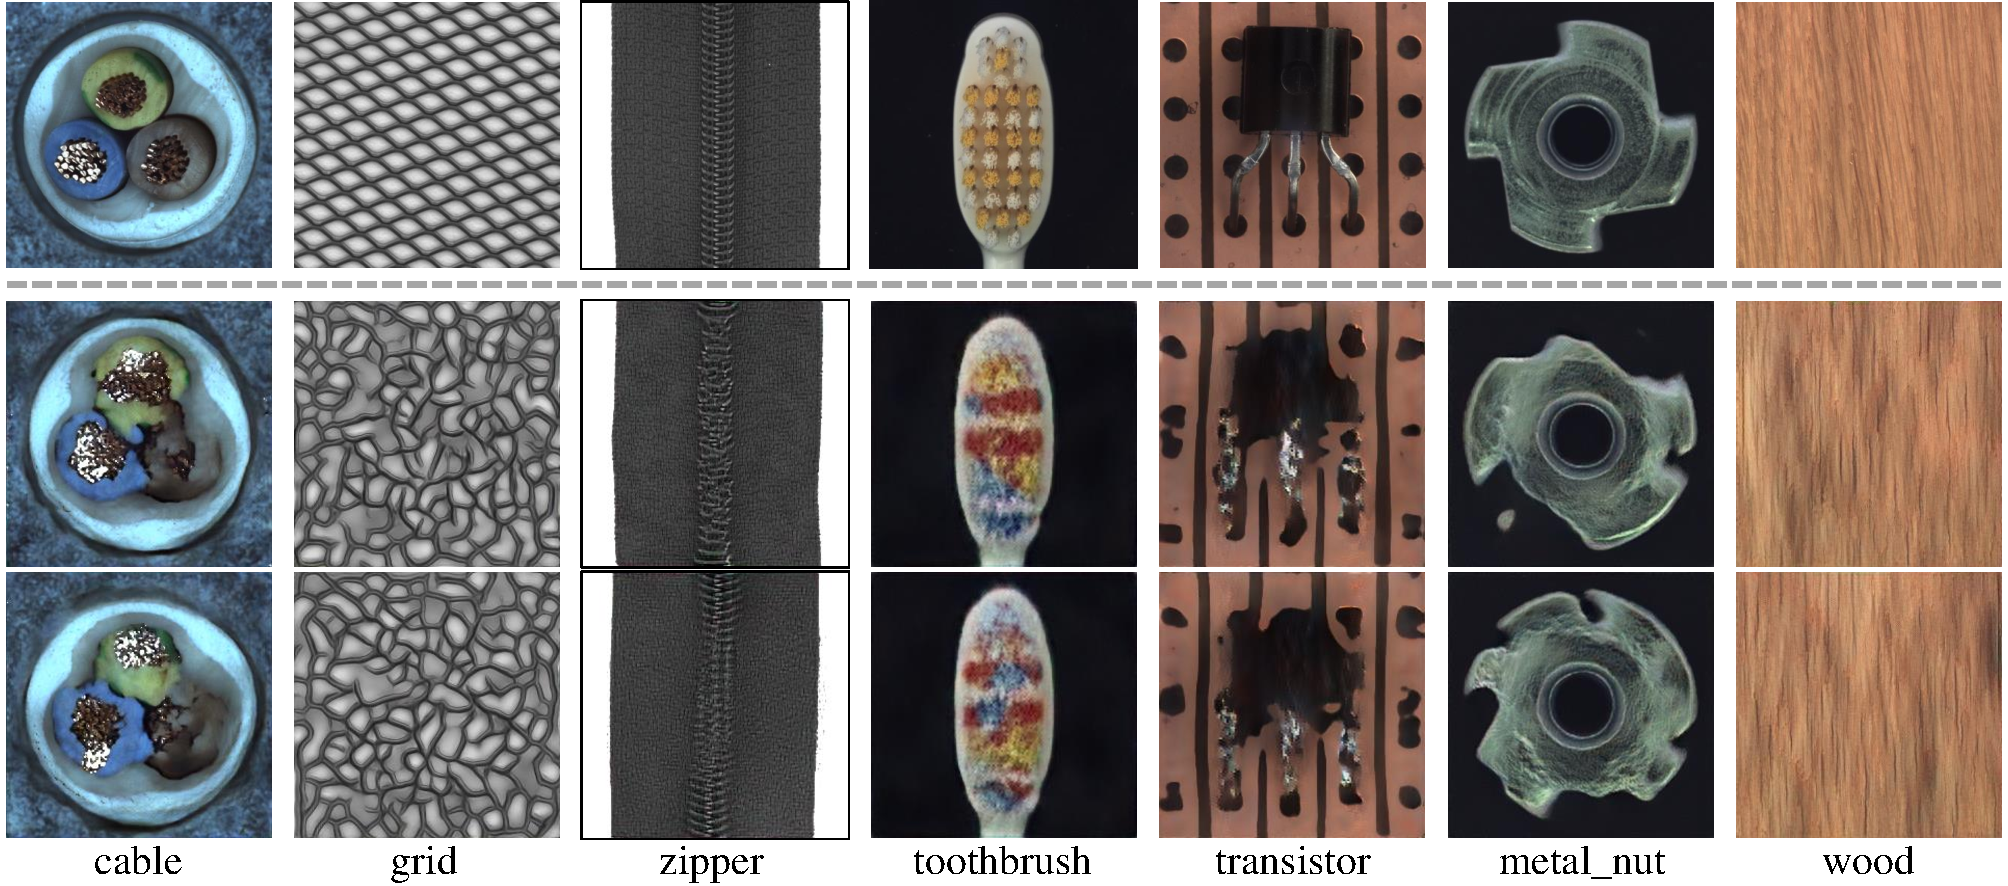
\includegraphics[width=0.7\linewidth]{images/mvtec_generation_results.pdf}
    \caption{Contrastive images generated by level-13 PatchDiff for MVTec AD~\cite{MVTecAD}. } 
    \label{fig: mvtec_generation}
\end{figure*}

\begin{table*}[!h]
    \centering
    % \footnotesize
    % \setlength{\belowcaptionskip}{0.2cm}
    % \setlength{\abovecaptionskip}{0.0cm}
    \renewcommand{\arraystretch}{1.2}
    \resizebox{\textwidth}{!}
    {
\begin{tabular}{cl|c|c|c|c|c|c|c|c}
\toprule
% \multicolumn{2}{c|}{Category} & \makecell[c]{IGD\\\tiny{\citealp{IGD}}} & \makecell[c]{PSVDD\\\tiny{\citealp{PSVDD}}} & \makecell[c]{FCDD\\\tiny{\citealp{FCDD}}} & \makecell[c]{CutPaste\\\tiny{\citealp{CutPaste}}} & \makecell[c]{NSA\\\tiny{\citealp{NSA}}} & \makecell[c]{DRAEM\\\tiny{\citealp{DRAEM}}} & \makecell[c]{DSR\\\tiny{\citealp{DSR}}} & \makecell[c]{GRAD\\\tiny{Ours}} \\ \midrule
\multicolumn{2}{c|}{Category}     & IGD & PSVDD & FCDD & CutPaste &NSA & DRAEM & DSR & GRAD \\ \midrule
\multirow{5}{*}{Texture} 
& carpet & (94.7, 82.8 ) & (92.9, 92.6) & (96.0, - ) & (93.1, 98.3) & (95.5, 95.6) & (95.5,97.0) & (-, \textbf{100.}) & (\textbf{96.5}, 98.2) \\
& grid & (97.7, 97.8 ) & (94.6, 100.) & (91.0, - ) & (\textbf{99.9}, 97.5) & (99.2, 99.9) & (99.7, 99.9) & (-, \textbf{100.}) & (97.2, \textbf{100.}) \\
& leather & (99.5, 95.8) & (90.9, 98.6) & (98.0, - ) & (\textbf{100.}, 99.5) & (99.5, 99.9) & (98.6, \textbf{100.}) & (-, \textbf{100.}) & (98.8, \textbf{100.}) \\
& tile & (78.0, 99.1) & (97.8, 91.4) & (91.0, - ) & (93.4, 90.5) & (\textbf{99.3}, \textbf{100.}) & (99.2, 99.6) & (-, \textbf{100.}) & (95.4, \textbf{100.}) \\
& wood & (89.1, 94.6) & (96.5, 90.8) & (88.0, - ) & (\textbf{98.6}, 95.5) & (90.7, 97.5) & (96.4, \textbf{99.1}) & (-, 96.3) & (87.2, 98.3) \\
\midrule
\multirow{10}{*}{Object} 
& bottle & (92.2, \textbf{100.}) & (98.6, 98.1) & (97.0, - ) & (98.3, 97.6) & (98.3, 97.7) & (\textbf{99.1}, 99.2) & (-, \textbf{100.}) & (96.5, \textbf{100.}) \\
& cable & (84.7, 90.6) & (90.3, 96.8) & (90.0, - ) & (80.6, 90.0) & (96.0, 94.5) & (94.7, 91.8) & (-, 93.8) & (\textbf{98.4}, \textbf{99.3}) \\
& capsule & (\textbf{97.7}, 91.5) & (76.7, 95.8) & (93.0, - ) & (96.2, 97.4) & (97.6, 95.2) & (94.3, \textbf{98.5}) & (-, 98.1) & (97.1, 96.4) \\
& hazelnut & (98.0, 99.7) & (92.0, 97.5) & (95.0, - ) & (97.3, 97.3) & (97.6, 94.7) & (\textbf{99.7}, \textbf{100.}) & (-, 95.6) & (96.6, 98.1) \\
& metal nut & (92.6, 91.3) & (94.0, 98.0) & (94.0, - ) & (99.3, 93.1) & (98.4, 98.7) & (\textbf{99.5}, 98.7) & (-, 98.5) & (93.7, \textbf{100.}) \\
& pill & (97.3, 87.3) & (86.1, 95.1) & (81.0, - ) & (92.4, 95.7) & (\textbf{98.5}, \textbf{99.2}) & (97.6, 98.9) & (-, 97.5) & (98.1, 95.7) \\
& screw & (97.0, 82.5) & (81.3, 95.7) & (86.0, - ) & (86.3, \textbf{96.7}) & (96.5, 90.2) & (97.6, 93.9) & (-, 96.2) & (\textbf{99.2}, 96.0) \\
& toothbrush & (97.7, 99.7) & (\textbf{100.}, 98.1) & (94.0, - ) & (98.3, 98.1) & (94.9, \textbf{100.}) & (98.1, \textbf{100.}) & (-, 99.7) & (98.0, 99.7) \\
& transistor & (84.4, 90.6) & (91.5, 97.0) & (88.0, - ) & (95.5, 93.0) & (88.0, 95.1) & (90.9, 93.1) & (-, 97.8) & (\textbf{97.8}, \textbf{100.}) \\
& zipper & (96.7, 97.0) & (97.9, 95.1) & (92.0, - ) & (\textbf{99.4}, 99.3) & (94.2, 99.8) & (98.9, \textbf{100.}) & (-, \textbf{100.}) & (98.3, 99.7) \\
\midrule
\multicolumn{2}{c|}{Average} & (93.1, 93.4) & (92.5, 93.2 ) & (92.1, 95.7) & (95.2, 96.0) & (96.3, 97.2) & (\textbf{97.3}, 98.0) & (-, 98.2) & (96.8, \textbf{98.7}) \\
\bottomrule
\end{tabular}}
\caption{Anomaly detection performance on MVTec AD dataset~\cite{MVTecAD}. Both pixel-level (left) and image-level (right) AUROC results are shown in each column. The best results are in bold.}
\label{tab: mvtec_main_detail}
\end{table*}

\subsection{Anomaly Detection and Localization}
In the main body, we exclusively present the averaged performance comparison on MVTec AD. In this section, we extend our analysis to provide a detailed result of the anomaly detection and localization performance across each individual sub-dataset within MVTec AD, and display anomaly maps on MVTec AD in Fig.~\ref{fig: main_mvtec_ad_results}. As shown in Table~\ref{tab: mvtec_main_detail}, we compare GRAD to IGD~\cite{IGD}, PSVDD~\cite{PSVDD}, FCDD~\cite{FCDD}, CutPaste~\cite{CutPaste}, NSA~\cite{NSA}, DRAEM~\cite{DRAEM}, and DSR~\cite{DSR}, all of which are independent of pretrained feature extractors. It is easy to find GRAD achieves a strong detection and localization of anomalies.  

\begin{figure*}[!h]
    \centering
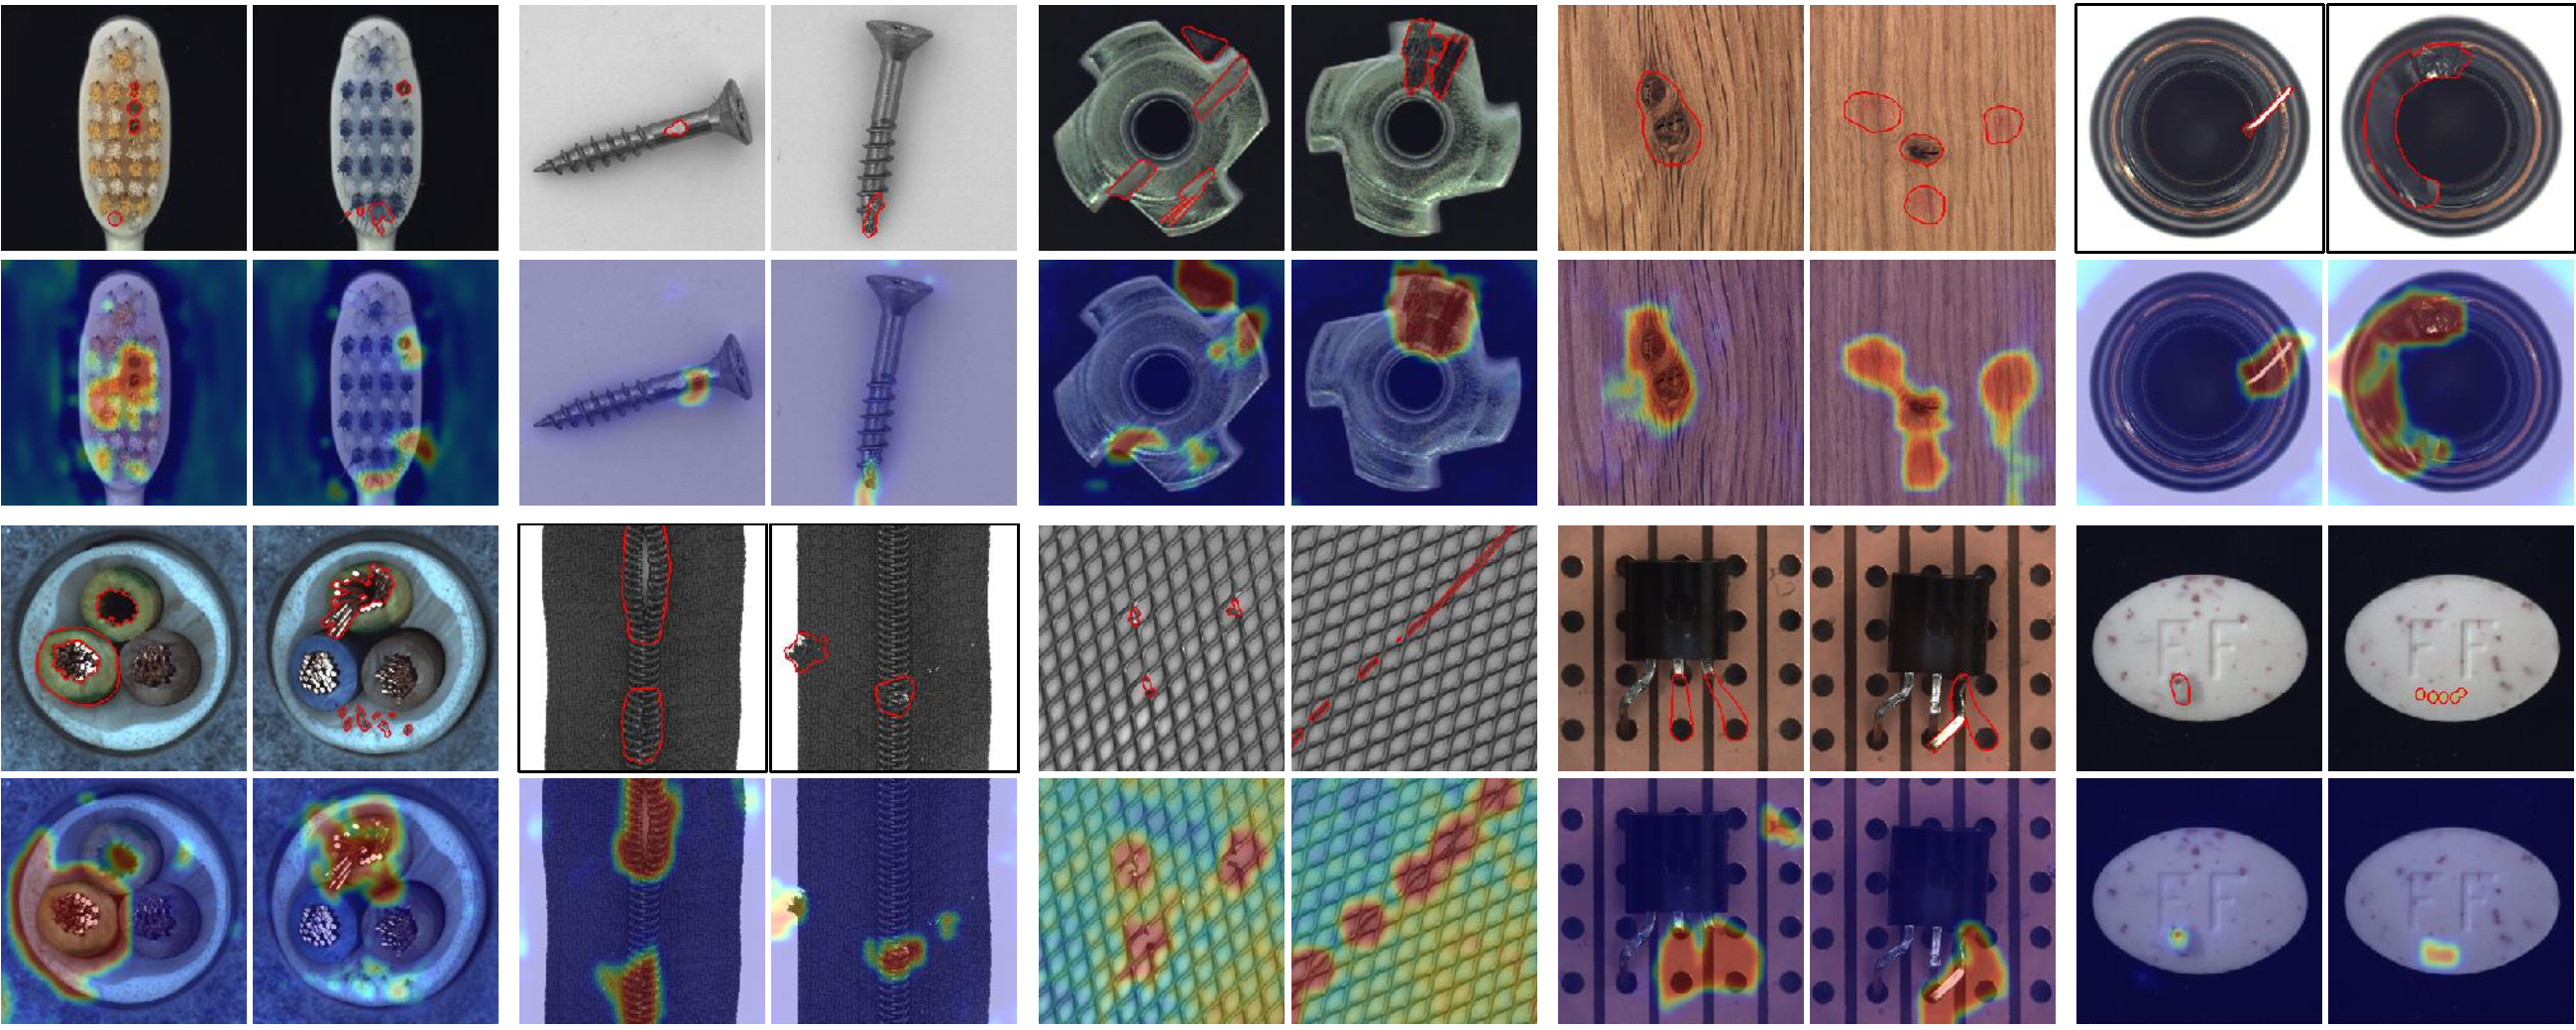
\includegraphics[width=0.9\linewidth]{images/mvtec_results.pdf}
    \caption{Defect localization results of GRAD on MVTec AD~\cite{MVTecAD}. } 
    \label{fig: main_mvtec_ad_results}
    % \vspace{-0.2cm}
\end{figure*}


% In addition, as shown in Table~\ref{tab:ablation_GRad_level}, we conduct an ablations study on selecting levels of patch-level detectors. It is easy to find that when integrating all three different levels of detectors, GRAD can achieve a strong performance for the detection of structural as well as logical anomalies.

% \begin{table}[!htbp]
% \centering
% \footnotesize
% \resizebox{0.3\textwidth}{!}{
% \begin{tabular}{ccc|c}
% \toprule
% \multicolumn{3}{c|}{Level Settings}& Image-level \\
% 136 & 68 & 34  & AUROC\\
% \midrule
% \checkmark &   \ding{55} & \ding{55}   &  85.2   \\
% \ding{55}& \checkmark & \ding{55} & 85.4 \\
% \ding{55}&\ding{55} & \checkmark & 75.1\\
% \checkmark & \checkmark & \ding{55}   &  86.8     \\ %
% \checkmark &   \ding{55} & \checkmark   &  86.4   \\
% \ding{55} & \checkmark & \checkmark  & 86.2 \\
% \checkmark & \checkmark & \checkmark &  \textbf{87.5}  \\
% \bottomrule
% \end{tabular}}
% \caption{Ablation study on detector levels. Detection AUROC results on MVTec LOCO dataset. The best results are in bold.}
% \label{tab:ablation_GRad_level}
% \end{table}



% \bibliography{aaai24}
% \bibliographystyle{aaai24}

% \end{document}


\section{Discussion}\label{sec:discussion}
%<insert>
%In this section we discuss the helpfulness of a theoretical ``audit standard'' to study content curators and note how our framework might contribute to such a standard. We also note the various audit methods used in this study and clarify the strengths of the different methods. In regards to the audit results, we discuss possible motivations for the mechanism design 
In this section we first discuss the specific results found in our audit of Apple News and how our results paint a distinction between algorithmic logic and human editorial logic. We then consider the broader implications of our study in terms of the various audit methods used, clarifying their different strengths. And finally, we suggest that the audit framework we develop may contribute to informing a conceptual ``audit standard'' which helps make the questions and methods more consistent when approaching similar audits of other news curators. 


\subsection{Mechanisms behind Apple News}
The absence of localization and personalization in the sections we audited highlights a possible tension between equitable economic distribution and vulnerability to echo-chambers. By showing the same Top Stories and Trending Stories to every user, Apple has taken a measure that minimizes individual filter bubble effects. However, this design choice may also translate to a highly-skewed distribution of economic winnings for publishers, since the few sources that frequent the top slots reap disproportionate traffic and potential advertising revenue from the 85 million users. 

Certainly, a balance could mitigate filter bubble effects while creating more equitable monetization. For example, Google News provides all users with an algorithmically-selected five-story briefing, but the same two top stories are shown to all users \citep{Wang2018}. Apple might explore a similar hybrid approach, using their editorial team to choose a mix of regionally and nationally relevant news. It should also be noted that Apple News includes a ``For You" section based on ``topics \& channels you read," which may help balance these tensions. 


\subsection{Algorithmic vs. Editorial Logic}
Our results illustrate what \citet{Gillespie2014} refers to as a possible competition between ``editorial logic'' and ``algorithmic logic.'' While the algorithmic logic behind Trending Stories is intended to ``automate some proxy of human judgment or unearth patterns across collected social traces,'' the editorial logic behind Top Stories ``depends on the subjective choices of experts, themselves made and authorized through institutional processes of training and certification'' \citep{Gillespie2014}. These logics manifest in our audit results for both mechanism and  content: Trending Stories and Top Stories exhibit distinct update schedules, sources, and topics that reflect their respective logics.

According to interviews with Apple's staff by \citet{Nicas2018}, the editorial logic behind the Top Stories pushes new content ``depending on the news,'' and also ``prioritizes accuracy over speed.'' In contrast, the Trending Stories section continually churns out new content (over 50 stories per day on average, more than twice as many as the Top Stories section). The algorithmic logic continually updates `what's trending,' and does so at all hours of the day (see Figure \ref{fig-trending-stories-appearance-times}), whereas the editorial logic espoused by Apple's staff strives for ``subtly following the news cycle and what's important'' \citep{Nicas2018}.

The contrast in logics extends to source concentration and source diversity. The editorially-selected Top Stories section exhibited more diverse and more equitable source distribution than the algorithmically-selected Trending Stories, as detailed in Table \ref{summary-table} and visualized in Figures \ref{fig-trending_stories_distribution} and \ref{fig-top_stories_distribution}. During the two-month data collection, human editors chose from a slightly wider array of sources than the algorithm behind Trending Stories, and also distributed selections more equitably across those sources, although there was a core set of 40 sources that were selected by \textit{both} algorithm and editor. Apple's editors also appeared to seek out regional news sources when the topic called for it. For example, during our data collection, the team chose stories from The San Diego Union-Tribune, The Miami Herald, The Chicago Tribune, TwinCities.com, and The Baltimore Sun. While the Trending Stories algorithm surfaced some content from smaller sources (e.g., esimoney.com, a single-author website dedicated to money management), no sources were regionally-specific.

Finally, perhaps the most intuitive distinction between the editorial logic and the algorithmic logic exhibited in Apple News is differences in content. Trending Stories uniquely included ``soft news'' \citep{Reinemann2012} pieces about celebrities and entertainment (ex. Kate Middleton, Justin Bieber), while the Top Stories uniquely included ``hard news'' topics including international stories and news about political policy (ex. Brexit, Affordable Care Act). Our data corroborates initial reports that headlines in Trending Stories ``tend to focus on Mr. Trump or celebrities'' \citep{Nicas2018}.


\subsection{Broader Implications}

\subsubsection{Audit Methods}
To study Apple News we used scraping, sock-puppet, and crowdsourced auditing. While these techniques have been employed in previous audit studies, we next reflect on our experience of how we found each technique helpful for addressing different aspects of our audit framework, in hopes this can inform future audit studies. 

First, audit studies should consider crowdsourcing whenever real-world observation is important, or when seeking higher parallel throughput in the data collection process. By using the crowd, we were able to assess the degree of personalization Apple News performs in practice, rather than fully relying on simulated sock-puppet data. Also, since resource constraints limited us to run at most two simulators at a time, crowdsourcing allowed us to significantly increase the throughput of our data collection, as many crowd workers could take screenshots in parallel.

Sock-puppet auditing -- using computer programs to impersonate users \citep{Sandvig2014} -- is most helpful for isolating variables that might affect a given system. Sock puppets provide clear and precise information about the input to an algorithm in cases where the crowd falls short. For example, precise temporal synchronization was still challenging with crowdworkers, as 6.7\% of screenshots from the crowd showed times that did not match the requested time in minutes, and even screenshots at the correct hour and minute may have been unsynchronized if seconds were taken into account. On the other hand, when using sock puppets, we could perform time-locked data collection on multiple devices with same-second precision.
%fine-grained location reporting is invasive: in a pilot study we attempted collecting ZIP codes, which some crowd workers either forged or simply declined to report. However, when using sock puppets, we could precisely situate the device at a given latitude and longitude while guaranteeing the absence of other factors such as user-level blocked sources. 

Lastly, we found the scraping audit most helpful for extended data collection, and we suggest scraping whenever researchers seek continuous data or to monitor over time. While we initially deployed a crowdsourced method for the extended data collection \citep{Bandy}, we found that we could not rely on the crowd for consistent data over time. Namely, in the United States, it was difficult to collect screenshots between the hours of 1am and 5am. However, after observing no evidence of personalization or localization in our initial experiments, we needed data from just one user account. We could therefore scrape content from a single simulated device to run the extended data collection.

It should be noted that we categorize our Appium-based data collection as a scraping audit since it centers around ``repeated queries to a platform and observing the results'' \citep{Sandvig2014}, however, we used a simulated iPhone to impersonate a user, making it somewhat of a hybrid with sock-puppet auditing. The Apple News platform lacks a public or private endpoint from which to scrape stories, so our experiment required additional layers of operation -- every data point we collected required simulating a user opening the application, refreshing for new content, locating buttons, and pressing buttons, thus requiring more time to collect data compared to a traditional scrape.

\subsubsection{Audit Framework}
To guide this work, we developed a conceptual framework that articulates three common aspects of a curation system that an audit might address: mechanism, content, and consumption. We showed how each of these aspects can have consequences for individual users, publishing companies, and even political discourse. As news curation systems change, consequential aspects may also change and prompt an expanded or revised framework.

Still, future research might leverage our proposed framework for auditing other content curators, revising and elaborating it to suit the nuances of specific systems. We believe this framework helps advance towards a conceptual ``audit standard'' for curation systems, which might allow the research community to compare and contrast different curation platforms, as well as characterize the evolution of a single platform over time.



% % \vspace{-1em}
\subsection{Related Work} %Amos: I guess there is no room for a section? I find paragraph a little odd, since there are multiple paragraphs here.
% Commonsense reasoning has been studied since the birth of AI 
The literature on commonsense reasoning dates back to the very beginning of the field of AI
\cite{winograd1972understanding,mueller2014commonsense,davis2015commonsense} and is studied in several contexts. 
One aspect focuses on building a large knowledge base (KB) of commonsense facts. %Examples are p
Projects like CYC \cite{lenat1990cyc}, ConceptNet \cite{liu2004conceptnet,havasi2007conceptnet, speer2017conceptnet} and ATOMIC \cite{sap2018atomic,rashkin2018event2mind} are examples of such KBs (see \cite{davis2015commonsense} for a comprehensive list). Recently, \citet{bosselut2019comet} proposed \comet{}, a neural knowledge graph that generates knowledge tuples by learning on examples of structured knowledge.
% trained on ConceptNet and ATOMIC, that generates commonsense facts. 
These KBs provide background knowledge for tasks that require common sense. % are developed to be used in other systems whose down stream task requires common sense. %Amos: does "this research effort" refer to \cite{bosselut2019comet} or to our paper? Forough: it refers to all the works in this paragraph
% Although it is important to have access to large knowledge bases in reasoning,
However, it is known that knowledge bases are incomplete, and most have ambiguities and inconsistencies \cite{davis2015commonsense} that must be clarified
% on the spot when being used 
for particular reasoning tasks. %Amos: I don't like the expression "on the spot" maybe "at the moment of"? Forough: is it better?
Therefore, we argue that 
% even with access to a knowledge base, 
reasoning engines can benefit greatly from a \emph{conversational interaction strategy} to ask humans about their missing or inconsistent knowledge. 
% We show here that it is reasonable to rely on humans for knowledge extraction. 
Closest in nature to this proposal is the work by \citet{hixon2015learning} on relation extraction through conversation for question answering and \citet{wu2018learning}'s system that learns to form simple concepts through interactive dialogue with a user. 
% \facomment{not sure if we should keep the following}
The advent of intelligent agents and advancements in natural language processing have given learning from conversational interactions a good momentum in the last few years
% Due to advances in natural language processing and the development of recent intelligent assistants, learning through conversational interactions has gained momentum in the past few years 
\citep{azaria2016instructable,labutov2018lia,srivastava2018teaching,goldwasser2014learning,christmann2019look,guo2018dialog,li2018appinite,li2017programming,li2017sugilite}.
% \cite{srivastava2017parsing,srivastava2017joint,}.
%Another counterpart of this type of learning is teaching by demonstration \citep{li2018appinite,li2017programming,li2017sugilite}. The reinforcement learning community has also seen recent interest in using natural language statements as instruction \citep{hu2019hierarchical,luketina2019survey,wang2016learning}.

A current challenge in commonsense reasoning is lack of benchmarks \cite{davis2015commonsense}. Benchmark tasks in commonsense reasoning include the Winograd Schema Challenge (WSC) \cite{levesque2012winograd}, its variations \cite{kocijan2020review}, and its recently scaled up counterpart, Winogrande \cite{sakaguchi2019winogrande} 
% (see \cite{kocijan2020review} for a comprehensive list of all variants of the WSC)
; ROCStories \cite{mostafazadeh2017lsdsem}, COPA \cite{roemmele2011choice}, Triangle COPA \cite{maslan2015one}, and {\art} \cite{bhagavatula2019abductive}, where the task is to choose a plausible outcome, cause or explanation for an input scenario; and the TimeTravel benchmark \cite{qin2019counterfactual} where the task to revise a story to make
it compatible with a given counterfactual
event. 
% in which given a story and two possible endings, the computer should indicate a plausible ending; and COPA \cite{roemmele2011choice} in which the computer should correctly choose the plausible cause of a given premise among two alternatives. Recently, \cite{bhagavatula2019abductive} released a challenge data set for abductive commonsense reasoning. 
Other than TimeTravel, most of these benchmarks have a multiple choice design format. 
% and it has been shown that some are prone to biases easily detectable by language models \cite{sakaguchi2019winogrande}. 
However, in the real world the computer is usually not given multiple choice questions.
% \tmcomment{if need to save space, delete next sentence.} Moreover, some incorrect answers in these benchmarks could be ruled out due to biases easily detectable by language models \cite{trinh2018simple, sakaguchi2019winogrande} resulting in an over-estimation of machine commonsense. 
None of these benchmarks targets the extraction of unspoken details in a natural language statement, which is a challenging task for computers known since the 1970's \cite{grice1975logic}. Note than inferring commonsense presumptions is different from intent understanding \cite{janivcek2010abductive,tur2011spoken} where the goal is to understand the intent of a speaker when they say, e.g., ``pick up the mug''. It is also different from implicature and presupposition \cite{sbisa1999presupposition,simons2013conversational,sakama2016abduction} which are concerned with what can be presupposed or implicated by a text.
% save space: Our proposed task has a more realistic design and is more challenging for computers. %\tmcomment{add that this benchmark is more realistic}
% Therefore, we propose a new benchmark for commonsense reasoning: extracting hidden commonsense presumptions given a natural language statement. 
% Commonsense reasoning has also been studied in textual and visual QA \cite{saeidi2018interpretation, yi2018neural,wu2018chain,zellers2019recognition,hudson2018compositional,narasimhan2018out,johnson2017inferring}, but an in depth review of these falls out of the scope of this work.

% We propose a neuro-symbolic solution (CORGI) that uncovers hidden presumptions in a given natural language statement using an extracted multi-hop reasoning chain. 
CORGI has a neuro-symbolic logic theorem prover. Neuro-symbolic systems are hybrid models that leverage the robustness of connectionist methods and the soundness of symbolic reasoning to effectively integrate learning and reasoning \cite{garcez2015neural,besold2017neural}. They have shown promise in different areas of logical reasoning ranging from classical logic to propositional logic, probabilistic logic, abductive logic, and inductive logic \cite{mao2019neuro, manhaeve2018deepproblog,dong2019neural,marra2019integrating,zhou2019abductive,evans2018learning}. To the best of our knowledge, neuro-symbolic solutions for commonsense reasoning have not been proposed before. Examples of commonsense reasoning engines are: AnalogySpace \cite{speer2008analogyspace,havasi2009digital} that uses dimensionality reduction
% such as PCA
and \citet{mueller2014commonsense} that uses the event calculus formal language. 
% Recently, \cite{wang2019satnet} proposed a differentiable maximum satisfiability solver for learning logical structures from data. The goal of works such as \cite{tran2016deep,hu2016harnessing}, which use logical rules in deep learning, is to improve the interpretability or performance of neural networks and are of less relevance here.
% In another line of research, logical rules have been used in deep learning to improve the interpretability or performance of neural networks \cite{tran2016deep,hu2016harnessing}. The goal of these works is not to directly address reasoning problems and is rather to improve the performance of neural networks by constraining their learning using a set of logical rules 
% essentially jointly learning using examples and rules 
% and is of less relevance to our work. %Although more recently \cite{wang2019satnet} proposed a maxSAT solver
% CORGI finds a chain of reasoning in a given commonsense knowledge base containing FOL facts and rules.
% Multi-hop reasoning is more challenging and indicates a higher capacity in performing reasoning
% Multi-hop reasoning for question answering has recently been explored and challenging benchmark data sets have been created in the community for it \citep{weston2015towards,welbl2018constructing,johnson2017clevr}. %\kmcomment{capacity for what? 'reasoning' is a bit circular}
% Chain of reasoning can be performed through logical inference and there are several interesting works that attempt to bridge the gap between symbolic reasoning and the recent advances in AI and machine learning \cite{liang2018symbolic,wang2019satnet}. %\cite{besold2017neural,}
% Another method that performs reasoning through logical inference is
TensorLog \citep{cohen2016tensorlog} converts a first-order logical database into a factor graph and proposes a differentiable strategy for belief propagation over the graph. DeepProbLog \cite{manhaeve2018deepproblog} developed a probabilistic logic programming language 
% and introduces the concept of a neural predicate. DeepProbLog 
that is suitable for applications containing categorical variables. %Amos: I think that the remainder of this section can be better organized.
Contrary to our approach, both these methods do not learn embeddings for logical rules that are needed
to make CORGI robust to natural language variations. 
Therefore, we propose an end-to-end differentiable solution that uses a Prolog \cite{colmerauer1990introduction} proof trace to learn rule embeddings from data. Our proposal is closest to the neural programmer interpreter \citep{reed2015neural} that uses the trace of algorithms such as addition and sort to learn their execution. 
The use of Prolog for performing multi-hop logical reasoning has been studied in \citet{rocktaschel2017end} and \citet{weber2019nlprolog}.
% where neural networks are integrated into Prolog to perform soft unification in backward chaining. 
% In these works, the authors propose differentiable ``AND'' and ``OR'' operations that convert unification to a differentiable process. 
These methods perform Inductive Logic Programming to learn rules from data, and are not applicable to our problem. 
% In order to address the scalability issues of \cite{rocktaschel2017end}, NLprolog \cite{weber2019nlprolog} proposes a non end-to-end differentiable solution. 
% a program \tmcomment{what program are they using?} to learn program execution.
DeepLogic \cite{cingillioglu2018deeplogic}, \citet{rocktaschel2014low}, and  \citet{wang2016blearning} also learn representations for logical rules using neural networks. 
% Other examples of works that learn low-dimensional embeddings for logic are 
%are %is [kmm- rephrase]
% \citep{rocktaschel2014low,wang2016blearning}. 
% \facomment{also cite: \cite{manhaeve2018deepproblog}}
Very recently, transformers were used for temporal logic \cite{finkbeiner2020teaching} and to do multi-hop reasoning \cite{clark2020transformers} using logical facts and rules stated in natural language. 
% Although the results are interesting, 
A purely connectionist approach to reasoning suffers from some limitations. For example, the input token size limit of transformers restricts \citet{clark2020transformers} to small knowledge bases. Moreover, generalizing to arbitrary number of variables or an arbitrary inference depth is not trivial for them. 
% it is not clear if the framework is able to handle more than one variable in a single rule. Lastly, generalizing to a larger unseen inference depth is not trivial for them. 
Since symbolic reasoning can inherently handle all these challenges, a hybrid approach to reasoning takes the burden of handling them off of the neural component. 
% \vspace{-1em}
% One of these is the literature on knowledge base construction and completion where the goal is to construct a large commonsense knowledge base and develop automated completion methods for it \cite{lenat1990cyc,liu2004conceptnet,havasi2007conceptnet,sap2018atomic,rashkin2018event2mind,bosselut2019comet}. Serafini et al. \cite{serafini2016logic} perform logical reasoning using neural networks for knowledge base completion. Another line of work is on ``if-then'' reasoning in which given a snapshot observation of an event, the computer reasons about the unobserved causes and effects of the event similar to humans
% \cite{sap2018atomic,rashkin2018event2mind}. %Amos: can remove "In our work" if it helps saving some space
% In our work, in contrast to these studies, we start from a small amount of knowledge. We hypothesize that since no computing system has the capacity to store the sum total of all human commonsense knowledge, we need to develop methods that extract commonsense knowledge on a need-driven basis through conversation. Closest in nature to our proposal is Hixon et al.,'s work \cite{hixon2015learning} on relation extraction through conversation for question answering.
%\citeauthor{gerber2010open} extract commonsense knowledge from open-domain text using discourse parsing.

% Abductive commonsense reasoning and abductive reasoning has been studied recently \cite{bhagavatula2019abductive, zhou2019abductive}.

% commonsense reasoning engines. AnalogySpace \cite{speer2008analogyspace,havasi2009digital} of conceptNet and CYC \cite{lenat1990cyc} of Cycorp

% benchmark tasks in commonsense reasoning include the Winograd Schema Challenge \cite{levesque2012winograd} and its scaled up Winogrande \cite{sakaguchi2019winogrande}. Another example is ROCstories \cite{mostafazadeh2017lsdsem} in which given a story and two possible endings the computer should indicate a plausible ending and COPA \cite{roemmele2011choice} the choice of plausible alternatives that evaluates machine commonsense in the scenario where given a premise, the computer should correctly choose the plausible cause of the premise among two alternatives.

% There is also literature on visual commonsense reasoning \cite{zellers2019recognition}.

% Commonsense reasoning is also studied in the question answering and visual question answering (VQA) literature. Saeidi et al. \cite{saeidi2018interpretation} perform question answering for a dialog assistant that attempts to understand the context of the dialog and initiates clarifying question with the user to answer questions effectively.
%\citeauthor{trinh2018simple} 
%scores % [kmm- if this refers to 'attempts' it should be 'score'; if it refers to {trinh2018simple} then 'scores' is most clear] [fa- when we use \citeaithor it inserts a name + et. al. Would that be singular still?]
%multiple choice question answers to find the correct answer to commonsense reasoning questions.
%However, this method relies on eliminating wrong answers rather than finding the correct answer. 
% The literature on commonsense reasoning for visual question answering is also vast \cite{yi2018neural,wu2018chain}. Hudson et al. \cite{hudson2018compositional} 
% study %study [kmm- 'a work' is singular, but 'the authors of a work' is plural; not sure which is meant here][-fa: i think this should be study because we are referring to the authors?]
% VQA using end-to-end differentiable methods. %\cite{narasimhan2018out,johnson2017inferring}
% However, more recently there have %has [kmm- attempts->have]
% been more attempts at commonsense  
% Commonsense reasoning is also defined as question answering and 

%A parallel literature studies the reasoning capabilities of neural networks in general. For example \citeauthor{barrett2018measuring} measure the abstract reasoning capabilities of neural networks and \citeauthor{saxton2019analysing} analyze the mathematical reasoning capabilities of neural networks.





% In general, There seems to be a shift in interest towards neural symbolic methods. For a survey take a look at \cite{besold2017neural}.
% Our work is in essence similar to the works that tend to bridge the gap between symbolic reasoning and data intensive machine learning. Recent examples of such endeavours are works such as \cite{liang2018symbolic,chen2019deep,zhou2019abductive,wang2019satnet}

%In almost all these papers, it is assumed that the logical query is given as input. However, in this work we have an extra step of extracting the logical query out of a natural language utterance.
%Researchers have worked on extracting horn clauses and logical forms from natural language statements \citep{banko2007open,levy2017zero}. Moreover there are many works that use statistical learning methods for introducing logical predicates \citep{kok2007statistical}. In this paper, we use a dependency parser to extract the predicate and the arguments of the predicate and construct if then rules using this strategy from input natural language utterances. %\cite{davis2007change,}

% fa - I think these are not relevant as much so I am omitting the text in bracets: {
% in this work \citep{wang2015efficient} the authors propose a fast method for inference over logical statements that is more efficient than markov logic networks \citep{richardson2006markov}.

% Explanation based learning and its probabilistic counterparts are marginally relevant to this work \citep{dejong2012investigating,kimmig2007probabilistic}.

% Inductive logic programming reference \citep{muggleton1994inductive}.

% IFTTT: https://ifttt.com/ to motivate if this then that }






% Semantic parsing is also another realm where natural language statements are mapped to the logical form 
% representations %representation [kmm- statements->representations]
% of their meaning, usually in the form of lambda calculus expressions \citep{zettlemoyer2012learning,dong2016language}

% We are familiar with \citep{hixon2015learning} that performs knowledge base completion using human dialogs. %Amos: you spell dialogue as dialog earlier, please be consistent. 


% Developing commonsense reasoning for machines remains an open challenge in the field of artificial intelligence and machine learning. Currently, almost all the reasoning engines rely on gathering the largest possible knowledge base and querying it to extract commonsense knowledge. It has been shown that no matter how large the gathered knowledge bases are, there are still instances where they fail at performing the simplest reasoning for a specific user. Therefore, in this paper, we test the hypothesis in which we start from a very small amount of knowledge that contains basic background knowledge about the world. Whenever a commonsense fails, we initiate a conversation with the user and extract just-in-time information from them that completes the missing knowledge and performs reasoning. This will also grow the agent's knowledge in due time as interactions with the user increase. 

% \facomment{"Children develop their knowledge of the world around them as they interact with their environment directly and indirectly. The direct experiences children have in their homes, schools and communities certainly provide the greatest amount of input to the world knowledge base. Much of this knowledge base is developed incidentally without direct instruction. -- argue maybe that reasoning engines will need to have both the ability to query a large knowledge base AND the ability to interact with the world and other humans to build their commonsense reasoning and discuss that our work is a step towards that... We believe that this is a component missing from current reasoning engines and mention that they need to have a method to interact with the world around them and extract information on top of having access to a big background knowledge}

\section{Conclusion}
In this paper, we introduced a new ad-hoc retrieval approach GRMM which explicitly incorporates document-level word relationships into the matching function. The flexible graph structure allows the model to find more comprehensive matching patterns and less noises. GRMM exceedingly advances the performance over various baselines, where it empirically witnesses an increment by a large margin on longer documents. Further studies exhibited the rationality and effectiveness of GRMM. There are also possible extensions, such as training with large click logs \cite{jiang2016learning} and query descriptions. Another interesting future work is to extend the current graph with lexical or knowledge graphs which might contain more useful information. 
\section*{Acknowledgements} This work was supported in part by AFOSR under research contract FA9550201, and by the Ministry of Science, Technology \& Space, Israel.
% \clearpage
% \section*{Broader Impact}
Performing successful commonsense reasoning is dependent on having a large knowledge base of commonsense facts.
% Commonsense reasoning relies on a knowledge base (KB) of commonsense facts, but 
However, there is currently no technology that has the capacity to store the sum total of all human knowledge.
% one has access to a KB that is large enough to do commonsense with, 
Therefore, we propose to conversationally complete knowledge bases by interacting with humans. Learning through conversational interactions is a research direction that can impact the machine learning community and can be combined with many learning algorithms to address issues with data sparsity. 
Moreover, it is expected for a future version of Siri or Google home or any other smart phone/home assistant to be equipped with this type of interaction strategy, so that they can build more personalized beliefs about their users. Therefore, leveraging conversational interactions for learning is a plausible opportunity. However, as is the case with any model that collects user information, this collected data could be susceptible to attacks or privacy breach.

The importance of commonsense reasoning and its lack of it in current AI systems is a known impediment to having truly intelligent systems \cite{davis2015commonsense}. Therefore, this research is an attempt towards taking the literature on commonsense reasoning a small step forward 
by proposing a new unstudied aspect of commonsense reasoning which is to attempt to explicitly uncover unspoken commonsense presumptions from a given natural language utterance.
% commonsense reasoning benchmark and a novel commonsense reasoning engine. %and can benefit many applications in natural language understanding, machine translation, computer vision and robotics.
% Commonsense reasoning remains an unsolved problem at the heart of AI. This paper proposes an open direction for research in commonsense reasoning and
% proposes . 
This can be further extended to benchmarks that uncover presumptions given an image of a scene, to uncover objects that are presumably in the photo but are not shown. For example, to presume that in an image of a room there exists a wall hook that supports a frame on the wall.

% For example, consider showing a human a photo of a dining room. They would immediately presume that there must be a table underneath the table-cloth or that the objects hanging on the wall are presumably supported by hooks and many more [example taken from \cite{davis2015commonsense}]. This can also be extended to explicitly uncover presumptions while watching a movie. %\facomment{consider replacing the example with an example in your own words}
One of the immediate impacts of this work is to make AI assistants that can engage in natural sounding conversations with humans. In order to be good at conversation, computers should be able to make presumptions driven by common sense about an input statement. If solved, we would have conversational agents that sound smarter to humans. We propose a neuro-symbolic reasoning engine that aims to address this problem.
% Another impact of this work is in proposing a neuro-symbolic solution for the proposed commonsense reasoning problem.


% \bibliographystyle{aaai21}
% \fontsize{9.0pt}{10.0pt} \selectfont
%\small
% \bibliography{reasoning}
\bibliography{reasoning}{}
% \bibliographystyle{aaai21}
% \clearpage
% %File: formatting-instruction.tex
% \documentclass[letterpaper]{article} % DO NOT CHANGE THIS
% \usepackage{aaai24}  % DO NOT CHANGE THIS
% \usepackage{times}  % DO NOT CHANGE THIS
% \usepackage{helvet}  % DO NOT CHANGE THIS
% \usepackage{courier}  % DO NOT CHANGE THIS
% \usepackage[hyphens]{url}  % DO NOT CHANGE THIS
% \usepackage{graphicx} % DO NOT CHANGE THIS
% \urlstyle{rm} % DO NOT CHANGE THIS
% \def\UrlFont{\rm}  % DO NOT CHANGE THIS
% \usepackage{natbib}  % DO NOT CHANGE THIS AND DO NOT ADD ANY OPTIONS TO IT
% \usepackage{caption} % DO NOT CHANGE THIS AND DO NOT ADD ANY OPTIONS TO IT
% \frenchspacing  % DO NOT CHANGE THIS
% \setlength{\pdfpagewidth}{8.5in}  % DO NOT CHANGE THIS
% \setlength{\pdfpageheight}{11in}  % DO NOT CHANGE THIS
% \usepackage{algorithm}
% % \usepackage{algorithmic}
% \usepackage{multirow}
% \usepackage{makecell}
% \usepackage{pifont}
% \usepackage{bbding}
% \usepackage{amsmath}
% \usepackage{amssymb}
% \usepackage{algpseudocode}
% \usepackage{booktabs}
% \usepackage{amstext}
% \usepackage{bm}
% \usepackage{subfigure}
% \newcommand{\eg}{\textit{e}.\textit{g}.}
% \usepackage{enumitem}
% \usepackage[table]{xcolor}

% \usepackage{url}            % simple URL typesetting
% \usepackage{booktabs}       % professional-quality tables
% \usepackage{mathtools,amssymb}
% \usepackage{amsfonts}       % blackboard math symbols
% \usepackage{nicefrac}       % compact symbols for 1/2, etc.
% \usepackage{microtype}      % microtypography
% \usepackage{pgfplots,pgfplotstable}
% \pgfplotsset{compat=1.14}
% \usepackage{array,colortbl}
% \usepackage{xcolor}
% \usepackage{algorithm,algorithmicx,algpseudocode}
% \usepackage[capitalise]{cleveref}
% \usepackage{caption}
% \usepackage{graphbox}
% \usepackage{placeins}
% % \usepackage{wrapfig}
% \usepackage{subcaption}
% \usepackage{etoolbox}

% \newcommand{\bzero}{\mathbf{0}}
% \newcommand{\bone}{\mathbf{1}}
% \newcommand{\bb}{\mathbf{b}}
% \newcommand{\bu}{\mathbf{u}}
% \newcommand{\bv}{\mathbf{v}}
% \newcommand{\bw}{\mathbf{w}}
% \newcommand{\bx}{\mathbf{x}}
% \newcommand{\by}{\mathbf{y}}
% \newcommand{\bz}{\mathbf{z}}
% \newcommand{\bxh}{\hat{\mathbf{x}}}
% \newcommand{\btheta}{{\boldsymbol{\theta}}}
% \newcommand{\bphi}{{\boldsymbol{\phi}}}
% \newcommand{\bepsilon}{{\boldsymbol{\epsilon}}}
% \newcommand{\bmu}{{\boldsymbol{\mu}}}
% \newcommand{\bnu}{{\boldsymbol{\nu}}}
% \newcommand{\bSigma}{{\boldsymbol{\Sigma}}}
% \newcommand{\vardbtilde}[1]{\tilde{\raisebox{0pt}[0.85\height]{$\tilde{#1}$}}}
% \newcommand{\defeq}{\coloneqq}
% \newcommand{\grad}{\nabla}
% \newcommand{\E}{\mathbb{E}}
% \newcommand{\Var}{\mathrm{Var}}
% \newcommand{\Cov}{\mathrm{Cov}}
% \newcommand{\Ea}[1]{\E\left[#1\right]}
% \newcommand{\Eb}[2]{\E_{#1}\!\left[#2\right]}
% \newcommand{\Vara}[1]{\Var\left[#1\right]}
% \newcommand{\Varb}[2]{\Var_{#1}\left[#2\right]}
% \newcommand{\kl}[2]{D_{\mathrm{KL}}\!\left(#1 ~ \| ~ #2\right)}
% \newcommand{\pdata}{{p_\mathrm{data}}}
% \newcommand{\bA}{\mathbf{A}}
% \newcommand{\bI}{\mathbf{I}}
% \newcommand{\bJ}{\mathbf{J}}
% \newcommand{\bH}{\mathbf{H}}
% \newcommand{\bL}{\mathbf{L}}
% \newcommand{\bM}{\mathbf{M}}
% \newcommand{\bQ}{\mathbf{Q}}
% \newcommand{\bR}{\mathbf{R}}

% \begin{document}
\onecolumn
\section{Appendix}

\subsection{Settings of PatchDiff}
The denoising step $T$ of our PatchDiff is $1000$, and the values of images and positional tensors are normalized into a range of $[-1, 1]$. We use AdamW optimizers with a initial learning rate of 1e-3 and a one-cycle learning rate scheduler. The weight decay strength is set to $0.0001$. The global noise $\epsilon_g$ is sampled from a global Gaussian distribution $mathcal{N}_g$ which has a standard deviation of $\sigma_g=0.02$ and every pixel has the identical noise vector. 

To better demonstrate the training and sampling differences between the PatchDiff and DDPM~\cite{DDPM}, we further present the algorithm details 
of training and sampling in Algorithm 1 and Algorithm 2. In particular, $\bepsilon_\theta$ is a function approximator intended to predict $\epsilon_1$ from $\bx_t$, $\epsilon_g$ is the global noise we introduced, and other variables are the same as in DDPM. Actually the sampling process is completely identical to the DDPM and without affected by the introducing of $\epsilon_g$ in the training stage.
\begin{figure}[!htpb]
\begin{minipage}[t]{0.495\textwidth}
\begin{algorithm}[H]
  \caption{Training} \label{alg:training}
  \small
  \begin{algorithmic}[1]
    \Repeat
      \State $\bx_0 \sim q(\bx_0)$
      \State $t \sim \mathrm{Uniform}(\{1, \dotsc, T\})$
      \State $\bepsilon_{1}\sim\mathcal{N}(\mathbf{0}, \mathbf{I}), \bepsilon_{g}\sim\mathcal{N}_g(\mathbf{0}, \sigma_g\mathbf{I})$
      \State Take gradient descent step on
      \State $\grad_\theta \left\| \bepsilon_1 - \bepsilon_\theta\bigl(\sqrt{\bar{\alpha}_t} \mathbf{x}_0 + \sqrt{1-\bar{\alpha}_t} \bepsilon_1 + \bepsilon_g, t\bigr) \right\|^2$
    \Until{converged}
  \end{algorithmic}
\end{algorithm}
\end{minipage}
\hfill
\begin{minipage}[t]{0.495\textwidth}
\begin{algorithm}[H]
  \caption{Sampling} \label{alg:sampling}
  \small
  \begin{algorithmic}[1]
    \vspace{.04in}
    \State $\bx_T \sim \mathcal{N}(\mathbf{0}, \mathbf{I})$
    \For{$t=T, \dotsc, 1$}
      \State $\bz \sim \mathcal{N}(\mathbf{0}, \mathbf{I})$ if $t > 1$, else $\bz = \mathbf{0}$
      \State $\bx_{t-1} = \frac{1}{\sqrt{\alpha_t}}\left( \bx_t - \frac{1-\alpha_t}{\sqrt{1-\bar\alpha_t}} \bepsilon_\theta(\bx_t, t) \right) + \sigma_t \bz$
    \EndFor
    \State \textbf{return} $\bx_0$
    \vspace{.04in}
  \end{algorithmic}
\end{algorithm}
\end{minipage}
% \vspace{-1em}
\end{figure}
% \vspace{0.2cm}

\subsection{Settings of Patch-based Detectors}
\subsubsection{Data augmentation}
We first present the data augmentation details applied during the training of detectors in MVTec AD and MVTec LOCO, as respectively illustrated in Table~\ref{tab:augmentation_mvtec} and Table~\ref{tab:augmentation_loco}, where $p$ denotes the probability of the images being with color jitter. It is worthy note that a larger color jitter range is applied for each generated set, which is expected to be helpful for learning color-level anomalies without training additional generators and detectors. (In principle, GRAD should expose the color-level structures by directly reduce the receptive field size of PatchDiff to 0 and generate pure noise images, then learn the color-level anomalies by level-1 detector)

\begin{table}[!htbp]
\centering
\renewcommand{\arraystretch}{1.}
\footnotesize
\resizebox{0.9\textwidth}{!}{
\begin{tabular}{lccccc}
\toprule
  &  &  &  & \multicolumn{2}{c}{Color jitter ($p=0.2$)} \\
\cmidrule{5-6}
Category  & Vertical flip & Horizontal flip & Random rotation ($\pm5^\circ$) & Normal data & Generated data\\
\midrule
Bottle  & \checkmark & \checkmark & \checkmark & $0.05$ & $0.5$\\
Cable  & \ding{55} & \ding{55} & \checkmark & $0.05$ & $0.5$\\
Capsule  & \ding{55} & \ding{55} & \checkmark &$0.05$ & $0.5$\\
Carpet  & \checkmark & \checkmark & \checkmark &$0.05$ & $0.5$\\
Grid  & \checkmark & \checkmark & \checkmark & $0.05$ & $0.5$\\
Hazelnut  & \checkmark & \checkmark & \checkmark & $0.05$ & $0.5$\\
Leather  & \checkmark & \checkmark & \checkmark & $0.05$ & $0.5$\\
Metal Nut  & \ding{55} & \ding{55} & \checkmark & $0.05$ & $0.5$\\
Pill  & \ding{55} & \ding{55} & \checkmark & $0.05$ & $0.5$\\
Screw  & \checkmark & \checkmark & \checkmark & $0.05$ & $0.5$\\
Tile  & \checkmark & \checkmark & \checkmark & $0.05$ & $0.5$\\
Toothbrush  & \ding{55} & \checkmark & \checkmark & $0.05$ & $0.5$\\
Transistor  & \ding{55} & \checkmark & \checkmark & $0.05$ & $0.5$\\
Wood  & \checkmark & \checkmark & \checkmark & $0.05$ & $0.5$\\
Zipper  & \checkmark & \checkmark & \checkmark & $0.05$ & $0.5$\\
\bottomrule
\end{tabular}}
\caption{Overview of the dataset augmentation techniques applied during training to each of the sub-dataset present in MVTec AD, similar to the setting as relative works~\cite{MVloco}.}
\label{tab:augmentation_mvtec}
\end{table}

\begin{table}[!htbp]
\centering
\footnotesize
\resizebox{1\textwidth}{!}
{
\begin{tabular}{lccccc}
\toprule
  &  &  &  & \multicolumn{2}{c}{Color jitter ($p=0.2$)} \\
\cmidrule{5-6}
Category  & Vertical flip & Horizontal flip & Random rotation ($\pm5^\circ$) & Normal data & Generated data\\
\midrule
Breakfast Box  & \ding{55} & \ding{55} & \checkmark & $0.05$ & $0.5$\\
Screw Bag & \checkmark & \checkmark & \checkmark & $0.05$  & $0.5$\\
Pushpins & \checkmark & \checkmark & \checkmark & $0.05$  & $0.5$\\
Splicing Connectors & \checkmark & \checkmark & \checkmark & $0.05$  & $0.5$\\
Juice Bottle & \ding{55} & \ding{55} & \checkmark & $0.05$  & $0.5$\\
\bottomrule
\end{tabular}}
\caption{Overview of the dataset augmentation techniques applied during training to each of the sub-dataset present in MVTec LOCO, similar to the setting as relative works~\cite{MVloco}.}
\label{tab:augmentation_loco}
\end{table}

\begin{table}[!htpb]
\centering
\footnotesize
\begin{tabular}{lcccc}
\toprule
Dataset     &Detector level & \makecell{Practical size of\\receptive field} & input size & PatchDiff level\\
\midrule
MVTec AD                       & 34    & $34\times34$  & $256\times256$   & 5, 9, 13   \\
\midrule
\multirow{3}{*}{MVTec LoCo AD} & 34    & $34\times34$  & $256\times256$   & 5, 9, 13   \\
                               & 68    & $34\times34$  & $128\times128$   & 5, 9, 13   \\
                               & 136   & $34\times34$  & $64\times64$     & 9, 13, 17 \\
\bottomrule    
\end{tabular}
\caption{The level configures list for patch-level detectors.}
\label{tab: GRad_level_configs}
% \vspace{-0.2cm}
\end{table}

\subsubsection{Training Detail} We then present the configuration details of the patch-level detectors across various levels, as outlined in Table \ref{tab: GRad_level_configs}. In the case of the MVTec AD dataset, we exclusively train a level-$34$ patch-level detector for each sub-dataset. In addition, for MVTec LOCO, we developed three detectors — each corresponding to level-$34$, $68$, and $136$ within their respective sub-datasets. Concerning these levels, the images are resized to dimensions of $256\times256$, $128\times128$, and $64\times64$ respectively. This resizing strategy allows us to maintain the practical receptive field size of each detector at $34\times34$, while the effective receptive field relatively expands to $34\times34$, $68\times68$, and $136\times136$ for the level-$34$, $68$, and $136$ detectors respectively. Moreover, the level-$34$ and $68$ patch-level detectors employ contrastive images generated by level-$5$, $9$, and $13$ PatchDiffs, whereas the level-$136$ patch-level detector employs contrastive images generated by level-$9$, $13$, and $17$ PatchDiffs. This meticulous selection of contrastive images from varying levels PatchDiff further contributes to the detectors' adeptness in capturing diverse local anomaly patterns. Moreover, for our reweighting mechanism, we introduce a memory bank size of 512 for storing the normal features during the training phase. We train the detector for 2000 epochs using AdamW with a one-cycle learning rate scheduler and an initial learning rate of 1e-3.

\begin{table}[!htpb]
\centering
\footnotesize
\begin{tabular}{cccccc}
\toprule
Layer Name & Stride & Kernel Size & Number of Kernels & Padding & Activation \\
\midrule
Conv-1 & 2$\times$2 & 4$\times$4 & 64 & 0 & ReLU \\
Conv-2 & 2$\times$2 & 4$\times$4 & 128 & 0 & ReLU \\
Conv-3 & 1$\times$1 & 3$\times$3 & 256 & 0 & ReLU \\
Conv-4 & 1$\times$1 & 3$\times$3 & 512 & 0 & ReLU \\
Conv-5 & 1$\times$1 & 3$\times$3 & 256 & 0 & ReLU \\
Conv-6 & 1$\times$1 & 1$\times$1 & 256 & 0 & ReLU \\
Conv-7 & 1$\times$1 & 1$\times$1 & 256 & 0 & ReLU \\
Conv-8 & 1$\times$1 & 1$\times$1 & 1 & 0 & - \\
\bottomrule
\end{tabular}
\caption{Network architecture of our patch-level detector.}
\label{tab: arch_detector}
\end{table}

\begin{table}[!htpb]
\centering
\footnotesize
% \resizebox{0.75\textwidth}{!}{
\begin{tabular}{cccccc}
\toprule
Layer Name & Stride & Kernel Size & Number of Kernels & Padding & Activation \\
\midrule
Conv-1 & 1$\times$1 & 1$\times$1 & 256 & 0 & ReLU \\
Conv-2 & 1$\times$1 & 1$\times$1 & 256 & 0 & ReLU \\
Conv-3 & 1$\times$1 & 1$\times$1 & 256 & 0 & ReLU \\
Conv-4 & 1$\times$1 & 1$\times$1 & 5780 & 0 & - \\
\bottomrule
\end{tabular}
\caption{Network architecture of MLP-based decoder for our regularization on features.}
\label{tab: arch_decoder}
\end{table}

\subsubsection{Network Architecture} Additionally, we illustrate the network architecture of our patch-level detector in Table~\ref{tab: arch_detector}, which outputs $1\times1$ anomaly score for an input patch size of $5\times34\times34$ pixels. Consequently, each individual patch-level detector encompasses around 2.9 million parameters, equipped with only 8 fully convolutional layers. Even though we integrate the comprehensive performance of three detectors for MVTec LOCO, the whole number of parameters is still only 8.7 million parameters, highlighting its lightweight structure when compared to prevailing backbone architectures as shown in first figure of our paper. Moreover, in Table~\ref{tab: arch_decoder}, we further illustrate the network architecture of MLP-based network for our regularization on features. We resize the output size $5780$ into $5\times34\times34$ pixels to achieve the reconstruction for the features encoded by our detectors. 

\subsection{Additional Experiment Results}
\subsection{Anomaly Generation}
Furthermore, as shown in Fig.~\ref{fig: mvtec_generation}, we present the samples of contrastive images generated by level-13 PatchDiff for MVTec AD.

\begin{figure*}[!h]
    \centering
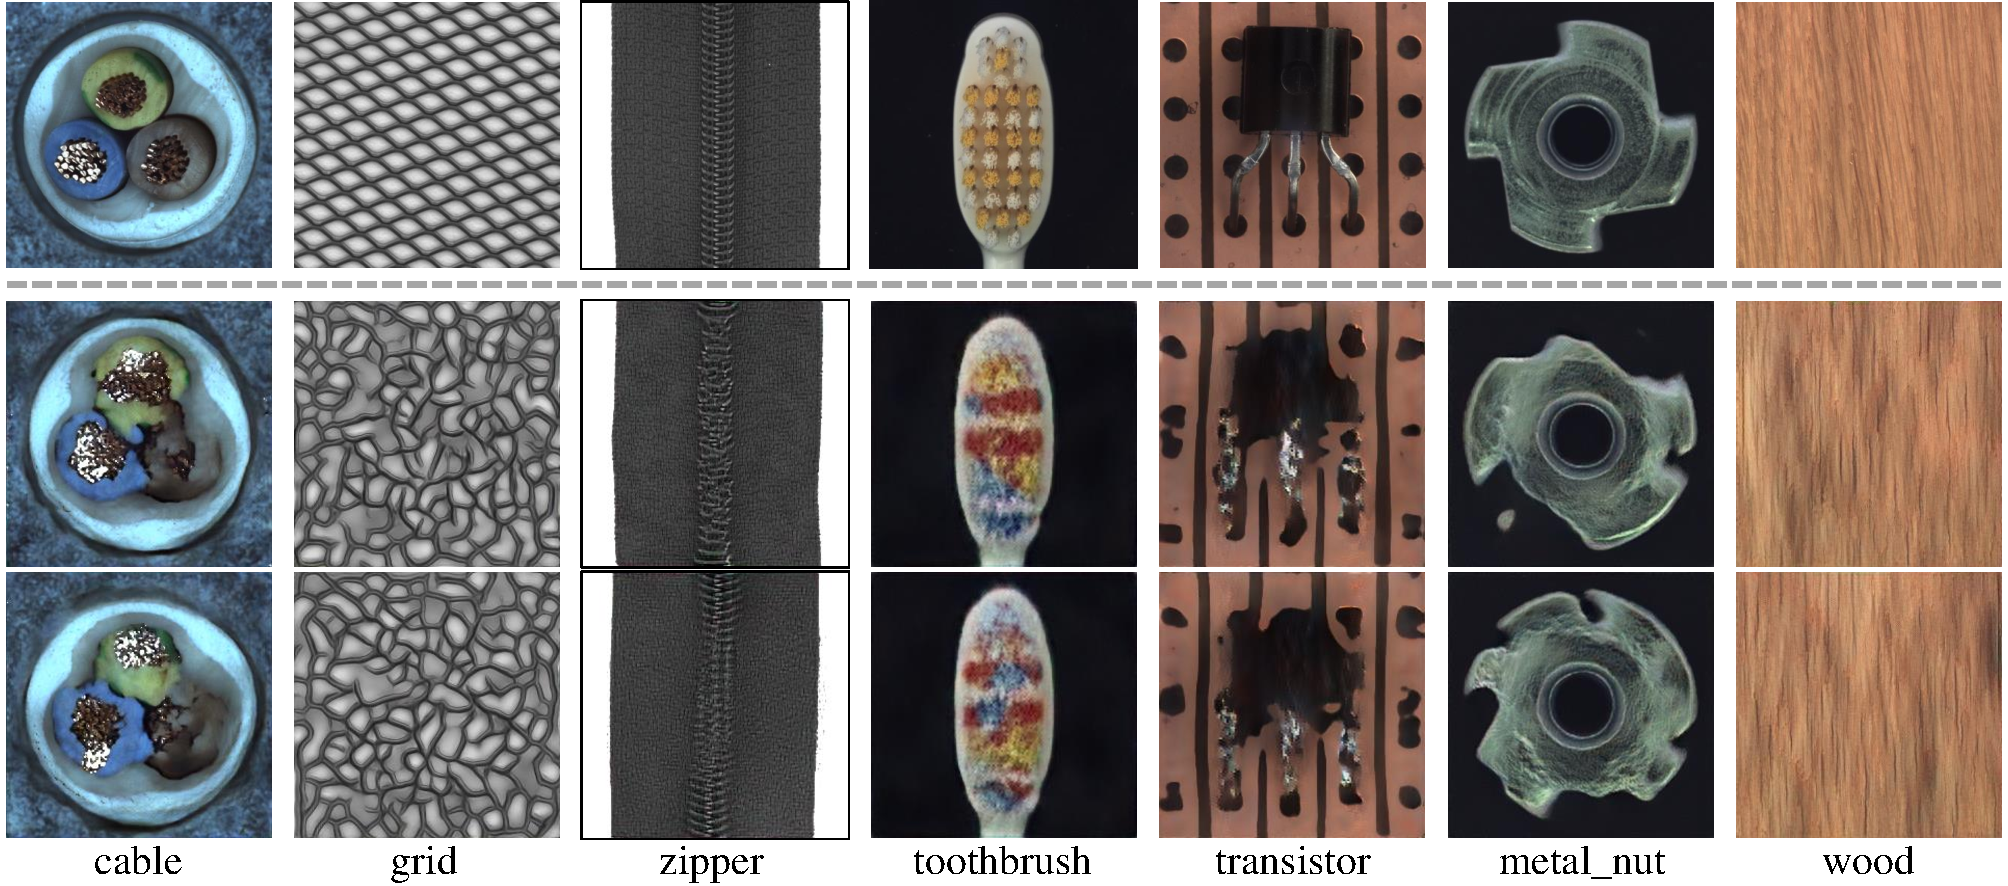
\includegraphics[width=0.7\linewidth]{images/mvtec_generation_results.pdf}
    \caption{Contrastive images generated by level-13 PatchDiff for MVTec AD~\cite{MVTecAD}. } 
    \label{fig: mvtec_generation}
\end{figure*}

\begin{table*}[!h]
    \centering
    % \footnotesize
    % \setlength{\belowcaptionskip}{0.2cm}
    % \setlength{\abovecaptionskip}{0.0cm}
    \renewcommand{\arraystretch}{1.2}
    \resizebox{\textwidth}{!}
    {
\begin{tabular}{cl|c|c|c|c|c|c|c|c}
\toprule
% \multicolumn{2}{c|}{Category} & \makecell[c]{IGD\\\tiny{\citealp{IGD}}} & \makecell[c]{PSVDD\\\tiny{\citealp{PSVDD}}} & \makecell[c]{FCDD\\\tiny{\citealp{FCDD}}} & \makecell[c]{CutPaste\\\tiny{\citealp{CutPaste}}} & \makecell[c]{NSA\\\tiny{\citealp{NSA}}} & \makecell[c]{DRAEM\\\tiny{\citealp{DRAEM}}} & \makecell[c]{DSR\\\tiny{\citealp{DSR}}} & \makecell[c]{GRAD\\\tiny{Ours}} \\ \midrule
\multicolumn{2}{c|}{Category}     & IGD & PSVDD & FCDD & CutPaste &NSA & DRAEM & DSR & GRAD \\ \midrule
\multirow{5}{*}{Texture} 
& carpet & (94.7, 82.8 ) & (92.9, 92.6) & (96.0, - ) & (93.1, 98.3) & (95.5, 95.6) & (95.5,97.0) & (-, \textbf{100.}) & (\textbf{96.5}, 98.2) \\
& grid & (97.7, 97.8 ) & (94.6, 100.) & (91.0, - ) & (\textbf{99.9}, 97.5) & (99.2, 99.9) & (99.7, 99.9) & (-, \textbf{100.}) & (97.2, \textbf{100.}) \\
& leather & (99.5, 95.8) & (90.9, 98.6) & (98.0, - ) & (\textbf{100.}, 99.5) & (99.5, 99.9) & (98.6, \textbf{100.}) & (-, \textbf{100.}) & (98.8, \textbf{100.}) \\
& tile & (78.0, 99.1) & (97.8, 91.4) & (91.0, - ) & (93.4, 90.5) & (\textbf{99.3}, \textbf{100.}) & (99.2, 99.6) & (-, \textbf{100.}) & (95.4, \textbf{100.}) \\
& wood & (89.1, 94.6) & (96.5, 90.8) & (88.0, - ) & (\textbf{98.6}, 95.5) & (90.7, 97.5) & (96.4, \textbf{99.1}) & (-, 96.3) & (87.2, 98.3) \\
\midrule
\multirow{10}{*}{Object} 
& bottle & (92.2, \textbf{100.}) & (98.6, 98.1) & (97.0, - ) & (98.3, 97.6) & (98.3, 97.7) & (\textbf{99.1}, 99.2) & (-, \textbf{100.}) & (96.5, \textbf{100.}) \\
& cable & (84.7, 90.6) & (90.3, 96.8) & (90.0, - ) & (80.6, 90.0) & (96.0, 94.5) & (94.7, 91.8) & (-, 93.8) & (\textbf{98.4}, \textbf{99.3}) \\
& capsule & (\textbf{97.7}, 91.5) & (76.7, 95.8) & (93.0, - ) & (96.2, 97.4) & (97.6, 95.2) & (94.3, \textbf{98.5}) & (-, 98.1) & (97.1, 96.4) \\
& hazelnut & (98.0, 99.7) & (92.0, 97.5) & (95.0, - ) & (97.3, 97.3) & (97.6, 94.7) & (\textbf{99.7}, \textbf{100.}) & (-, 95.6) & (96.6, 98.1) \\
& metal nut & (92.6, 91.3) & (94.0, 98.0) & (94.0, - ) & (99.3, 93.1) & (98.4, 98.7) & (\textbf{99.5}, 98.7) & (-, 98.5) & (93.7, \textbf{100.}) \\
& pill & (97.3, 87.3) & (86.1, 95.1) & (81.0, - ) & (92.4, 95.7) & (\textbf{98.5}, \textbf{99.2}) & (97.6, 98.9) & (-, 97.5) & (98.1, 95.7) \\
& screw & (97.0, 82.5) & (81.3, 95.7) & (86.0, - ) & (86.3, \textbf{96.7}) & (96.5, 90.2) & (97.6, 93.9) & (-, 96.2) & (\textbf{99.2}, 96.0) \\
& toothbrush & (97.7, 99.7) & (\textbf{100.}, 98.1) & (94.0, - ) & (98.3, 98.1) & (94.9, \textbf{100.}) & (98.1, \textbf{100.}) & (-, 99.7) & (98.0, 99.7) \\
& transistor & (84.4, 90.6) & (91.5, 97.0) & (88.0, - ) & (95.5, 93.0) & (88.0, 95.1) & (90.9, 93.1) & (-, 97.8) & (\textbf{97.8}, \textbf{100.}) \\
& zipper & (96.7, 97.0) & (97.9, 95.1) & (92.0, - ) & (\textbf{99.4}, 99.3) & (94.2, 99.8) & (98.9, \textbf{100.}) & (-, \textbf{100.}) & (98.3, 99.7) \\
\midrule
\multicolumn{2}{c|}{Average} & (93.1, 93.4) & (92.5, 93.2 ) & (92.1, 95.7) & (95.2, 96.0) & (96.3, 97.2) & (\textbf{97.3}, 98.0) & (-, 98.2) & (96.8, \textbf{98.7}) \\
\bottomrule
\end{tabular}}
\caption{Anomaly detection performance on MVTec AD dataset~\cite{MVTecAD}. Both pixel-level (left) and image-level (right) AUROC results are shown in each column. The best results are in bold.}
\label{tab: mvtec_main_detail}
\end{table*}

\subsection{Anomaly Detection and Localization}
In the main body, we exclusively present the averaged performance comparison on MVTec AD. In this section, we extend our analysis to provide a detailed result of the anomaly detection and localization performance across each individual sub-dataset within MVTec AD, and display anomaly maps on MVTec AD in Fig.~\ref{fig: main_mvtec_ad_results}. As shown in Table~\ref{tab: mvtec_main_detail}, we compare GRAD to IGD~\cite{IGD}, PSVDD~\cite{PSVDD}, FCDD~\cite{FCDD}, CutPaste~\cite{CutPaste}, NSA~\cite{NSA}, DRAEM~\cite{DRAEM}, and DSR~\cite{DSR}, all of which are independent of pretrained feature extractors. It is easy to find GRAD achieves a strong detection and localization of anomalies.  

\begin{figure*}[!h]
    \centering
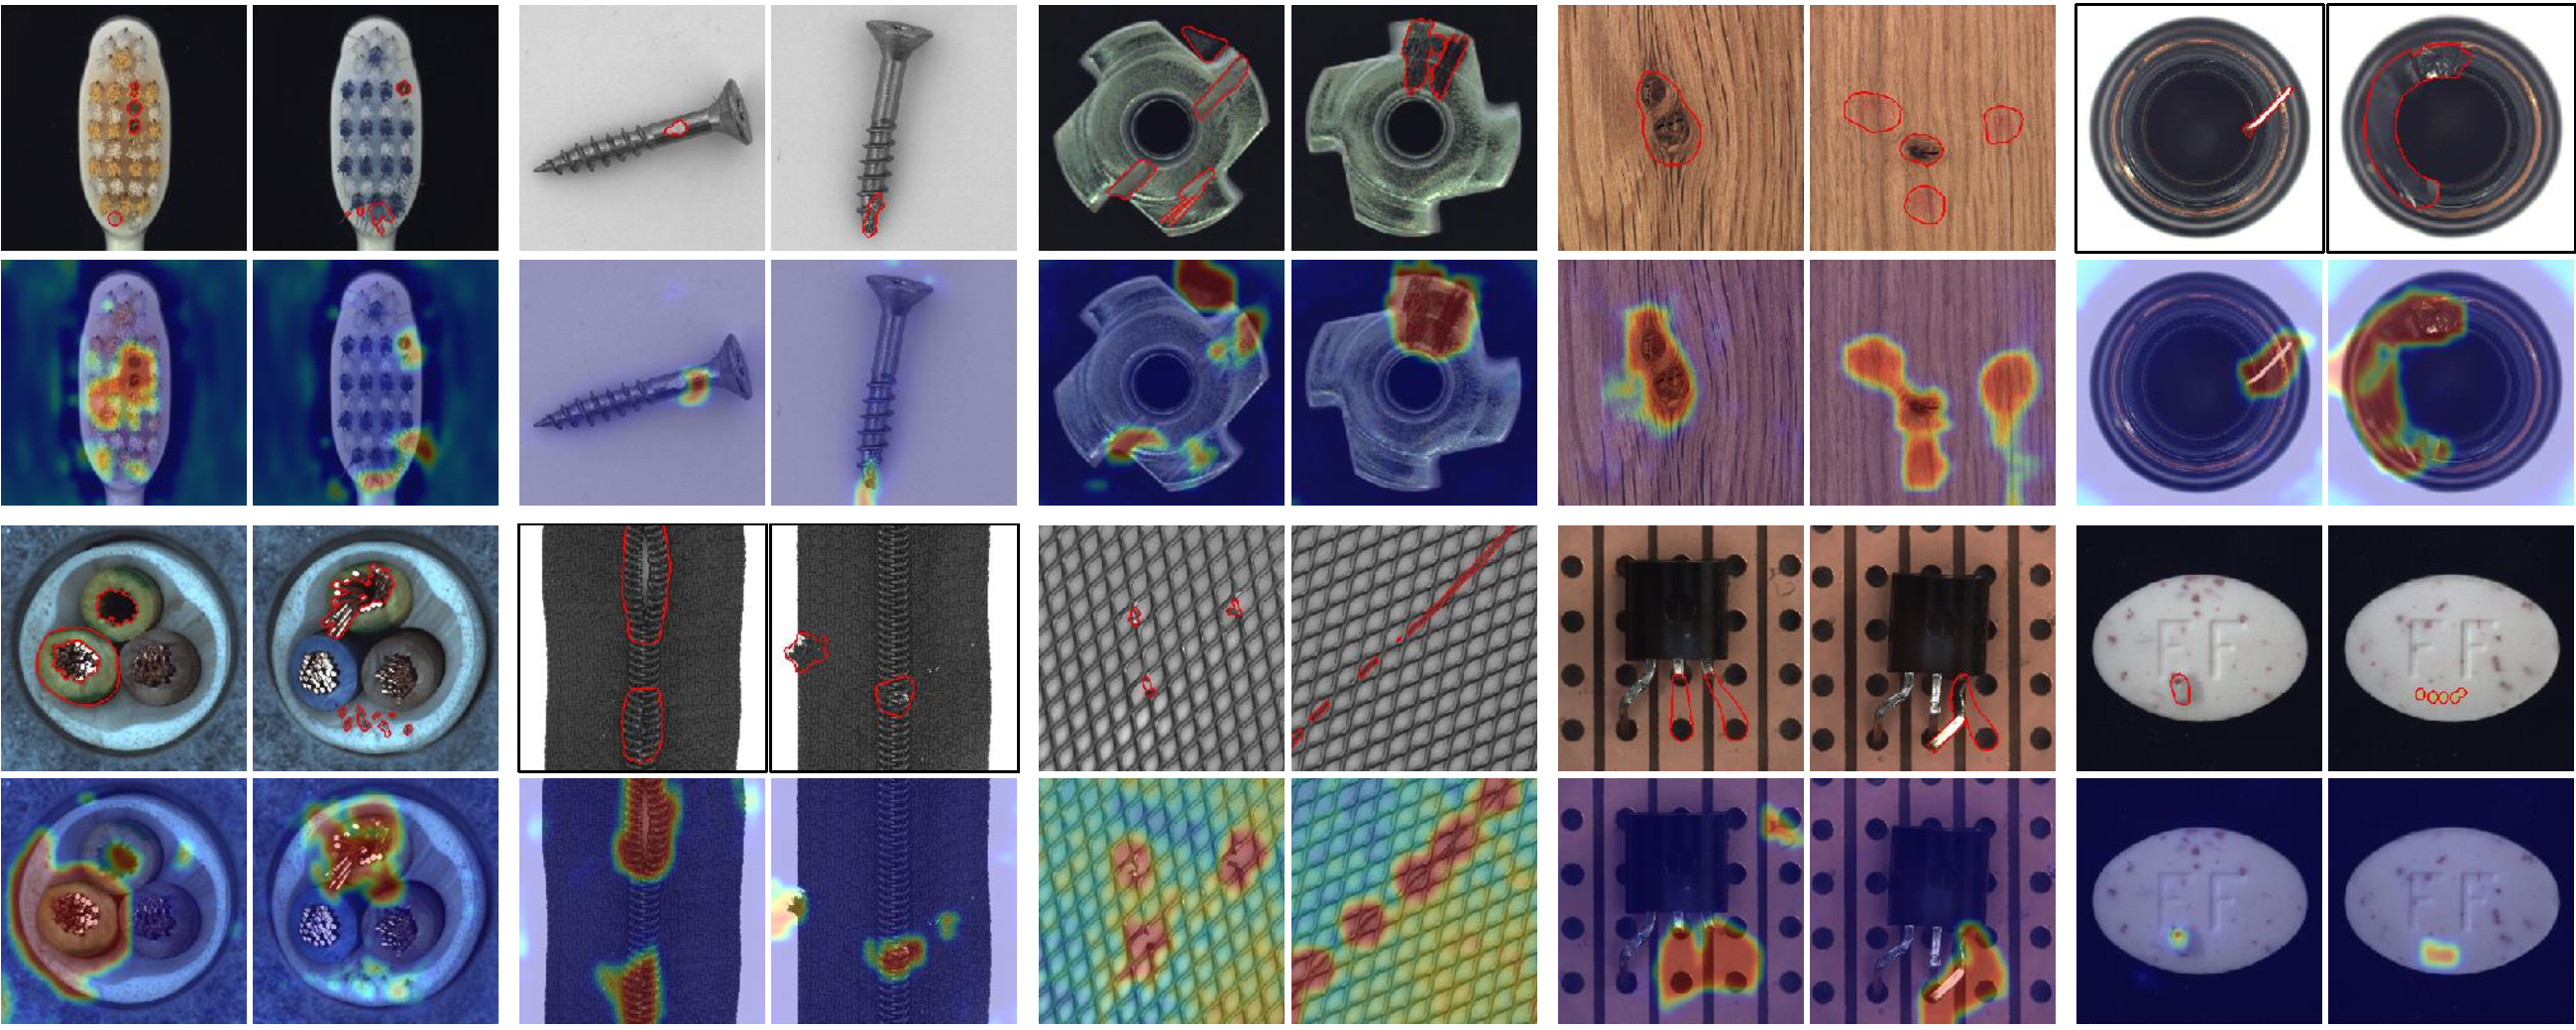
\includegraphics[width=0.9\linewidth]{images/mvtec_results.pdf}
    \caption{Defect localization results of GRAD on MVTec AD~\cite{MVTecAD}. } 
    \label{fig: main_mvtec_ad_results}
    % \vspace{-0.2cm}
\end{figure*}


% In addition, as shown in Table~\ref{tab:ablation_GRad_level}, we conduct an ablations study on selecting levels of patch-level detectors. It is easy to find that when integrating all three different levels of detectors, GRAD can achieve a strong performance for the detection of structural as well as logical anomalies.

% \begin{table}[!htbp]
% \centering
% \footnotesize
% \resizebox{0.3\textwidth}{!}{
% \begin{tabular}{ccc|c}
% \toprule
% \multicolumn{3}{c|}{Level Settings}& Image-level \\
% 136 & 68 & 34  & AUROC\\
% \midrule
% \checkmark &   \ding{55} & \ding{55}   &  85.2   \\
% \ding{55}& \checkmark & \ding{55} & 85.4 \\
% \ding{55}&\ding{55} & \checkmark & 75.1\\
% \checkmark & \checkmark & \ding{55}   &  86.8     \\ %
% \checkmark &   \ding{55} & \checkmark   &  86.4   \\
% \ding{55} & \checkmark & \checkmark  & 86.2 \\
% \checkmark & \checkmark & \checkmark &  \textbf{87.5}  \\
% \bottomrule
% \end{tabular}}
% \caption{Ablation study on detector levels. Detection AUROC results on MVTec LOCO dataset. The best results are in bold.}
% \label{tab:ablation_GRad_level}
% \end{table}



% \bibliography{aaai24}
% \bibliographystyle{aaai24}

% \end{document}



\end{document}
